\documentclass[11pt,letterpaper]{article}

\usepackage{pslatex}
%\usepackage{latexsym}
\usepackage[english]{babel}
\usepackage[utf8]{inputenc}
\usepackage{amsmath}
\usepackage{bm}
\usepackage{graphicx}
\usepackage{tikz}
\usepackage{xcolor}
\usepackage{url}
%\usepackage[colorinlistoftodos]{todonotes}
\usepackage{rotating}
\usepackage{natbib}
\usepackage{amssymb}

\usepackage{tikz-dependency}
\usepackage{longtable}


\newcommand{\R}[0]{\mathbb{R}}
\newcommand{\E}[0]{\mathbb{E}}
\newcommand{\Ff}[0]{\mathcal{F}}

\usepackage{multirow}

\newcommand{\soft}[1]{}
\newcommand{\nopreview}[1]{}
\newcommand\comment[1]{{\color{red}#1}}
\newcommand\mhahn[1]{{\color{red}(#1)}}

\usepackage{amsthm}

\newcommand{\thetad}[0]{{\theta_d}}
\newcommand{\thetal}[0]{{\theta_{LM}}}

\newcounter{theorem}
\newtheorem{proposition}[theorem]{Proposition}
\newtheorem{thm}[theorem]{Theorem}
\newtheorem{corollary}[theorem]{Corollary}
\newtheorem{question}[theorem]{Question}
\newtheorem{example}[theorem]{Example}


\frenchspacing
%\def\baselinestretch{0.975}

%\emnlpfinalcopy
%\def\emnlppaperid{496}

\title{Crosslinguistic Word Orders Enable an Efficient Tradeoff between Memory and Surprisal}
\author{Michael Hahn, Judith Degen, Richard Futrell}
\date{2018}

\begin{document}

\maketitle


%
\begin{abstract}

Online memory limitations are well-established as a factor impacting sentence processing and have been argued to account for crosslinguistic word order regularities. Building off expectation-based models of language processing, we provide an information-theoretic formalization of these memory limitations. We introduce the idea of a memory-surprisal tradeoff: comprehenders can achieve lower average surprisal per word at the cost of storing more information about past context. We show that the shape of the tradeoff is determined in part by word order. In particular, languages will enable more efficient tradeoffs when they exhibit information locality: when predictive information about a word is concentrated in the word’s recent past. We show evidence from corpora of 52 real languages showing that languages allow for more efficient memory-surprisal tradeoffs than random baseline word order grammars. 

%Are languages optimized for processing with limited memory?
%Memory limitations are well-established as a factor impacting sentence processing, and have been argued to account for crosslinguistic word order regularities.
%Computational models of language processing implementing memory constraints take various forms and make different kinds of assumptions about the architecture underlying human language processing.
%We first  establish general information-theoretic lower bounds on memory that hold in any model of language processing, applying both to speakers and listeners. %assuming only that listeners perform incremental prediction.
%Applying these results to corpora from over 50 languages, we then provide evidence that word orders in human language are optimized for memory demands of speakers and listeners. % producing language and listeners predicting input.
\end{abstract}


%
%
%\begin{thm}\label{prop:suboptimal}
%	For each positive integer $t$, define
%$I_t := I[X_t, X_0 | X_{1\dots t-1}]$,
%i.e., the mutual information between words at distance $t$, controlling for redundancy with the intervening words.
%	Let $T$ be a positive integer, and consider a comprehender using at most $\sum_{t=1}^T t I_t$
%bits of memory on average.
%Then this comprehender will incur average surprisal at least
%	$H[X_t|X_{<t}] + \sum_{t > T} I_t$.
%\end{thm}
%


\section{Introduction}

A wide range of work has argued that natural language orders information in ways that reduce memory effort.
An early example is \cite{miller-finitary-1963}, who attributed the unaccebtability of multiple center embeddings in English to limitations of human working memory.
\cite{hawkins-efficiency-2003} provides cross-linguistic evidence that word orders are optimized for processing based on local contexts.
Further work has found computational, corpus-based evidence that memory limitations impact language structure and production.
In particular, languages have been shown to shorten the length of syntactic dependency lengths \citep{futrell-large-scale-2015}.
Dependency length can be linked to memory use in certain models of incremental syntactic parsing, and increases processing difficulty in theories of memory in sentence processing \citep{gibson-linguistic-1998}.
\cite{gildea-human-2015} further provide evidence from five languages that word orders optimize predictability from local contexts.
\cite{futrell-noisy-context-2017} provide evidence that language shows information locality, i.e., elements with higher mutual infomation are closer together, which is predicted by their model of Lossy-Context Surprisal.

%TODO mention prior work
%
%-  center embeddings dispreferred/impossible to process \cite{miller-finitary-1963}
%
%- explanation of greenberg universals
%
%- dependency length minimization
%
%- \cite{gibson-linguistic-1998}
%

%\paragraph{\cite{berwick-grammatical-1986}}
%They considered incremental parsing, or, more precisely, incremental recognition of grammaticality.



%also (CITE): operations in a specific incremental parsing model

All these models of memory in sentence processing, and derived measures of efficiency for memory allocation, require specific assumptions about the architecture of memory.
This leaves open the question whether such assumptions are necessary, or whether word orders across languages are optimized for memory independently of the implementation and architecture of human language processing.


We approach this question by first providing general information-theoretic lower bounds on memory load that will hold independently of the architecture of memory representations.
We will consider a general setting of a speaker producing sentences from a language, and a listener performing incremental prediction.
Our result immediatly entails a link between boundedness of memory and locality, which had been stipulated or derived from assumptions about memory architecture in previous models \citep{gibson-linguistic-1998, lewis-activation-based-2005, futrell-noisy-context-2017}.
Unlike many previous theories, our results apply to both speakers and listeners.
We will then use corpus data from over 50 languages to provide evidence that their word orders help lower memory cost.


\section{Memory-Surprisal Tradeoff}

With minimal assumptions, we will use information theory to derive a tradeoff between \emph{listener memory} and (listener) surprisal

In the second part of the paper, we examine whether word orders in natural language optimise this tradeoff.


\subsection{Memory and Locality in General Sequence Models}

We consider a \emph{speaker} who produces sentences and a \emph{listener} who, as the speaker's utterance unfolds, engages in incremental prediction.
Informally, we expect that both speaker and listener will be affected by memory demands:
From the speaker's perspective, producing well-formed sentences will require information about what she has uttered so far.
From the listener's perspective, predicting the next word well requires maintaining information about the past.
For the listener, the quality of prediction is measured by the average \emph{surprisal} experienced.
For a fixed language, we can ask how much information about the past (1) the speaker has to maintain to produce well-formed utterances, and (2) the listener has to maintain to incur a minimal amount of surprisal.
Utilizing the tools of information theory, we quantify memory in \emph{bits}, obtaining bounds that hold across different models of memory architecture and ways of quantifying memory load.




We now make this more formal:
We think of the language as a stochastic process $(X_t)_{t \in \mathbb{Z}}$, that is, a probability distribution over sequences of words $\dots x_{-2} x_{-1} x_0 x_{1} x_{2} \dots$.
As the elements are indexed by the full set of integers, we think of the process as extending infinitely into both the past and the future; that is, we model a setting where the speaker has been speaking and will continue to speak for an infinite amount of time.
This assumption is for mathematical convenience and does not affect the substance of our results: As we restrict our attention to the processing of individual sentences, which have finite length, we will actually not make use of long-range and infinite contexts.
Second, we make the assumption that this process is \emph{stationary}.
Formally, this means that the conditional distribution $P(X_t|X_{<t})$ does not depend on $t$, it only depends on the actual sequence $X_{<t}$.
Informally, this says that the process has no `internal clock', and that the statistical rules of the language do not change at the timescale we are interested in.
In reality, the statistical rules of language do change: They change as language changes over generations, and they also change between different situations -- e.g., depending on the interlocutor at a given point in time.
Given that we are interested in memory needs in the processing of \emph{individual sentences}, at a timescale of seconds or minutes, stationarity seems to be a reasonable assumption to make.


The speaker maintains a memory state $S_t$, which evolves over the timesteps $t$.
We will not make any assumptions about the content of $S_t$ and how the speaker computes it.
The only assumption is that the speaker's past and future utterances are independent when conditioning on the memory state:
\begin{equation}\label{eq:markov-speaker}
X_{>t} \bot X_{\leq t} | S_t
\end{equation}
This means that the memory state $S_t$ functions as a `bottleneck', encoding all information about the past that influence the speaker's choices in the future.


We now analyze memory from the perspective of the listener, who needs to maintain information about the past to predict the future.
The listener maintains a memory state $L_t$; there are no assumptions about the memory architecture and the nature of its computations.
%We assume that the listener has no access to the speaker's state beyond what the speaker has already uttered.
We only make two basic assumptions about the flow of information:


We assume that $L_t$ contains no information about the process beyond what is contained in $X_{t-1}$ and $L_{t-1}$:
	\begin{equation}\label{eq:listener-markov}
p((X_{t})_t| L_0, L_1, X_1)   = p((X_{t})_t| L_0, X_1)
	\end{equation}

%
%First, we assume that the listener's internal state cannot depend on the future beyond its dependency on the past.
%Formally: 
%\begin{equation}\label{eq:listener-markov-1}
%L_t \bot X_{>t} | X_{\leq t}
%\end{equation}
%This means that the listener has no access to the speaker's state beyond what the speaker has already uttered.
%
%Second, we assume that $L_t$ contains no information about the past beyond what is contained in $X_{t-1}$ and $L_{t-1}$:
%\begin{equation}\label{eq:listener-markov-2}
%L_t \bot X_{<t} | X_{t-1}, L_{t-1}
%\end{equation}
%This means that any information about the past in $L_t$ has to be contained in $L_{t-1}$ -- formalizing the idea that a listener can only remember aspects of the past by keeping them in memory, and that memories of the past cannot `spontaneously' form later in the future.

The listener can trade off memory and future surprisal:
A listener who chooses to store less memory will exerience higher surprisal in the future.
A listener can achieve minimal surprisal -- that is, the lowest average surprisal that any model could achieve by predicting the future from the past -- if and only if $L_t$ contains all predictive information about the future that is contained in the past.

We will describe this tradeoff, and show that listener memory is linked to locality in a way similar to speaker memory.
Consider a listener who uses $J$ bits of memory on average.
What can we say about the listener's surprisal?
We return to the information and memory curves in Figure~\ref{fig:basic}.
In the graph of $t \cdot I_t$, we look for the first $T$ such that the area under the curve to the left of $T$ has size $\geq J$.
This is illustrated in Figure~\ref{fig:listener-tradeoff-decay} (right).
Then let $\epsilon$ be the area under the curve of $I_t$ to the right of $T$ (Figure~\ref{fig:listener-tradeoff-decay}, left).
We can prove that such a listener must incur surprisal at least $\epsilon$ greater than a listener with perfect memory.
As before, we write $$I_t := I[X_t, X_0 | X_{1\dots t-1}]$$
Then


\begin{proposition}\label{prop:suboptimal}
	Let $T$ be a positive integer, and consider a listener using at most
$$\sum_{t=1}^T t I_t$$
bits of memory on average.
Then this listener will incur surprisal at least
	$$H[X_t|X_{<t}] + \sum_{t > T} I_t$$
	on average.
\end{proposition}


The proposition gives us a lower bound on the listener's memory-surprisal curve: Taking all pairs of memory $\sum_{t=1}^T t I_t$ and surprisal $H[X_t|X_{<t}] + \sum_{t > T} I_t$, we obtain a curve in memry-surprisal plane, which is a lower bound on the memory demands of any listener at a given surprisal level.
We visualize this for the two processes from Figure~\ref{fig:basic} in Figure~\ref{fig:listener-tradeoff}.

\begin{figure}
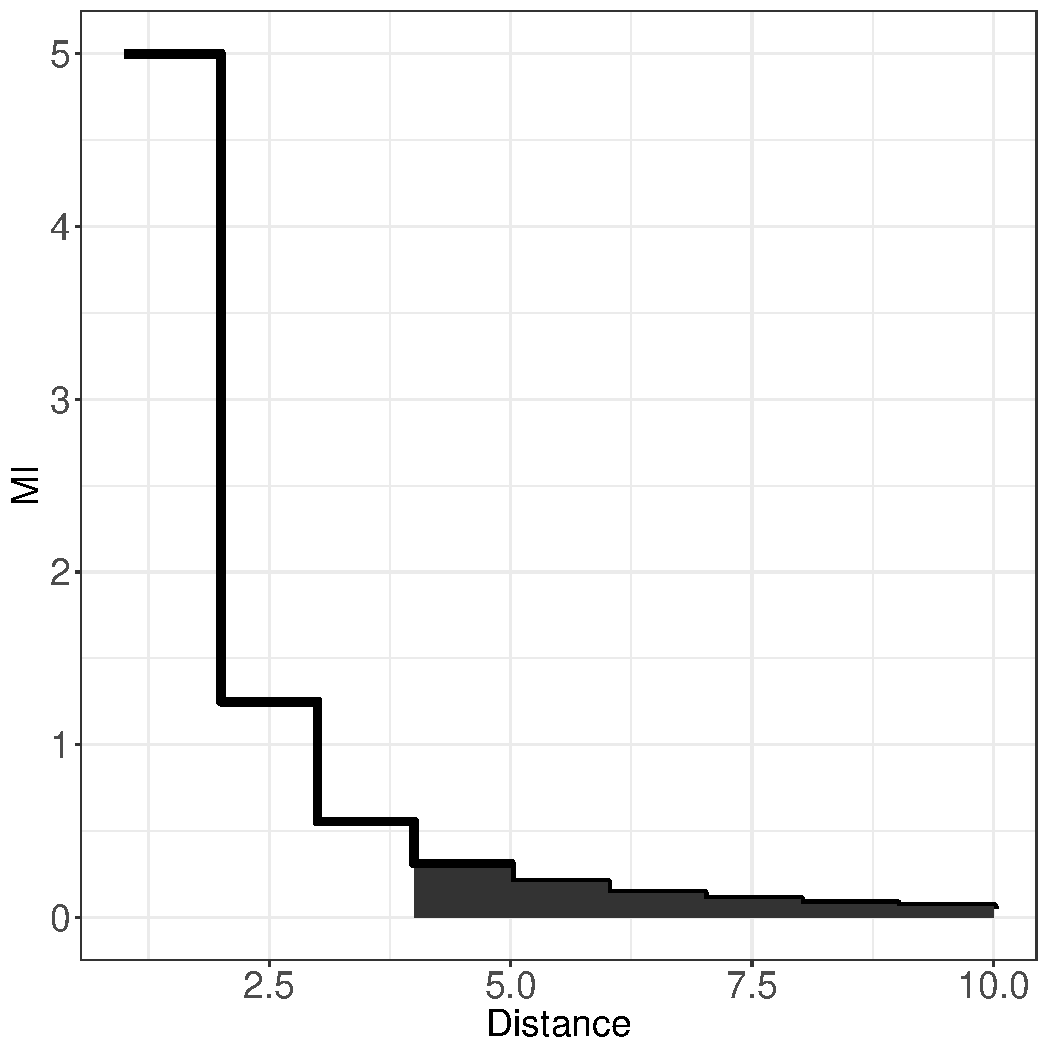
\includegraphics[width=0.45\textwidth]{toy/add-surp.pdf}
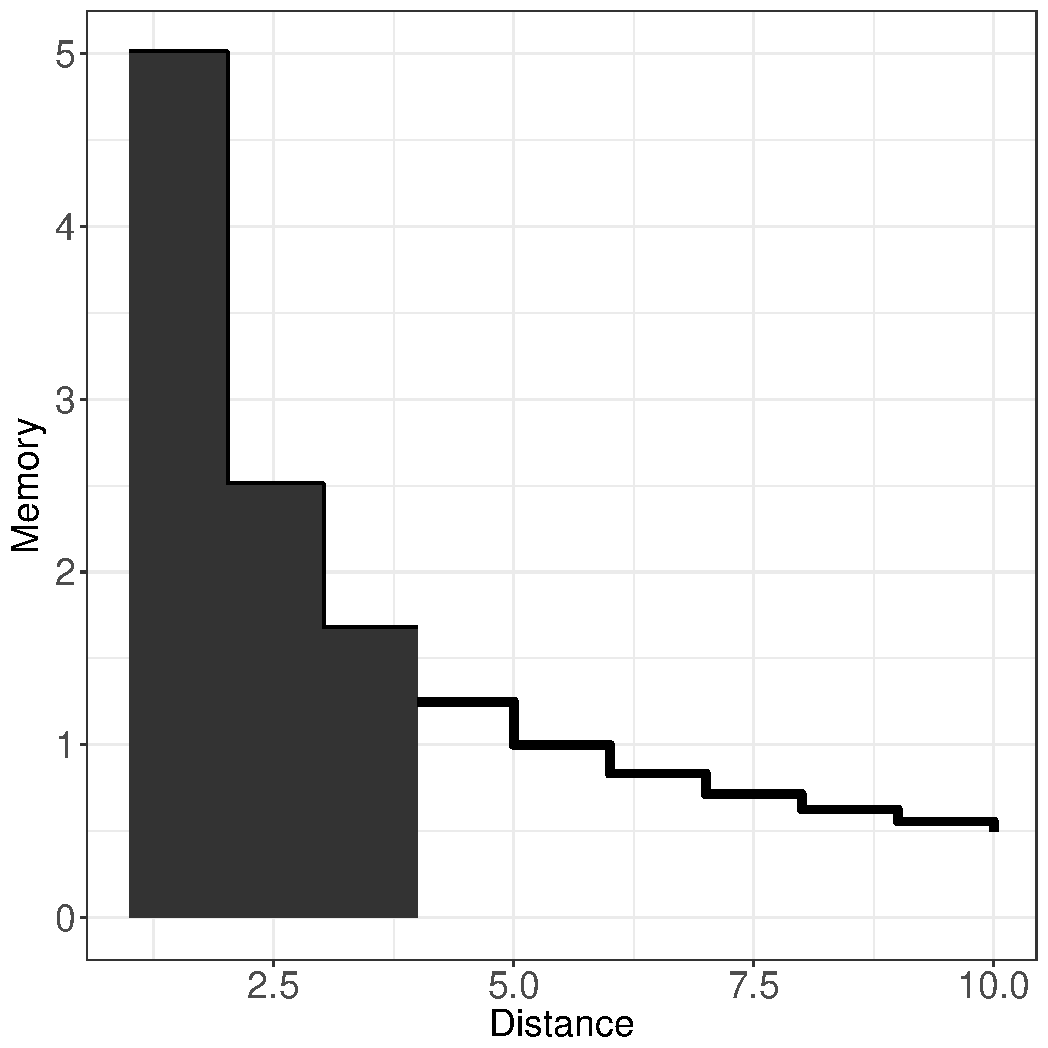
\includegraphics[width=0.45\textwidth]{toy/lower-mem.pdf}
	\caption{Illustration for Proposition~\ref{prop:suboptimal}. Listeners can trade off memory and surprisal: A listener only investing memory of the amount given by the black area on the right will incur at least the black area on the left in additional surprisal. In the given example, $T=4$. By varying $T$, the two areas describe the listener's memory-surprisal tradeoff curve.}\label{fig:listener-tradeoff-decay}
\end{figure}




\begin{figure}
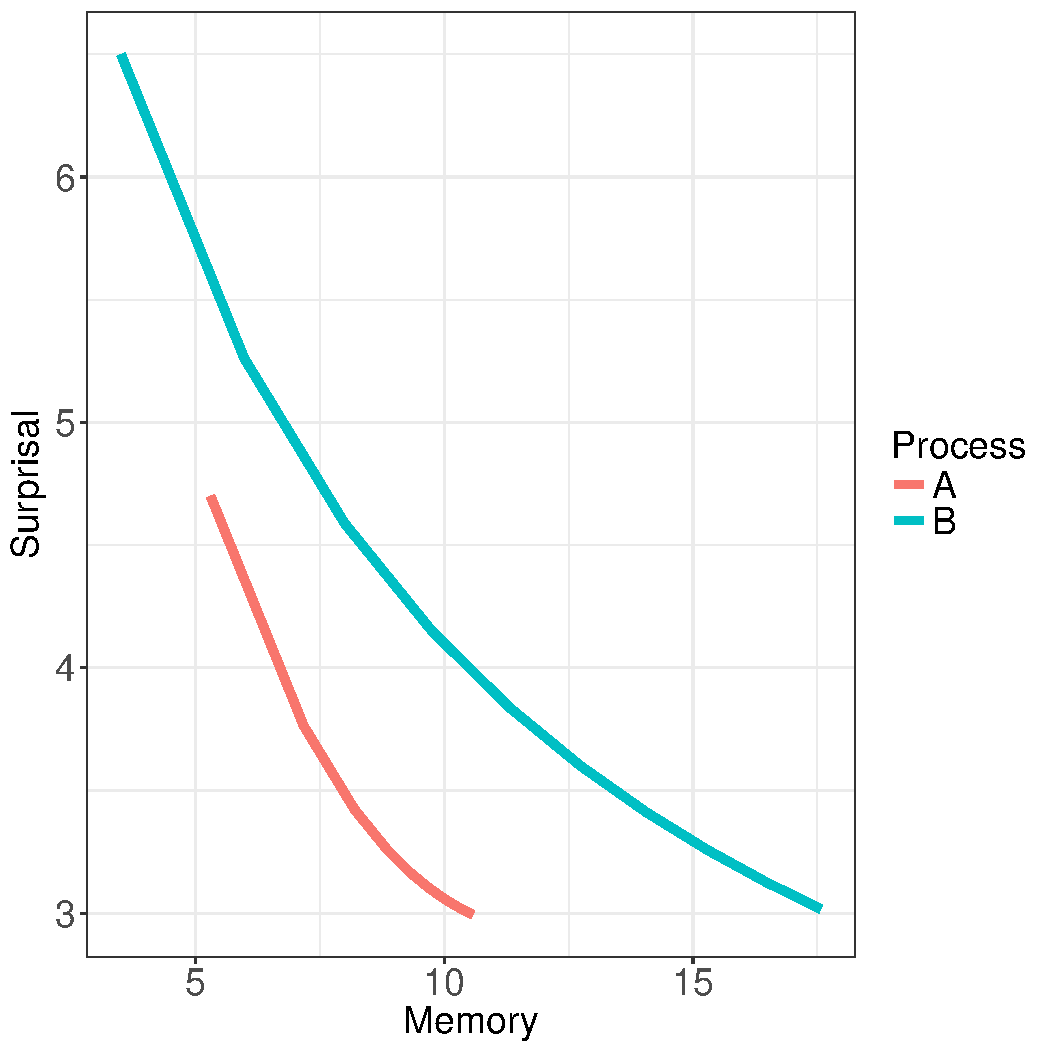
\includegraphics[width=0.45\textwidth]{toy/listener-tradeoff.pdf}
	\caption{Listener's memory-surprisal tradeoff for the two processes in Figure~\ref{fig:basic}. Recall that the red process had a faster decay of conditional mutual information. Correspondingly, this figure shows that a listener can achieve lower surprisal at the same level of memory load.}\label{fig:listener-tradeoff}
\end{figure}


In Figure~\ref{fig:toy-listener-tradeoff}, we show the resulting curve for the two versions of the artificial language from \cite{fedzechkina-human-2017}.
In this language, speaker memory coincides with the memory demand of a listener who performs optimally in incremental prediction.
The curve shows that, at any desired level of surprisal, Order A requires at most as much memory as Order B.
For reaching optimal surprisal, Order A requires strictly less memory.
Thus, in this case, the listener's surprisal-memory tradeoff is optimized by the orders predicted by Dependency Length Minimization.

\begin{figure}
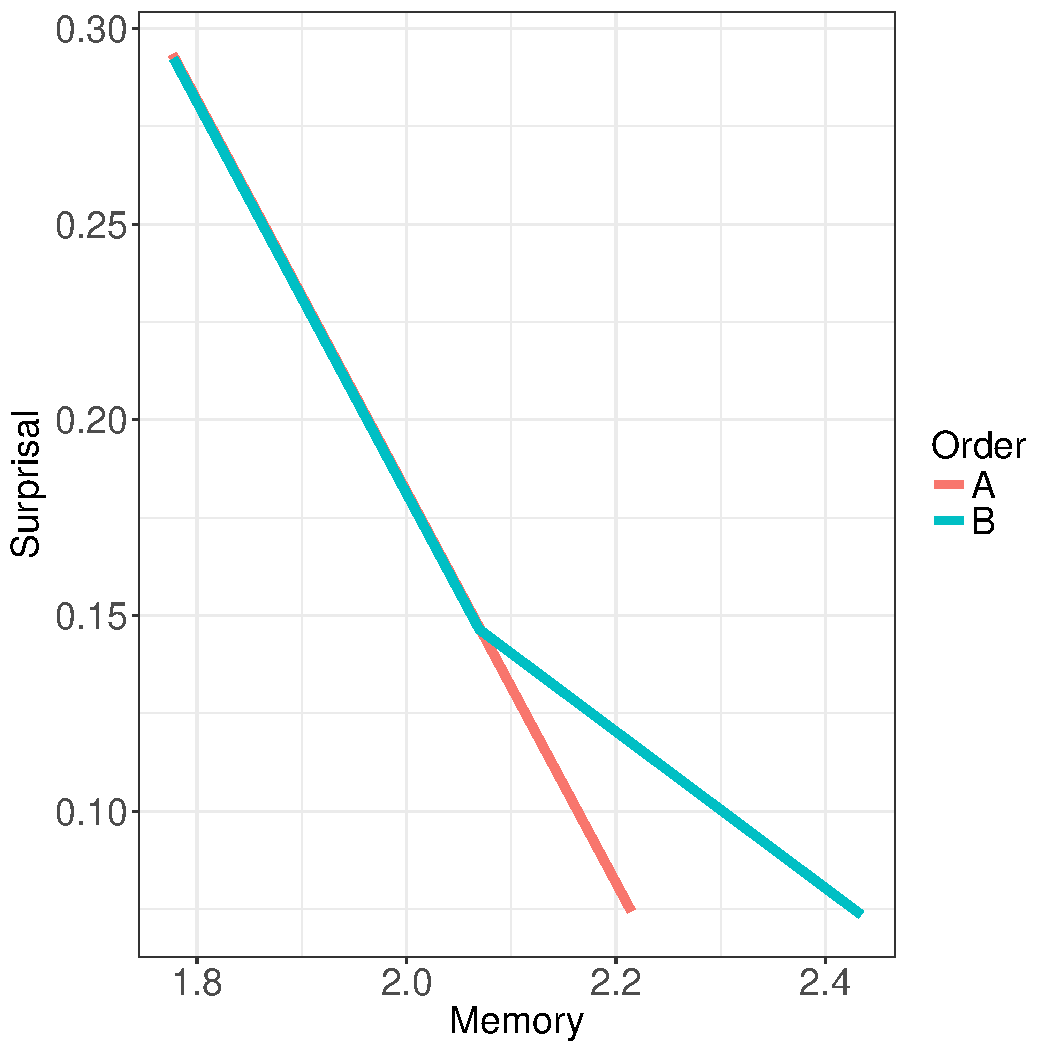
\includegraphics[width=0.45\textwidth]{toy/toy-mem-surp.pdf}
	\caption{Tradeoff between listener memory and surprisal, for the two versions of the artificial language from \cite{fedzechkina-human-2017}. Language A requires less memory at the same level of surprisal.}\label{fig:toy-listener-tradeoff}
\end{figure}





\begin{figure*}
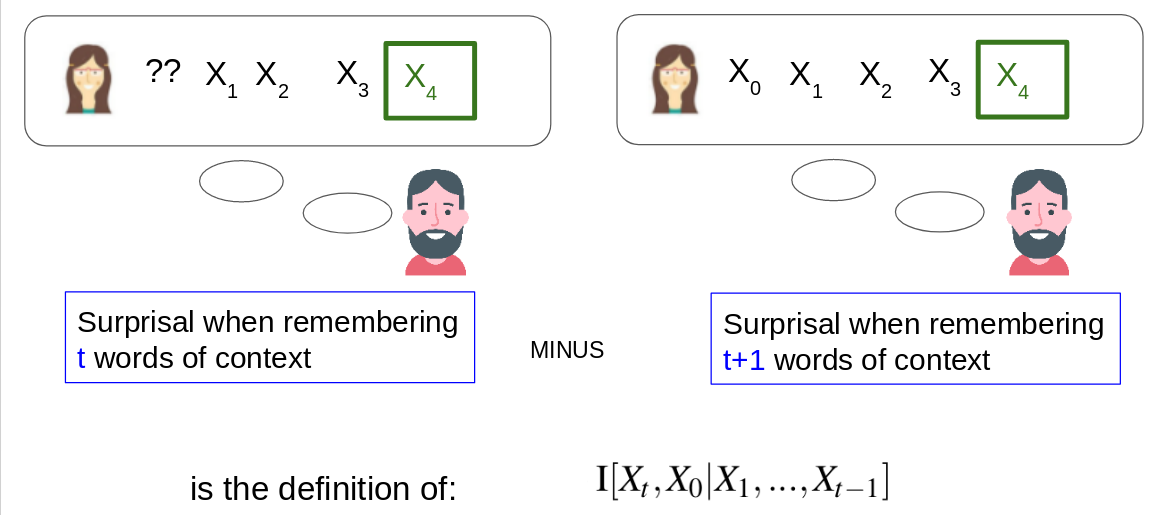
\includegraphics[width=0.9\textwidth]{figures/listener-it.png}
	\caption{(TODO adapt to format) Intuitive explanation of $I_t$}
\end{figure*}








We will use the concept of \emph{conditional mutual information}.
For two random variables $X, Y$, the mutual information $I[X,Y]$ is the reduction in entropy about $X$ by knowing $Y$:
\begin{equation}
	I[X,Y] := H[X] - H[X|Y]
\end{equation}
For three random variables $X, Y, Z$, the mutual information between $X$ and $Y$, conditional on $Z$, is this entropy reduction when $Z$ is already known:
\begin{equation}
I[X,Y|Z] := H[X|Z] - H[X|Z,Y]
\end{equation}
We will use the specific form where $X$ and $Y$ are observations $X_0$, $X_t$ of the process $(X_t)_{t \in \mathbb{Z}}$, and $Z$ is a block of intervening observations $X_1, \dots, X_{t-1}$:
\begin{equation}
	I[X_t, X_0 | X_1, \dots, X_{t-1}] := H[X_t| X_1, \dots, X_{t-1}] - H[X_t| X_0, X_1, \dots, X_{t-1}]
\end{equation}
This is equal to the reduction in uncertainty about the $t$-th observation when knowing the $0$-th observation, in addition to the block of intervening observations.
That is, we measure the amount of statistical dependency of observations that are $t$ steps apart, controlling for any information that is redundant with intervening observations.
This quantifies how much information needs to be carried across $t$ timesteps without any possibility for `guessing' it from intervening observations.



%that the model does not have an `absolute clock' built into it.
The quantity $M$ is equal to the mutual information between past and future observations, $I[(X_i)_{i>0}, (X_i)_{i \leq 0}]$, which is often referred to as the \emph{excess entropy} of the process (CITE).




Due to the factor $t$ inside each term of the sum, carrying the same amount of information over longer distances requires more memory -- that is, modeling long statistical dependencies is more costly in terms of memory than modeling shorter ones.
This formalizes a general, assumption-free, link between memory and locality in language production.
In Section~\ref{sec:listener}, we will extend this analysis to listeners performing incremental prediction.
%incremental prediction.


The result in (\ref{eq:memory-bound}) is entirely information-theoretic and applies to \emph{any} physical encoding of the past, entirely independent of the implementation of the model. % and the mechanisms by which it computes predictions.
In particular, while the relation to psycholinguistic and psychological models of how memory works will be interesting to explore, our result applies to any such model.
Memory representations do not have to be rational or optimal for this bound to hold:
It provides a \emph{lower bound} on the amount of information that needs to be stored -- other memory representations will always need to store at least as much information.

We will write $I_t$ as an abbreviation for $\operatorname{I}[X_t, X_0 | X_1, ..., X_{t-1}]$.
The proposition implies that memory is decreased if $I_t$ decreases quickly as $t \rightarrow \infty$ -- that is, if the contributions of long-term dependencies in the process are small.
In particular, memory load can only be finite if $I_t$ decreases fast enough for the infinite sum to converge to a finite value.
%This confirms the intuition that finiteness of memory entails that the contribution of long-term 

We have treated the process $(X_t)_t$ as a discrete-time process whose time steps correspond to words, but this is immaterial to the analysis.
The analysis is not even restricted to discrete timesteps: We can replace the sum in~(\ref{eq:memory-bound}) with an integral to get a continuous-time version.



We illustrate Proposition~\ref{prop:lower-bound} in Figure~\ref{fig:basic}.
We consider two processes A and B, where $I_t := 5t^{-1.5}$ for $A$ and $I_t := 3.5 t^{-2.5}$ for $B$.
The curves of $I_t$, as a function of the distance $t$, are shown in Figure~\ref{fig:basic} (left).
In both cases, $I_t$ converges to zero as $t$ grows to infinity. 
However, $I_t$ decays more quickly for Process A (red).
This means that predictive information about an observation is concentrated more strongly in the recent past.
In Figure~\ref{fig:basic} (right), we show $t\cdot I_t$ as a function of $t$.
Note that the area under the curve is equal to (\ref{eq:memory-bound}).
This area is smaller for the red process, as $I_t$ decays more quickly there.  


\begin{figure*}
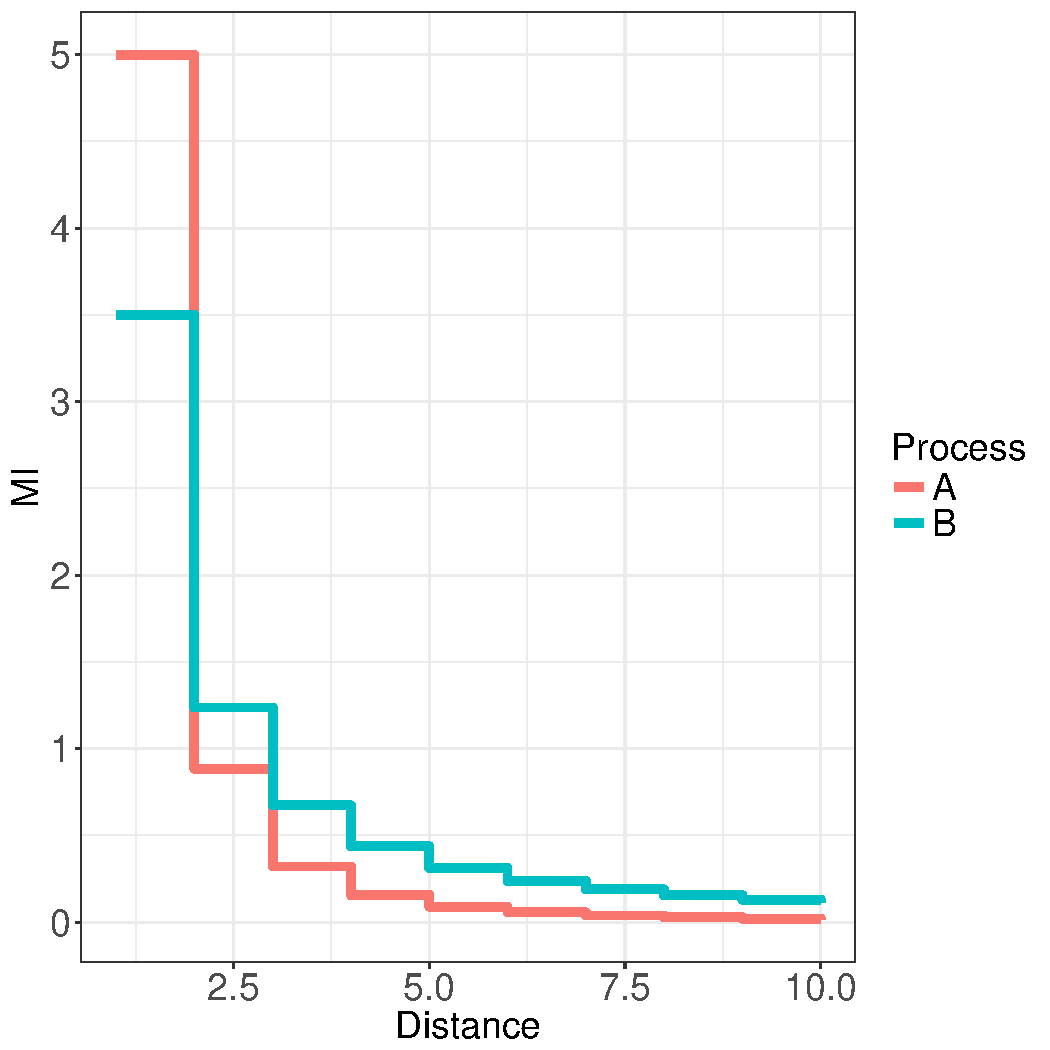
\includegraphics[width=0.45\textwidth]{toy/decay.pdf}
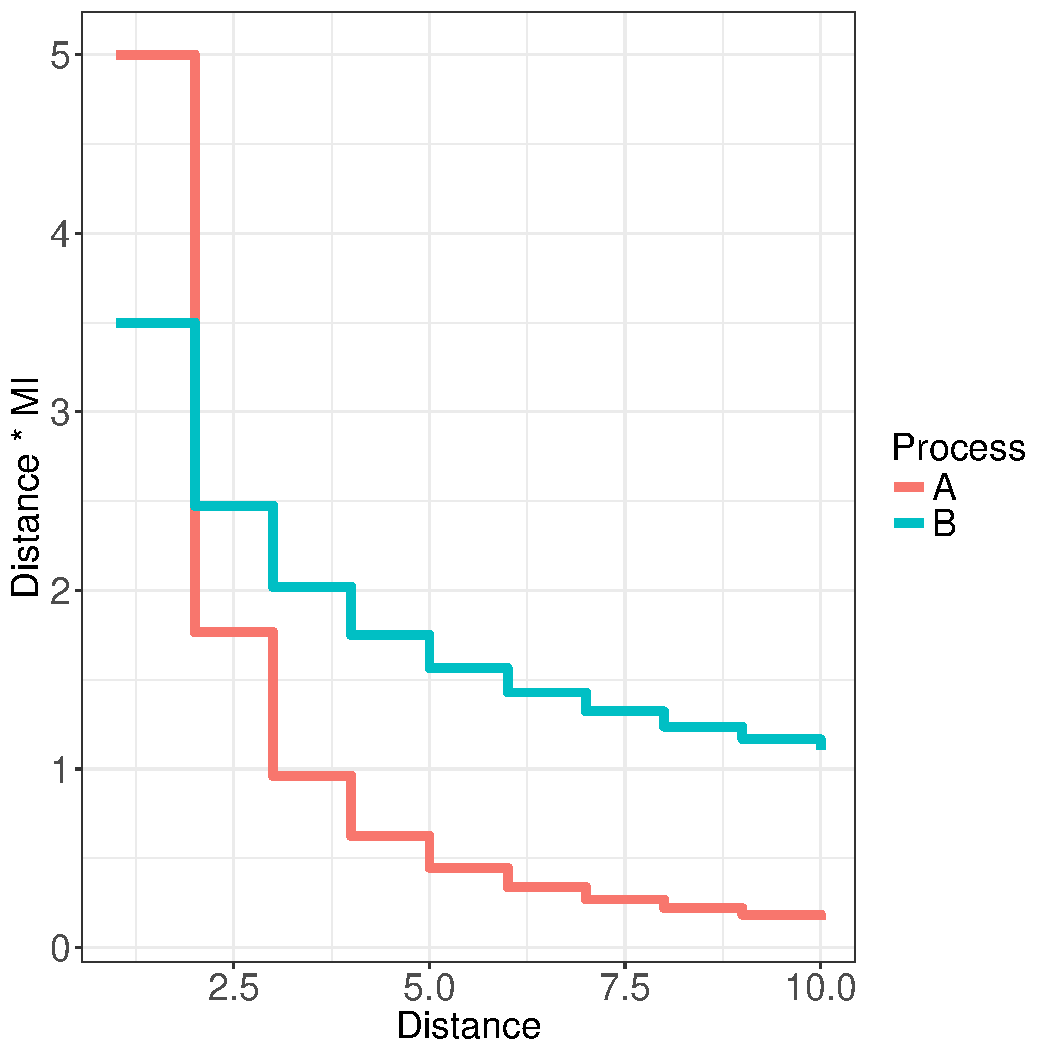
\includegraphics[width=0.45\textwidth]{toy/memory.pdf}
%
	\caption{Left: $I_t$ as a function of $t$, for two different processes. $I_t$ decays faster for the red process: Predictive information about the present observation is concentrated more strongly in the recent past. Left: $t \cdot I_t$ as a function of $t$ for the same processes. The area under the curves is given by (\ref{eq:memory-bound}). This area is smaller for the red process, as $I_t$ decays more quickly there.   }\label{fig:basic}
\end{figure*}


\subsection{Memory and Dependency Length}




We illustrate the linguistic predictions of Proposition \ref{prop:lower-bound} by reanalyzing the data from \cite{fedzechkina-human-2017}.
This is a miniature artificial language study that showed a bias for Dependency Length Minimization in production in artificial language learning.
Due to the controlled setting, it is possible to exactly compute the speaker's memory as given in~(\ref{eq:memory-bound}).


As ~(\ref{eq:memory-bound}) is invariant under reversal of the language, we only consider the head-final version of her artificial language.
The language has consistent head-final order, and uses case marking on objects.
The relevant production targets are transitive sentences where one of the two arguments is much longer than the other, due to the presence of a PP modifier, as shown in Table~\ref{tab:artificial}.
The language has variable order of subjects and objects; for the production targets, the B versions produce much longer dependencies than the A versions.
Dependency Length Minimization thus predicts that speakers are more likely to use the A versions.
\cite{fedzechkina-human-2017} confirmed this experimentally.


\begin{table}
	\textbf{A Orders: Short Dependencies}

		\begin{tabular}{ccc}
			Object & Subject & Verb \\
			\fbox{\begin{tabular}{llllll}
				\fbox{\begin{tabular}{llll} Adjective &Noun &Postposition\end{tabular}} & Noun-Case
					\end{tabular}} & \fbox{\begin{tabular}{l}Noun\end{tabular}} & \fbox{\begin{tabular}{l}Verb\end{tabular}}  \\
		\end{tabular}
\\
		\begin{tabular}{ccc}
			Subject & Object & Verb \\
			\fbox{\begin{tabular}{llllll}
				\fbox{\begin{tabular}{llll} Adjective &Noun &Postposition\end{tabular}} & Noun
					\end{tabular}} & \fbox{\begin{tabular}{l}Noun-Case\end{tabular}} & Verb \\
		\end{tabular}
\\
\\

	\textbf{B Orders: Long Dependencies}


		\begin{tabular}{ccc}
			Subject & Object & Verb \\
			 \fbox{\begin{tabular}{l}Noun\end{tabular}} &  \fbox{\begin{tabular}{llllll}
				\fbox{\begin{tabular}{llll} Adjective &Noun &Postposition\end{tabular}} & Noun-Case
		\end{tabular}}  &  \fbox{\begin{tabular}{l}Verb\end{tabular}}  \\
		\end{tabular}
\\
		\begin{tabular}{ccc}
			Object & Subject & Verb \\
			\fbox{\begin{tabular}{l}Noun-Case\end{tabular}} & \fbox{\begin{tabular}{llllll}
				\fbox{\begin{tabular}{llll} Adjective &Noun &Postposition\end{tabular}} & Noun
		\end{tabular}} & Verb \\
		\end{tabular}

			\caption{Production targets in the artificial mini language from \cite{fedzechkina-human-2017}. The language has head-final order, with free variation between SO and OS orders. When one of the arguments is much longer than the other, placing the longer one first (`A' orders) shortens syntactic dependencies, compared to `B' orders.}\label{tab:artificial}

\end{table}

In this section, we show that our bound on speaker memory makes the same prediction, without reference to syntactic structure or specific memory architectures. 

We constructed one language consisting of the A versions, and one language consisting of the B versions.
Following the experimental setup of \cite{fedzechkina-human-2017}, we assigned equal probability to the two possible configurations per language, and used a separate set of nouns (inanimate nouns) for the embedded noun in the long phrase.

We interpreted each of the two languages as a stationary processes, extending infinitely in both directions, by concatenating independent samples drawn from the language.
			We computed (\ref{eq:memory-bound}) from a chain of 1000 independently sampled sentences, for each of the two versions of the toy language.
			Figure~\ref{fig:toy-mis} (left) shows the curve of the conditional mutual information $I_t$ as a function of the distance $t$.
			The curves differ at $t=2$ and $t=5$: 
			About 0.073 nats of predictive information that are at distance $t=2$ in the A orders are moved to $t=5$ in the B orders.
%			In this sense, A orders have greater information locality than the B orders.
			%What is responsible for this difference?
			The source of the difference lies in predicting the presence and absence of a case marker on the second argument -- i.e., whether to anticipate a subject or object.
			In the A orders, considering the last two words is sufficient to make this decision.
			In the B orders, it is necessary to consider the word before the long second constituent, which is five words in the past.

			The total amounts of predictive information -- corresponding to the area under the curve -- are the same, indicating that both languages are equally predictable.
			However, we will see that the memory demands are different:
			Figure~\ref{fig:toy-mis} (right) shows $t\cdot I_t$ as a function of $t$.
			As $I_t$ decays faster in A orders, the total area under the curve now differs between A and B, and is larger in B.
			This area corresponds to the lower bound in (\ref{eq:memory-bound}), and is 2.21 nats in A orders, and 2.43 nats in B orders.
			While (\ref{eq:memory-bound}) is a general lower bound, it can be proven that this bound is actually tight in the case of this specific example.\footnote{This can be shown by computing the causal states and then showing that the crypticity is zero, both of which is tractable in the case of this small-scale artificial language.}
That is, a speaker who optimally allocates memory resources will spend 2.21 nats in A orders, and 2.43 nats in B orders.
It is important to stress that, even though we computed this value by considering the number of words impacting predictions at a given point in time, this bound holds independently of the actual implementation and architecture of memory and predictions.


\begin{figure*}
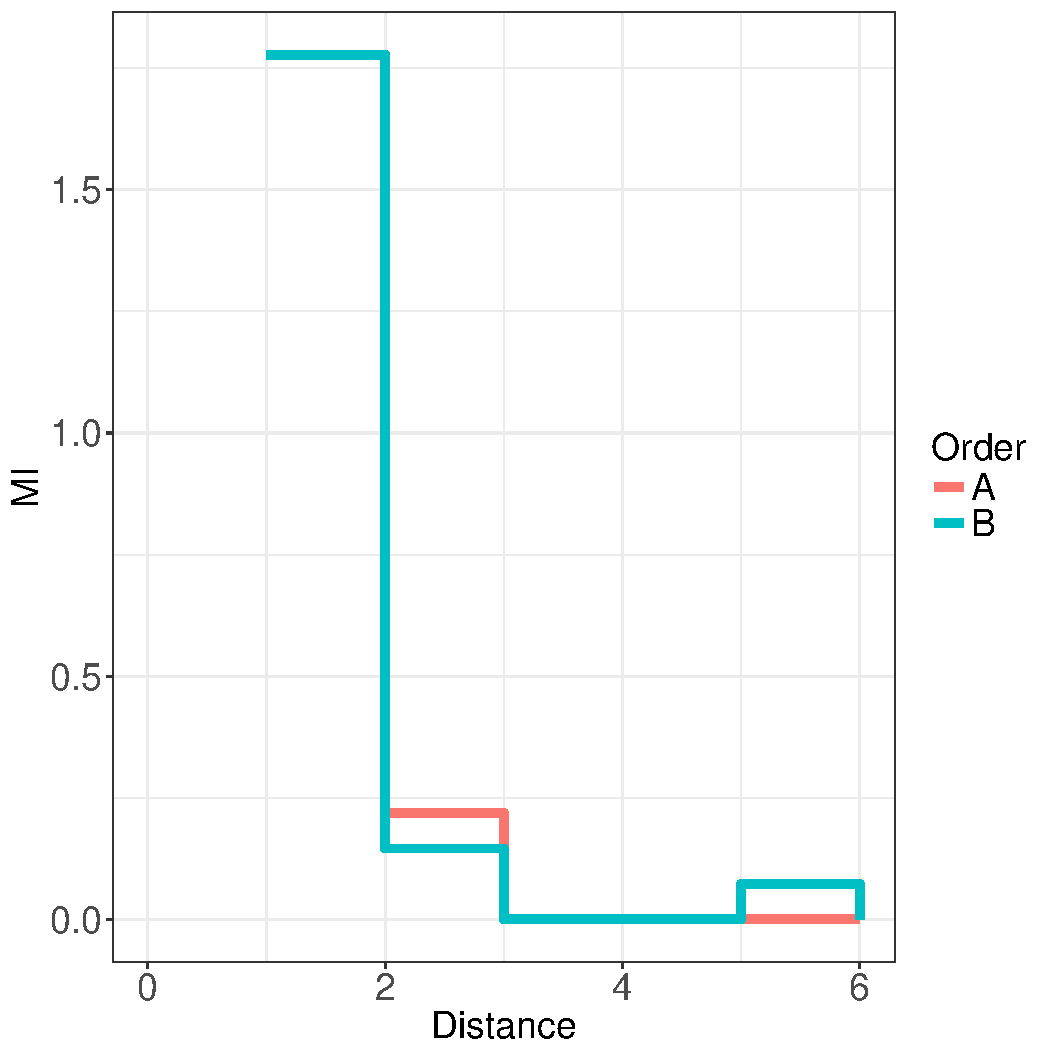
\includegraphics[width=0.45\textwidth]{toy/toy-mis.pdf}
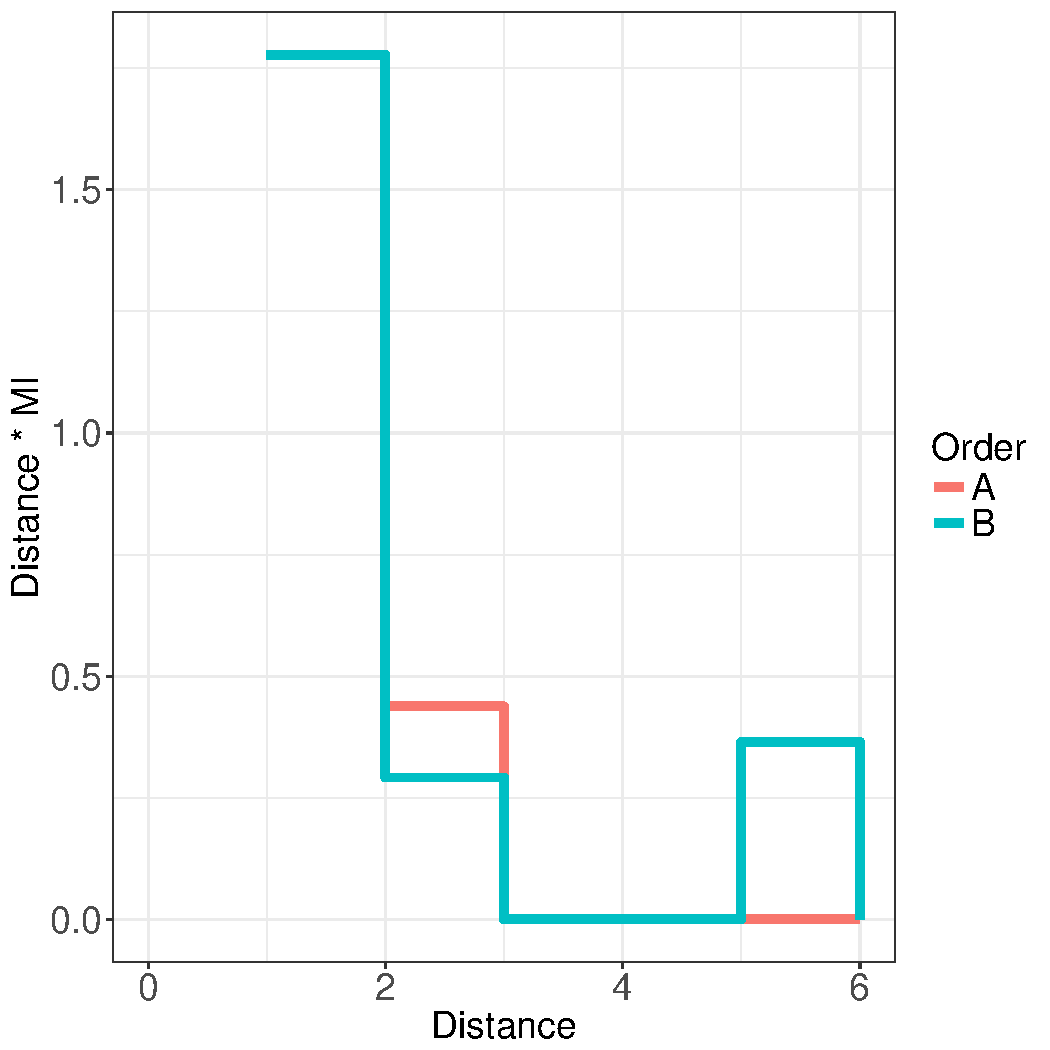
\includegraphics[width=0.45\textwidth]{toy/toy-t-mis.pdf}
%
	\caption{Left: Decay of Conditional Mutual Information, as a function of the distance $t$, for the two versions in the artificial language. The areas under the two curves are identical, corresponding to the fact that both orders are equally predictable. However, mutual Information decays faster in Order A.\ \ \ Right: $t I_t$, as a function of $t$. The area under the B curve is larger, corresponding to larger memory demand for this order.}\label{fig:toy-mis}
\end{figure*}
%Both languages have the same overall entropy rate, but they differ in the distribution of predictive information.
%
%plot of $I_t$
%
%The areas under the curves are identical.
%
%good version
%
%%CONTEXT LENGTH 0   2.06856758681  9997.93143241   0.0
%%CONTEXT LENGTH 1   0.29195106479  1.77661652202   1.77661652202
%%CONTEXT LENGTH 2   0.0729865489103  0.21896451588   2.21454555377
%%CONTEXT LENGTH 3   0.0729865489103  0.0   2.21454555377
%%CONTEXT LENGTH 4   0.0729865489103  0.0   2.21454555377
%%CONTEXT LENGTH 5   0.0729865489103  0.0   2.21454555377
%%CONTEXT LENGTH 6   0.0729865489103  0.0   2.21454555377
%
%bad version
%
%%CONTEXT LENGTH 0   2.06937301571  9997.93062698   0.0
%%CONTEXT LENGTH 1   0.291673373027  1.77769964269   1.77769964269
%%CONTEXT LENGTH 2   0.145830550934  0.145842822093   2.06938528687
%%CONTEXT LENGTH 3   0.145830550934  0.0   2.06938528687
%%CONTEXT LENGTH 4   0.145830550934  0.0   2.06938528687
%%CONTEXT LENGTH 5   0.0729152754672  0.0729152754672   2.43396166421
%%CONTEXT LENGTH 6   0.0729152754672  0.0   2.43396166421
%%CONTEXT LENGTH 7   0.0729152754672  0.0   2.43396166421
%%
%
%
%
%%
%%grammar:
%%
%%S $\rightarrow$ Obj Subj V (1/2) | Subj Obj V (1/2)
%%
%%Obj $\rightarrow$ NP di
%%
%%Subj $\rightarrow$ NP
%%
%%NP $\rightarrow$ N (3/4) | PP NP (1/8) | Adj NP (1/8)
%%
%%PP $\rightarrow$ NP P
%%
%
%




\paragraph{Center Embeddings}

\cite{miller-finitary-1963} attributed the unacceptability of multiple center-embedding to memory limitations.


%\cite{gibson-linguistic-1998}

%first center-embeddings, POS level model

%Later work found evidence that cross-serial dependencies are less taxing.


%now cross-serial: POS level model things are the same. But lexical level, assume PMI and dependencies. Then listener's tradeoff is better for cross-serial dependencies


\section{Relation to Theories of Sentence Processing}


\paragraph{Lossy-Context Surprisal}
\citet{futrell-noisy-context-2017} describe a processing model where listeners make predictions (and incur surprisal) based on lossy memory representations.
In particular, they consider loss models that delete, erase, or replace words in the past.
Under the assumption that loss affects words more strongly that are further in the past, they derive a principle of information locality:
A listener will incur surprisal
$$ -\log P(w_t) - \sum_{j=1}^{t-1} f(i-j) pmi(w_i; w_j) + R$$
where the `survival probability' $f(d)$ decreases as the distance $d$ between two words increases, and $R$ is a remainder term that can be argued to be small.
Given that $f$ is assumed to be decreasing, this prediction loss will be smaller when words with high mutual information are closer together in the input.
Our Proposition~\ref{prop:suboptimal} can be seen as an analogous result for general models of memory.






\paragraph{Relation to Dependency Locality}
The quantity described in Proposition~\ref{prop:lower-bound} is formally similar to Storage Cost in the Dependency Locality Theory (DLT) \citep{gibson-linguistic-1998}: Storage cost at a given timestep is defined as the number of predictions that are held in memory.
Storage cost only considers predictions that are certain, and each prediction takes an equal amount of memory.
In contrast, the result in Proposition~\ref{prop:lower-bound} can be seen as weighting predictions by their certainty and the amount of predictive information.
In this sense, DLT storage cost can be seen as an approximation to Proposition~\ref{prop:lower-bound}.



\paragraph{Center Embeddings, ...}
Yngve 1960, had a complexity measure, but doesn't work well for left-branching structures

Miller and Chomsky 1963

Frzier 1985 local nonterminal count

Rambow and Joshi 1994 using TAG

Marcus 1980 deterministic parsing

(Sabrina Gerth, Memory Limitations in Sentence Processing)


\subsection{Relation to other work}

\paragraph{Statistical Complexity}
There are deep connections between our formalization of listener memory and studies of dynamic systems in the Physics literature.
Our formalization of listener memory, under the assumption of optimal prediction, is equivalent to the notion of \emph{Statistical Complexity} \citep{crutchfield-inferring-1989}.
Speaker memory corresponds to \emph{Generative Complexity} \cite{loehr-non-sufficient-2008, loehr-predictive-2010}.
The tradeoff between listener memory and surprisal is formally equivalent to the \emph{Recursive Information Bottleneck} considered by \cite{still-information-2014}.
The quantity in (\ref{eq:memory-bound}) is equal to the \emph{excess entropy}, and it has long been known to bound statistical and generative complexity \citep{crutchfield-inferring-1989}.
However, the link between memory and locality provided by our series expansion in (\ref{eq:memory-bound}) appears to be a novel contribution.


\cite{sharan-prediction-2016} shows a link between excess entropy and approximability by $n$-th order Markov models, noting that processes with low excess entropy can be approximated well with Markov models of low order.



\paragraph{Decay of Mutual Information}
In Propositions~\ref{prop:lower-bound} and \ref{prop:suboptimal}, we showed a close link between memory and the decay of \emph{conditional} mutual information $I_t := I[X_t, X_0 | X_{1\dots t-1}]$.
Prior work has studied the decay of \emph{unconditional} mutual information $I[X_t, X_0]$ in natural language \citep{ebeling-entropy-1994,lin-critical-2017}, and linked it to locality and memory \citep{futrell-noisy-context-2017}.

The decay of unconditional mutual information is less closely linked to memory requirements than conditional mutual information:
While the decay of conditional mutual informations provides a lower bound on memory need, unconditional mutual information does not:
Consider the constant process where with probability 1/2 all $X_t = 0$, and with probability 1/2 all $X_t = 1$. %%$X_t = c$, where $c$ is random but independent of $t$ for each specific draw from the process.
The unconditional mutual information is 1 at all distances, so does not decay at all, but the process only requires 1 bit of memory.
Conversely, one can construct processes where the unconditional mutual informations are 0 for all $t$, but where $P > 0$ and this predictive information is actually spread out over arbitrarily large distances (that is, the ratio of memory $M$ and predictability $P$ can be made arbitrarrily large).\footnote{First, consider the process (called X by REF) consisting of 2 random bits and their XOR. This one has bounded nonzero $J$, but zero unconditional MI. To get unbounded $J$, consider the following process for any $N \in \mathbb{N}_{>2}$: Every $X_t$ is equal to the XOR of $X_{t-1}$ and $X_{t-N}$, such that each $X_t$ has $Bernoulli(1/2)$ as its marginal. The unconditional mutual information between any two timesteps is zero, but modeling the process requires $N$ bits of memory.}



\paragraph{Long-range dependencies in text}    % excess entropy
\cite{debowski-excess-2011} has studied the excess entropy of language across long ranges of text, in particular studying whether it is finite. % compute excess entropy in text
Our work contrasts with this work in that we are interested in dependencies within sentences.


\subsection{Discussion}

\paragraph{Speakers vs Listeners}
Our results apply both to speakers and listeners.

\paragraph{Decay vs Interference}
Work has suggested that interference and memory overload is more appropriate than decay \cite[p. 408]{lewis-activation-based-2005} for modeling locality and memory in sentence processing.
The bounds in Propositions~\ref{prop:lower-bound} and \ref{prop:suboptimal} hold for any type of memory model, and are thus compatible with decay- or interference-based models.
The formula in (\ref{eq:memory-bound}) might suggest that boundedness of memory entails that memory has to decay.
This is not the case:
A long dependency can be maintained perfectly with low average memory:
Informally, if every sentence is $N$ words long and has one long-distance dependency spanning the entire sentence, this dependency can be modeled perfectly with a memory cost that is independent of $N$.
In contrast, if every symbol strongly and non-redundantly depends on the character $T$ steps in the past, with $T$ large, this will create a memory cost proportional to $T$.




\paragraph{Memory and Hierarchical Structure; Finiteness of Memory}
Processing nontrivial hierarchical structures typically requires unbounded amounts of memory.
However, crucially, the \emph{average} memory demand for prediction can be finite, if the probability mass assigned to long dependencies is small.
In fact, languages defined by Probabilistic Context Free Grammars (PCFG) always have finite average memory (and thus in particular finite excess entropy):


\begin{proposition}
Any language generated by a PCFG, with rational weights, and finitely many terminals and nonterminals, has finite average memory demand in production and incremental prediction.
\end{proposition}

\begin{proof}[Proof Sketch]
	We provide an algorithm that performs generation or optimal prediction and has finite average memory use. We consider incremental Earley parsing \citep{earley-efficient-1970}. Disregarding probabilities, parsing a word of length $n$ takes $O(n^2)$ bits of memory (where the constants depend on the grammar but not $n$). For storing probabilities, the storage will be similarly bounded as long as the weights of the grammar are rational.
	The result then follows from Proposition 2 in \cite{chi-statistical-1999}, which says that any function that is polynomial in the length of words drawn from a PCFG has finite expectation.\footnote{Using Proposition 2 of \cite{chi-statistical-1999}, one can also directly show that excess entropy is finite for any PCFG (without assumption about the weights), if we interpret it as giving rise to a stationary process consisting of a sequence of words independently drawn from the language.}
\end{proof}




\section{Large-Scale Evidence that natural language optimize Memory-Surprisal Tradeoff}

We now investigate whether word orders as found in natural language optimize the two memory-surprisal tradeoffs.
We will define a class of baseline languages that serve as a comparison class of word orders that natural language can be compared to.



\paragraph{Dependency Data}
We draw on dependency corpora.

Universal Dependencies has compiled dependency corpora for several dozen languages



\paragraph{Ordering Grammrs}
We define ordering grammars, small interpretable models of dependency tree linearization.
Our formalism of ordering grammars adapts the method of \cite{gildea-optimizing-2007, gildea-grammars-2010, gildea-human-2015} to the setting of dependency corpora.

Universal dependencies defines 37 universal syntactic relations that are used to label dependency arcs across all corpora.
These relations encode cross-linguistically meaningful relations such as subjects, objects, and adjectival modifiers.
We define ordering grammars by assigning a parameter $a_\tau \in [-1,1]$ to every one of these 37 universal syntactic relations.
Relations sometimes have language-specific subtypes; we do not distinguish these subtypes.

This parameter defines how dependents are ordered relative to their head:
Given a head and a set of dependents, we order each dependents by the parameter $a_\tau$ assigned to the syntactic relation linking it to the head.
Dependents with negative weights are placed to the left of the head; dependents with positive weights are placed to the right.

Ordering grammars describe languages that have consistent word order:
For instance, the subject is consistently ordered before or after the verb, depending on whether the parameter for the verb-subject dependency is positive or negative.


\paragraph{Baseline Languages}
We define baseline grammars by randomly sampling the parameters $a_\tau$.

Such baseline grammars define languages that have consistent word order, but do not exhibit any systematic correlations between the orderings of different dependents.



\subsection{Method}
%The small size of available syntactic data for many languages means that estimating mutual information is problematic.
%
%
%In general, we expect a bias-variance tradeoff:
%
%A method that estimates on a coarse-grained level (e.g. POS) will result in estimates with relatively higher fidelity and lower variance, potentially making it easier to localize the actual language in the space of counterfactual languages.
%However, it introduces \emph{bias} by describing a simplified version of the language.
%
%
%
%
%
%We propose to therefore compute the quantities on levels less likely to suffer from data sparseness: part-of-speech and morphology.
%
%In the UD treebanks, each word has part-of-speech and morphological information.
%The UD treebanks encode morphology by providing, for each word in a sentence, a sequence of feature-value pairs (e.g., NUMBER=Singular).
%We encode each word into (1) its POS tag, (2) the sequence of these morphological feature-value pairs, (3) a special end-of-word token that indicates that information related to the word ends.
%We further provide the word's lemma after its POS tag, if it is one of the 50 most frequent lemmas of the language.
%Each POS tag and morphological feature-value pair is encoded as an atomic token.
%The rationale for including frequent lemmas is that such words often are strongly grammaticalized and may provide grammatical information (and frequent words are less likely to be affected by data sparseness).
%

To estimate mutual informations, we use LSTM recurrent neural networks, the basis of the state of the art in modeling sequences such as natural language.
We model language on the level of individual word forms.
We provide data from alternative estimation methods in the SI.


\paragraph{Data}


We considered all languages for which there are Universal Dependencies 2.2 treebanks with a total of at least 400 sentences of training data.
We excluded data from historical languages.\footnote{Ancient Greek, Coptic, Gothic, Latin, Old Church Slavonic, Old French.}
We excluded four languages for a later confirmatory experiment (English, Korean, Russian). % Irish
This resulted in X languages.

For most language, we used the predefined data split.
For some languages, where there was no training partition, or where the training partition was smaller than the test partition, we redefined the split to obtain more training data:
For these languages, we randomly pooled all the available partitions, used 100 sentences as held-out data, and used the remainder as training data.\footnote{This affects Amharic, Armenian, Breton, Buryat, Cantonese, Faroese, Kazakh, Kurmanji, Naija, Thai, and Uyghur.}




UD models predefined with train, dev, and test splits.
Small datasets sometimes not.

\paragraph{Model}
We use a recurrent neural network with Long-Short-Term Memory cells.
%Given a sequence of input words $w_1, ..., w_n \in V$, the model 
%
The first component of such a model is an \emph{embedding matrix} $W_{emb} \in \mathbb{R}^{|V| \times d_{emb}}$, where the \emph{vocabulary} $\mathcal{V}$ is a set, containing the words that occur in the corpus, and $d_{emb} \in \mathbb{N}$ is a fixed parameter.
This matrix assigns a $d_{emb}$-dimensional vector to each word occurring in the corpus.
The second component is an LSTM cell $f_{LSTM}$, a nonlinear transformation mapping an \emph{input} vector $x_{i} \in \mathbb{R}^{d_{emb}}$ a \emph{hidden state} $h_i \in \mathbb{R}^{d_{LSTM}}$ and a \emph{cell state} $c_i \in \mathbb{R}^{d_{LSTM}}$ to a new pair of hidden state and cell states $h_{i+1}, c_{i+1} \in \mathbb{R}^{d_{LSTM}}$.
The LSTM cell $f_{LSTM}$ is parameterized by a matrix of numerical parameters $W_{LSTM}$.

%Such networks estimate the probability of a word in context as follows.
Given a sequence of input words $w_1, ..., w_n \in V$, the model first retrieves fixed-dimensionality vector representations $x_1, ..., x_n$, where $x_i$ is the row of $W_{emb}$ corresponding to the word $w_i$.
It then computes a sequence of hidden and cell states by the following recurrent computation:
\begin{align*}
	h_1, c_1 &:= 0 \\
	h_2, c_2 &:= f_{LSTM}(x_1, h_1, c_1) \\
	\dots \\
	h_{n+1}, c_{n+1} &:= f_{LSTM}(x_n, h_n, c_n) \\
\end{align*}
The vector $h_i$ encodes the result of reading the words $w_1, ..., w_{i-1}$.
We will write $LSTM(w_1, ..., w_{i-1})$ for $h_i$.

The third component of the recurrent language model is the matrix $W_{output} \in \mathbb{R}^{|V| \times d_{LSTM}}$.
We obtain per-word predictions of the next word by computing
\begin{align*}
	s_i := W_{output} h_i \in \mathbb{R}^{|V|} \\
	p_i := \operatorname{softmax}(s_i)\in \mathbb{R}^{|V|} 
\end{align*}
where the softmax transformation normalizes vectors into probability distributions as follows
\begin{equation}
	\operatorname{softmax}(x)_i := \frac{\exp(x_i)}{\sum_{j=1}^{|V|} \exp(x_j)}
\end{equation}
Finally, the probability of the word $w_n$ in the context $w_1, ..., w_{n-1}$ is computed as
\begin{equation}
	p_\theta(w_n|w_1...w_{n-1}) := \frac{\exp((p_n)_{w_n})}{\sum_{w \in V} \exp(x_w)}
\end{equation}
and thus the surprisal is estimated as
\begin{equation}
- \log	p_\theta(w_n|w_1...w_{n-1}) := -\log \frac{\exp((p_n)_{w_n})}{\sum_{w \in V} \exp(x_w)}
\end{equation}
We discuss the choice of the numerical parameters in the next section.



\paragraph{Training}
Given a corpus, the numeral parameters of the LSTM are chosen so as to minimize the average surprisal across the training corpus.
We can think of the LSTM parameters as forming one large vector $\theta$.
At the beginning of training, the parameters $\theta$ are randomly initialized.
If $\theta_n$ consists of the LSTM parameters after $n$ training steps, we randomly select a word sequence $w_1 ... w_T$ from the training corpus, and use the LSTM using the current parameter setting $\theta_n$ to compute the per-word surprisals.
We then update the parameter vector:
\begin{equation}\label{eq:train}
	\theta_{n+1} := \theta_n + \alpha \partial_\theta \left(\sum_{i=1}^T \log p_\theta(w_i|w_1...w_{i-1})\right)
\end{equation}
where $\alpha \in \mathbb{R}_+$ is the \emph{learning rate}.

Word sequences are sampled without replacement.
Once all sequences have been processed, we start another pass through the training data.

After each pass through the training data, the average surprisal at the current parameter setting $\theta_n$ is evaluated on the development partition.
We terminate training once this development partition surprisal does not improve over the one computed after the previous pass any more.

\paragraph{Regularization}
%Dropout, Word dropout, Word noising
%Any statistical estimation problem faces the 
The quality of neural network models is further improved by regularization, improving generalization to the full data distribution.
%In the case of neural networks, the most successful regularization methods typically take the form of random modifications to the input and internal activations when computing the gradients in the training updates~(\ref{eq:train}).
We use three standard methods of regularization that have been shown to improve neural language modeling: dropout (CITE), word dropout (CITE), and word noising (CITE).
%First, we apply \emph{dropout} both to the input vectors $x_i$ and to the output vectos $h_i$, randomly setting individual elements to zero with rate $p_{embedding} \in [0,1]$.
%Second, we apply \emph{word dropout}, randomly zeroing out entire input vectors $x_i$ at rate $p_{word}$.

\paragraph{Choice of Hyperparameters}

The LSTM model has a set of numerical parameters that need to be specified before training, namely the dimensionalities of the embeddings $d_{emb}$, the dimensionality of the hidden states $d_{LSTM}$, and the number of LSTM layers $d_{layer}$, the learning rate $\alpha$, and the regularization parameters (dropout rate $p_{embedding}$, word dropout rate $p_{word}$, word noising rate $p_{noising}$.
We choose these parameters so as to minimize the average surprisal on the held-out partition resulting from a fully trained model.

For each language, we used Bayesian optimization using the Expected Improvement acquisition function (CITE) \citep{snoek-practical-2012} to find a good setting of the hyperparameters, taking average surprisal on random grammars as the objective.
This biases the hyperparameters towards modeling counterfactual grammars better, biasing them against our hypothesis.




%Given a corpus, we estimate a language model by training the LSTM on a training partition to maximize the data likelihood, and stopping training once the data likelihood on a held-out partition drops.
%The hyperparameters (number of hidden units, learning rate, etc.) are chosen so as to maximize the likelihood of the held-out partition.
%This procedure helps prevent overfitting the model to the training data, and ensure that it generalizes to unseen data. 



\paragraph{Estimating the Memory-Surprisal Tradeoff Curve}



The quantity $\operatorname{I}[X_t, X_0 | X_1, ..., X_{t-1}]$ in~(\ref{eq:memory-bound}) is equal to the difference 
\begin{equation}
H[X_t|X_1, ..., X_{t-1}] - H[X_t|X_0, X_1, ..., X_{t-1}]
\end{equation}
For each word in the held-out partition, we compute the difference
\begin{equation}
	-\log P_\theta[X_t | X_0, X_1, ..., X_{t-1}] - P_\theta[X_t | X_1, ..., X_{t-1}]
\end{equation}
and take the average over these.
We cut $T$ off at 30.



\subsection{Discussion: Alternative Models}
Recent research has proven strong theoretical learnability guarantees for neural network models (CITE), supporting their success in practice.
They also provide strong predictors of the surprisal effect on human reading times \citep{frank-insensitivity-2011, goodkind-predictive-2018}.

In view of the NLP literature, the following are the main other options that exist for estimating mutual information and probabilities in sequences:

A traditional model uses n-gram models. A challenge of n-gram models is that they do not express any morphosyntactic generalizations. Furthermore, standard n-gram models do not express any generalizations about pairs of words that are not adjacent -- e.g., encoding a generalization about morphological agreement between two words is hard for such a model to capture if the two words are not always adjacent. Both the small scale of available corpora in many languages and free word order in many languages with rich morphology thus seem to make such models unattractive.
We evaluate our hypothesis using n-gram models in SI Section X, confirming the conclusions obtained from neural models.

A second option is to construct a statistical grammar, such as PCFG.
The challenge is to encode statistical morphosyntactic generalizations, and to decide which independence assumptions to put into the model.
One can either decide on a language-specific basis which generalizations to put in (laborious and might introduce bias), or choose a general model family that is rich enough to learn generalizations.
The second option will make this a machine learning model that, for our purposes, does not seem to be superior to a recurrent neural network.




%\subsection{Data}
%\subsection{Setup}
%The recurrent neural network architecture has a range of adjustable parameters such as the number of neurons.
%For each language, we used Bayesian optimization using the Expected Improvement acquisition function (CITE) \citep{snoek-practical-2012} to find a good setting of the hyperparameters, taking average surprisal on random grammars as the objective.
%This biases the hyperparameters towards favoring counterfactual grammars.

\subsection{Setup}

For each language, we collected data from the actual orderings and from random grammars.
We collect multiple samples for the actual orderings to control for variation due to the random initialization of the neural network.
We collected data from the actual and random orderings in proportion one to three.
The stopping criterion will be described below.



\paragraph{Listener Memory: Surprisal-Memory Tradeoff}
We want to test whether languages' surprisal-memory tradeoffs better than those of most baseline languages.
For each model for each language, we interpolate the surprisal-memory tradeoff curves given by Proposition~\ref{prop:suboptimal} linearly.
We estimate the unigram entropy $H[X_0]$ by averaging over all models.
We view surprisal as a function of memory load, so that the curve is defined on all of $\mathbb{R}_+$.
For each sample $x$ from real orderings, we look at the proportions $W_+(x)$ of samples from the baseline languages that are more optimal than $x$ throughout the entire range where both curves are defined, and the proportion $W_-(x)$ of baseline samples that are consistently less optimal.

We consider the null hypothesis that, on average, not more baseline languages are consistently less optimal than are consistently more optimal than the real orderings:
\begin{equation}
	\E_{x \sim P_1}[W_+(x)] \geq \E_{x \sim P_1}[W_-(x)]
\end{equation}
where $P_1$ is the distribution over values obtained for real orderings.

We estimate the quotient
\begin{equation}
	G :=	\frac{\E_{x \sim P_1}[W_+(x)]}{\E_{x \sim P_1}[W_+(x) + W_-(x)]}
\end{equation}
We use a bootstrapped confidence interval for $\E[G]$ for testing and for quantifying the degree of optimization.

%- bootstrapping
%- subsampling
%- permutation test / rank test ??
%


\paragraph{Stopping Criterion}

For each language, we collected at least 5 data points for real orderings and at least 10 data points for baseline orderings.
We continued obtaining new data points until the CI for $G$ had width $\leq 0.15$, or there were 100 samples from $P_1$ and 300 samples from $P_2$.
Up to the end, we chose the next sample to be from $P_0$ with probability 2/3, and $P_1$ otherwise.
%We chose these thresholds based on preliminary simulations which had suggested that these widths were achievable at acceptable computational cost.

%- at least 30 samples from both baseline and real
%
%- for the language-level tradeoff curve, either the fraction is zero or the bootstrapped CI has width $\leq 0.2$.



%
%(1) is bigram MI always greater in real languages?
%
%(2) is the tradeoff curve always lower than for deterministic simple grammar? for deterministic complex grammars? for stochastic simple/complex grammars?



\subsection{Results}




In all but X languages $\E[G] > 0.5$ significantly.

$\E[G]$ was not estimated to be significantly above $>5$ for four languages: Latvian, North Sami, Polish, and Slovak.

\begin{longtable}{lllllllllllllll}
Afrikaans  &  \multirow{4}{*}{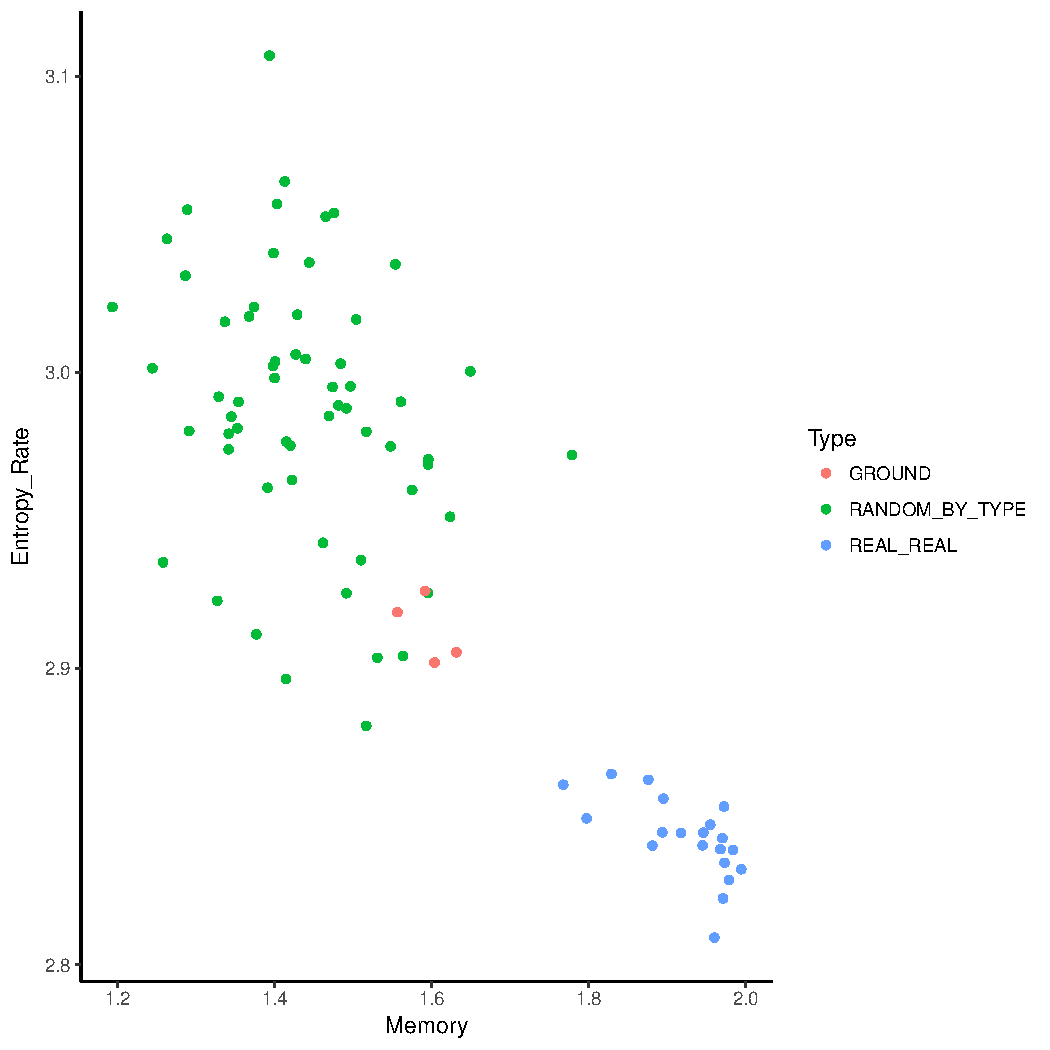
\includegraphics[width=0.25\textwidth]{figures/Afrikaans-entropy-memory.pdf}}  &  \multirow{4}{*}{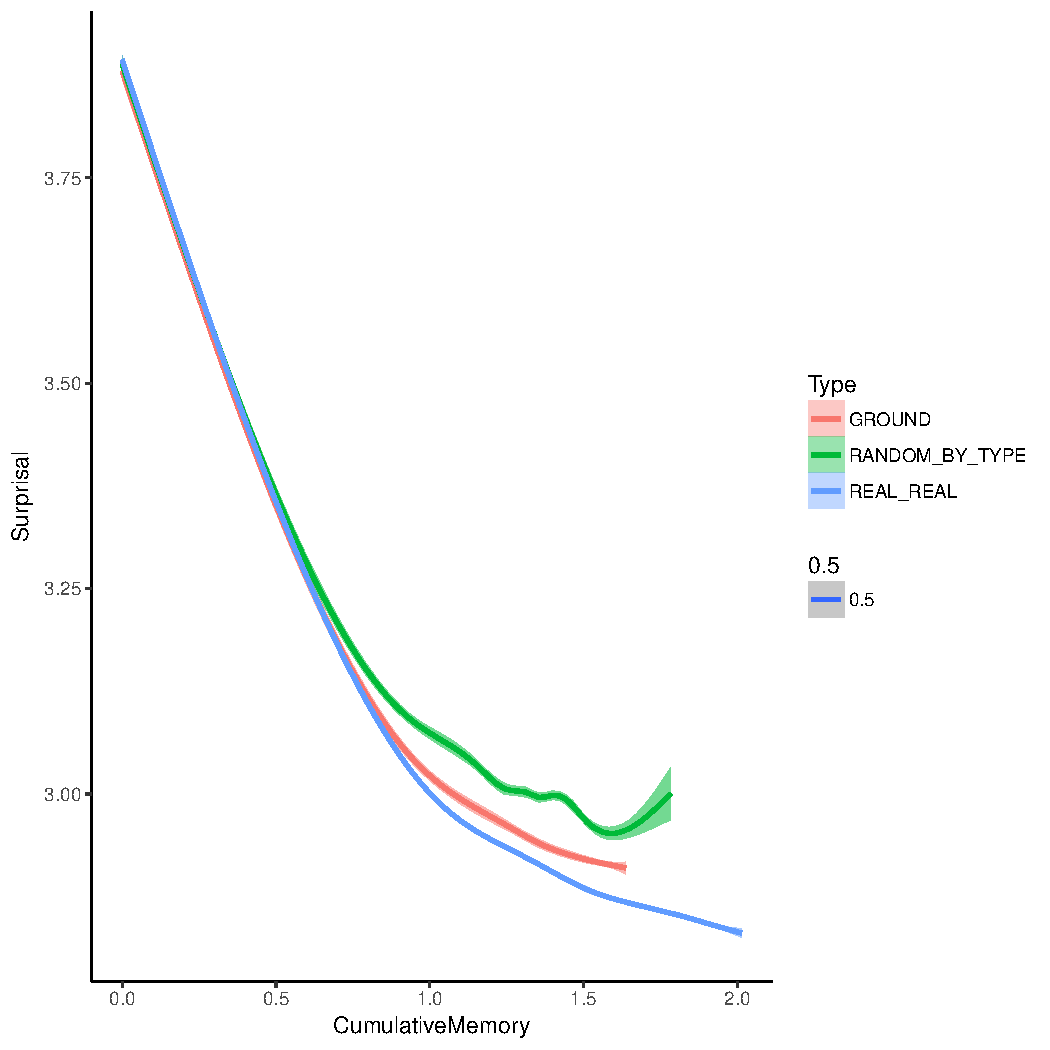
\includegraphics[width=0.25\textwidth]{figures/Afrikaans-listener-surprisal-memory.pdf}}  &  $D_x$  \\ 
  &    &    &  $W_x$  &  1.0  &  [1.0, 1.0]  \\ [10.25ex] \hline
Amharic-Adap  &  \multirow{4}{*}{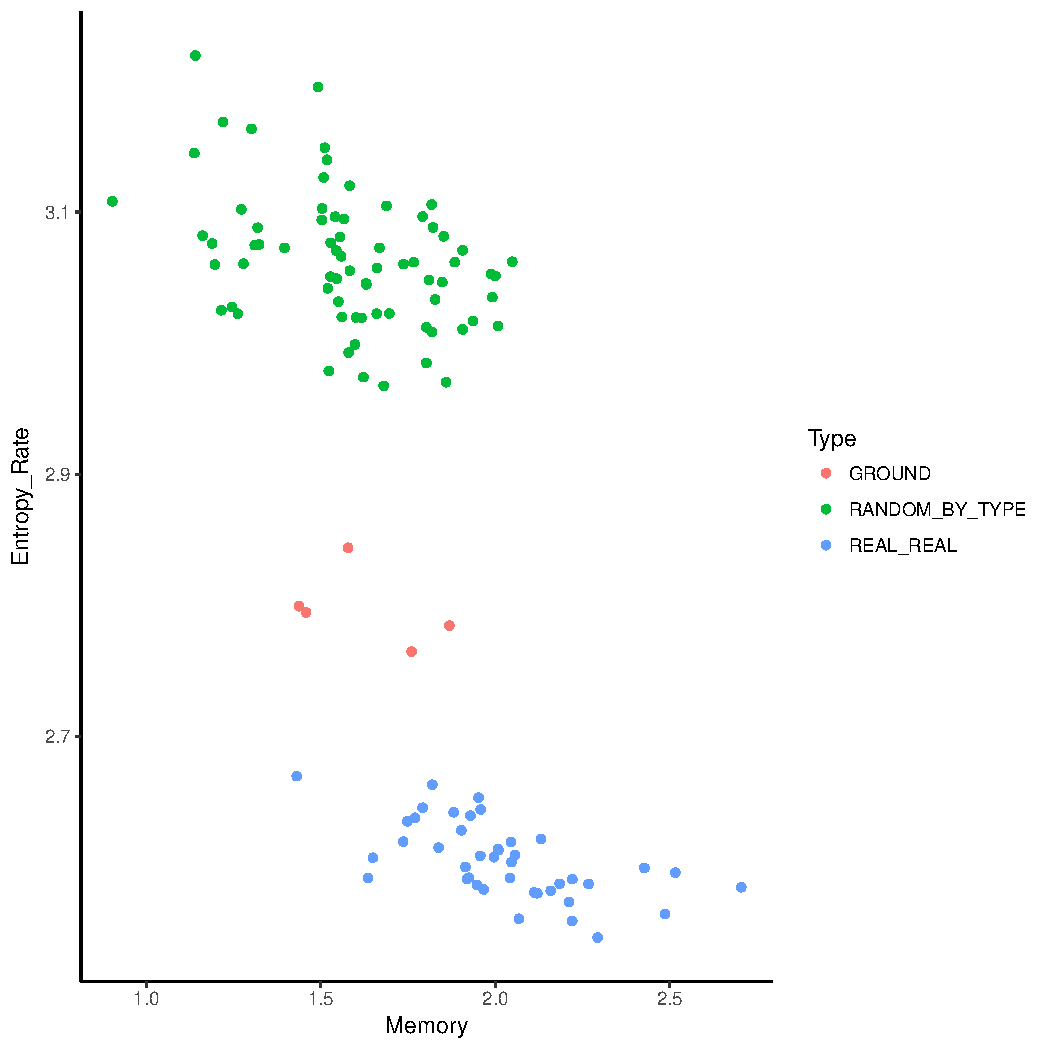
\includegraphics[width=0.25\textwidth]{figures/Amharic-Adap-entropy-memory.pdf}}  &  \multirow{4}{*}{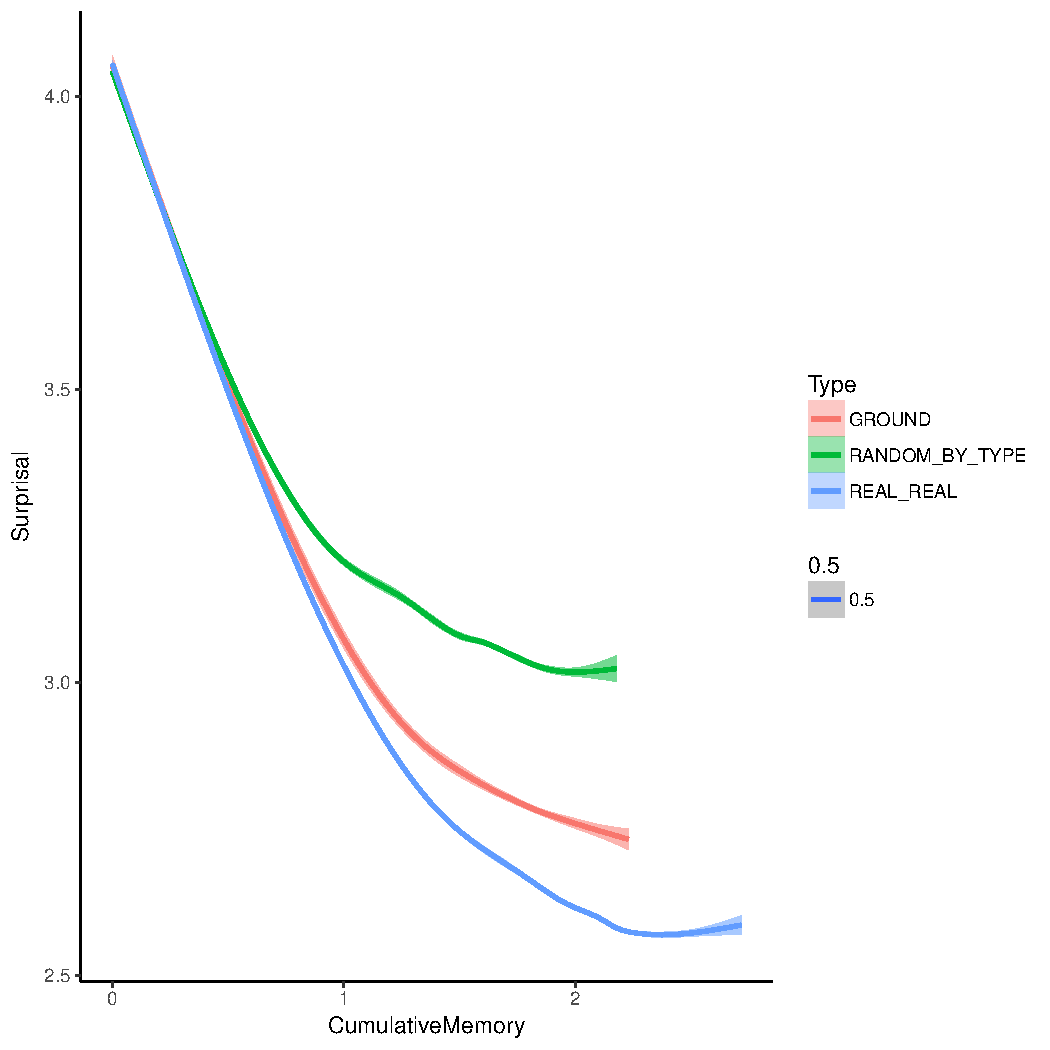
\includegraphics[width=0.25\textwidth]{figures/Amharic-Adap-listener-surprisal-memory.pdf}}  &  $D_x$  \\ 
  &    &    &  $W_x$  &  1.0  &  [1.0, 1.0]  \\ [10.25ex] \hline
Arabic  &  \multirow{4}{*}{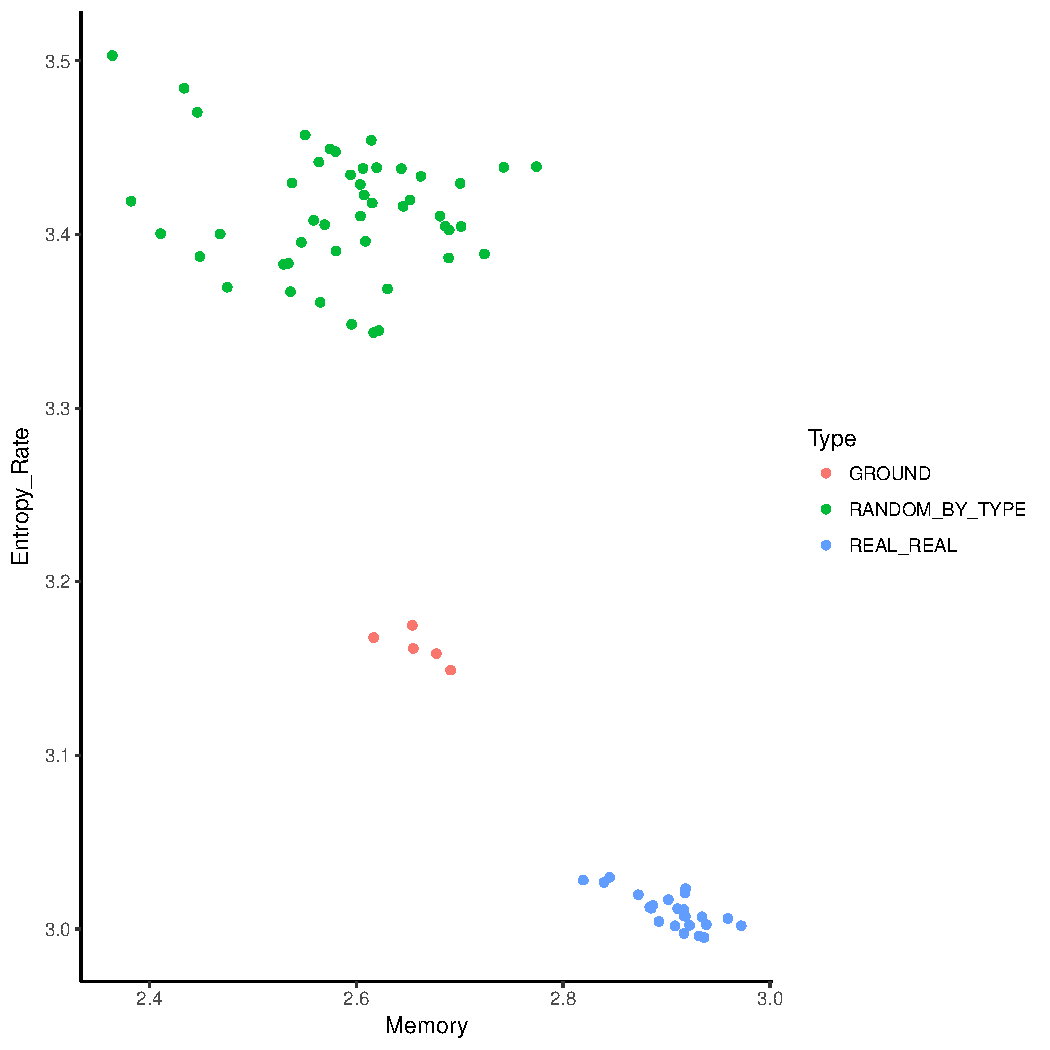
\includegraphics[width=0.25\textwidth]{figures/Arabic-entropy-memory.pdf}}  &  \multirow{4}{*}{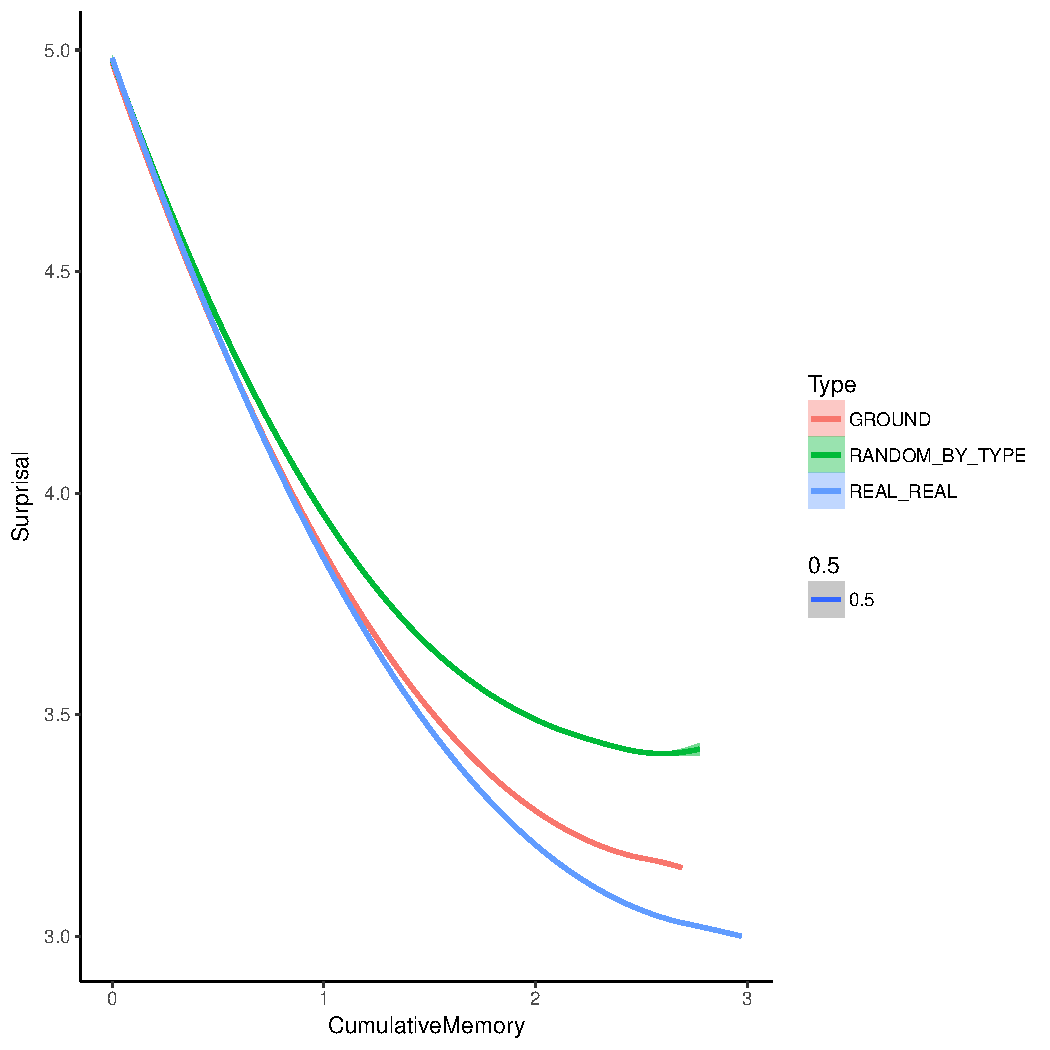
\includegraphics[width=0.25\textwidth]{figures/Arabic-listener-surprisal-memory.pdf}}  &  $D_x$  \\ 
  &    &    &  $W_x$  &  1.0  &  [1.0, 1.0]  \\ [10.25ex] \hline
Armenian-Adap*  &  \multirow{4}{*}{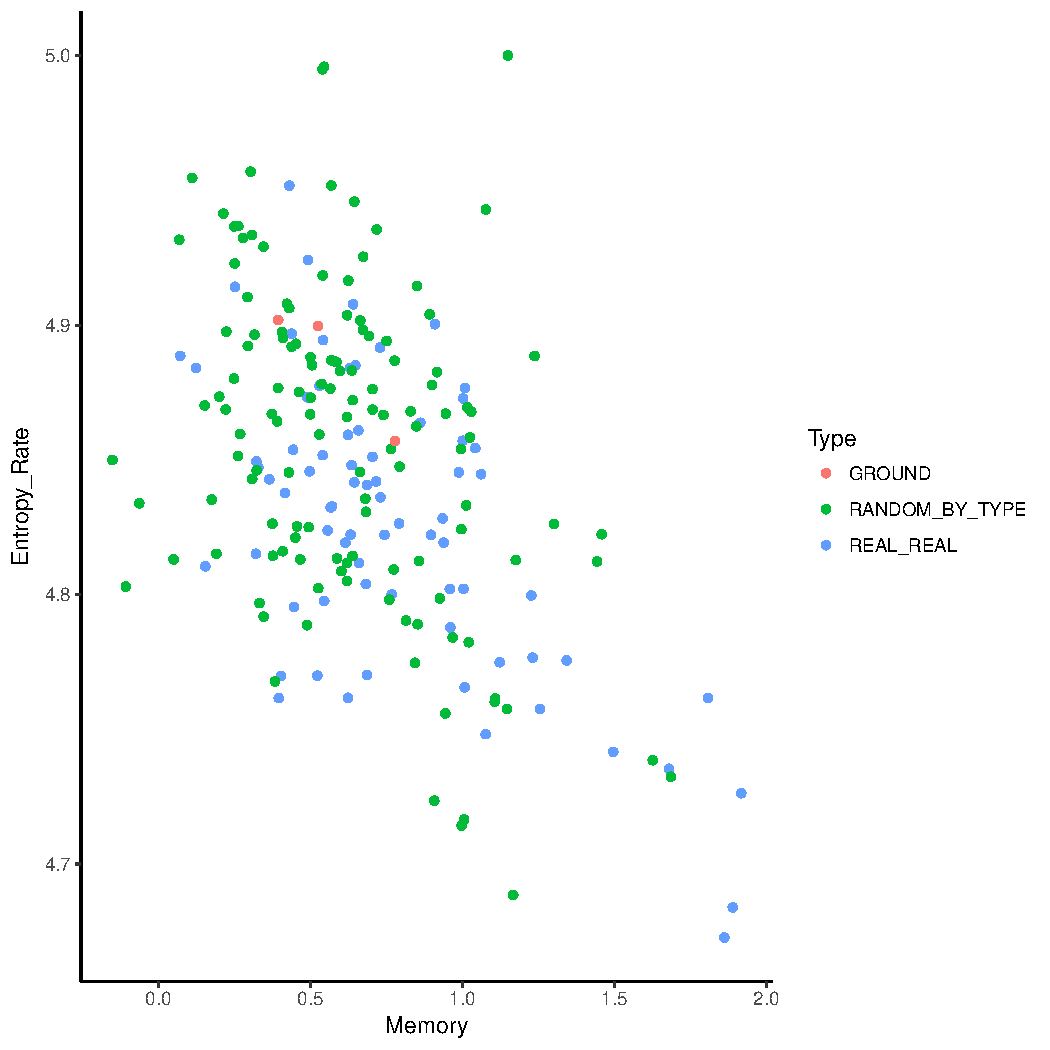
\includegraphics[width=0.25\textwidth]{figures/Armenian-Adap-entropy-memory.pdf}}  &  \multirow{4}{*}{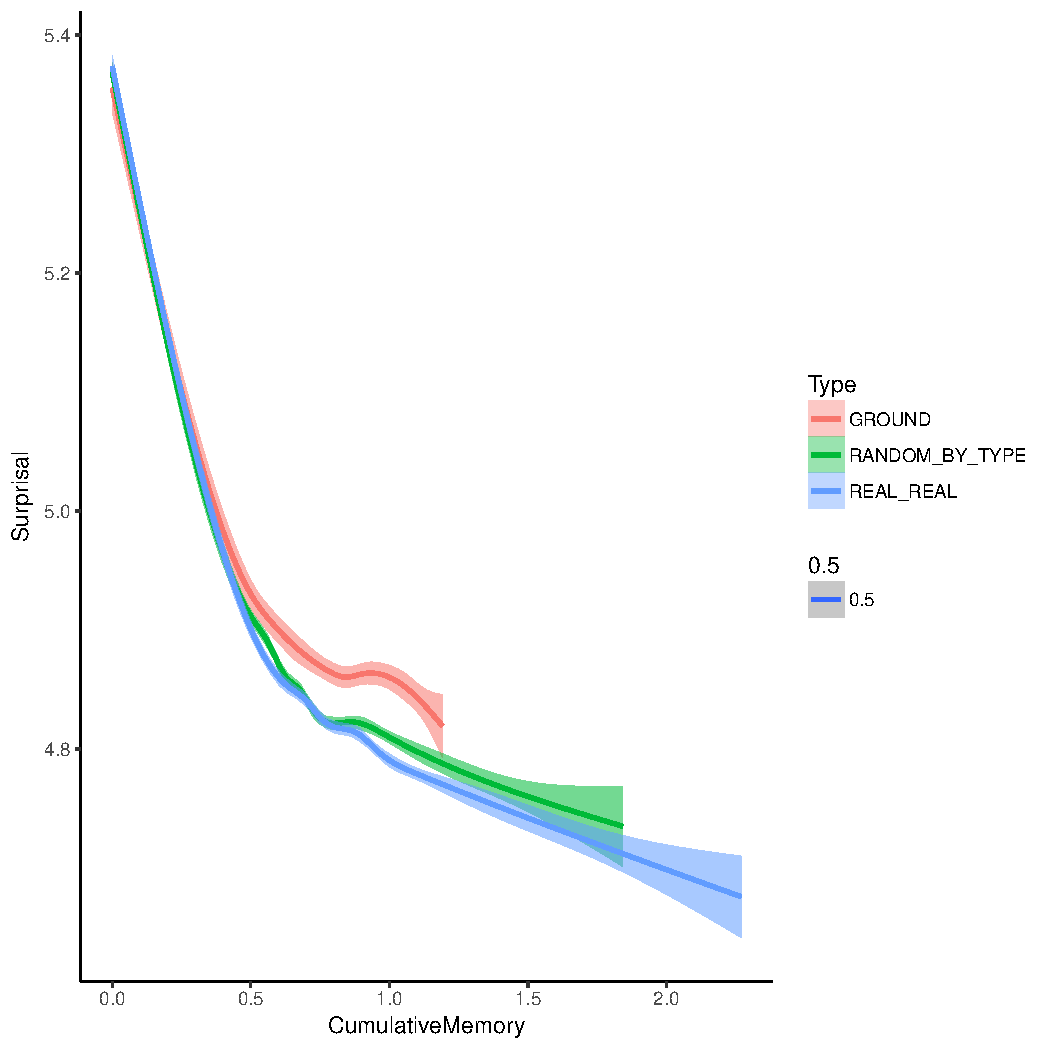
\includegraphics[width=0.25\textwidth]{figures/Armenian-Adap-listener-surprisal-memory.pdf}}  &  $D_x$  \\ 
  &    &    &  $W_x$  &  0.91  &  [0.83, 0.98]  \\ [10.25ex] \hline
Bambara-Adap  &  \multirow{4}{*}{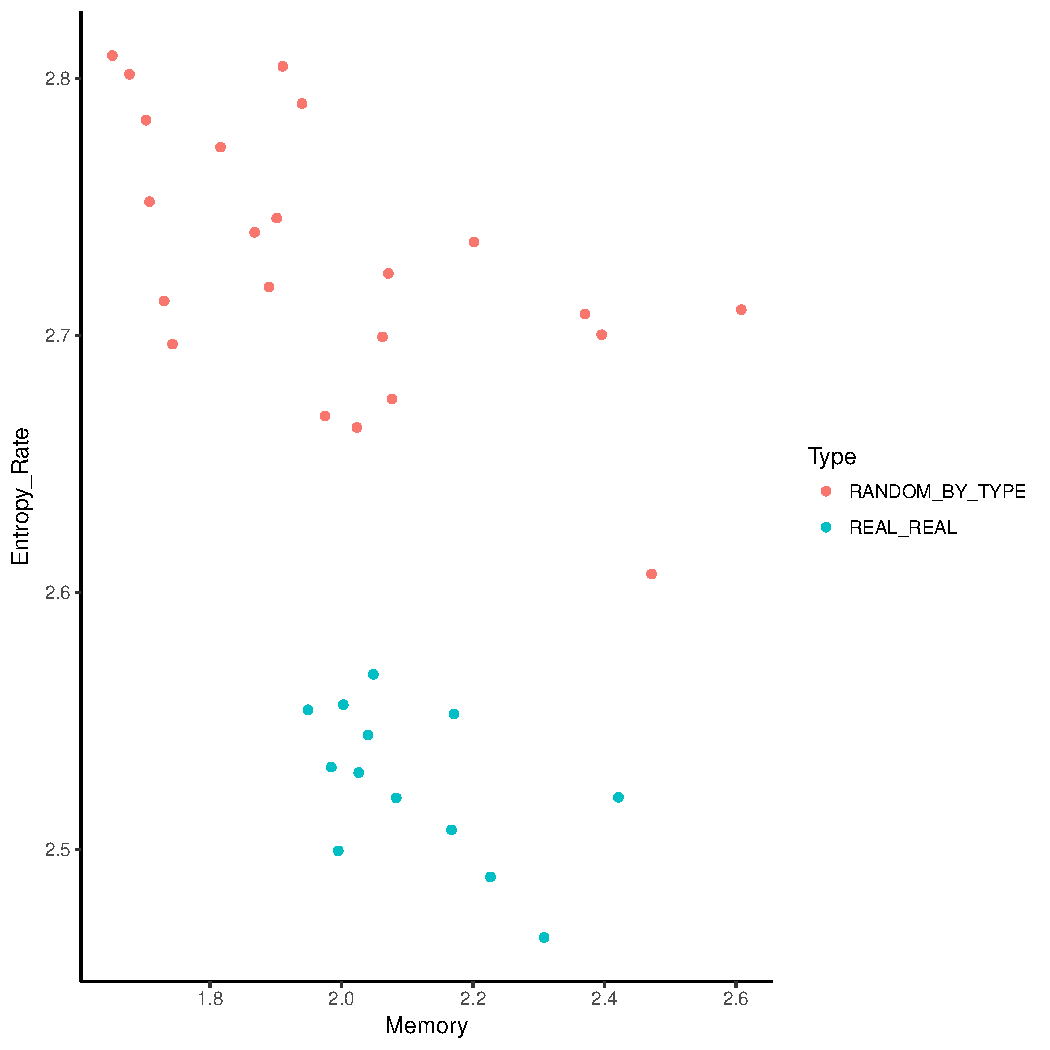
\includegraphics[width=0.25\textwidth]{figures/Bambara-Adap-entropy-memory.pdf}}  &  \multirow{4}{*}{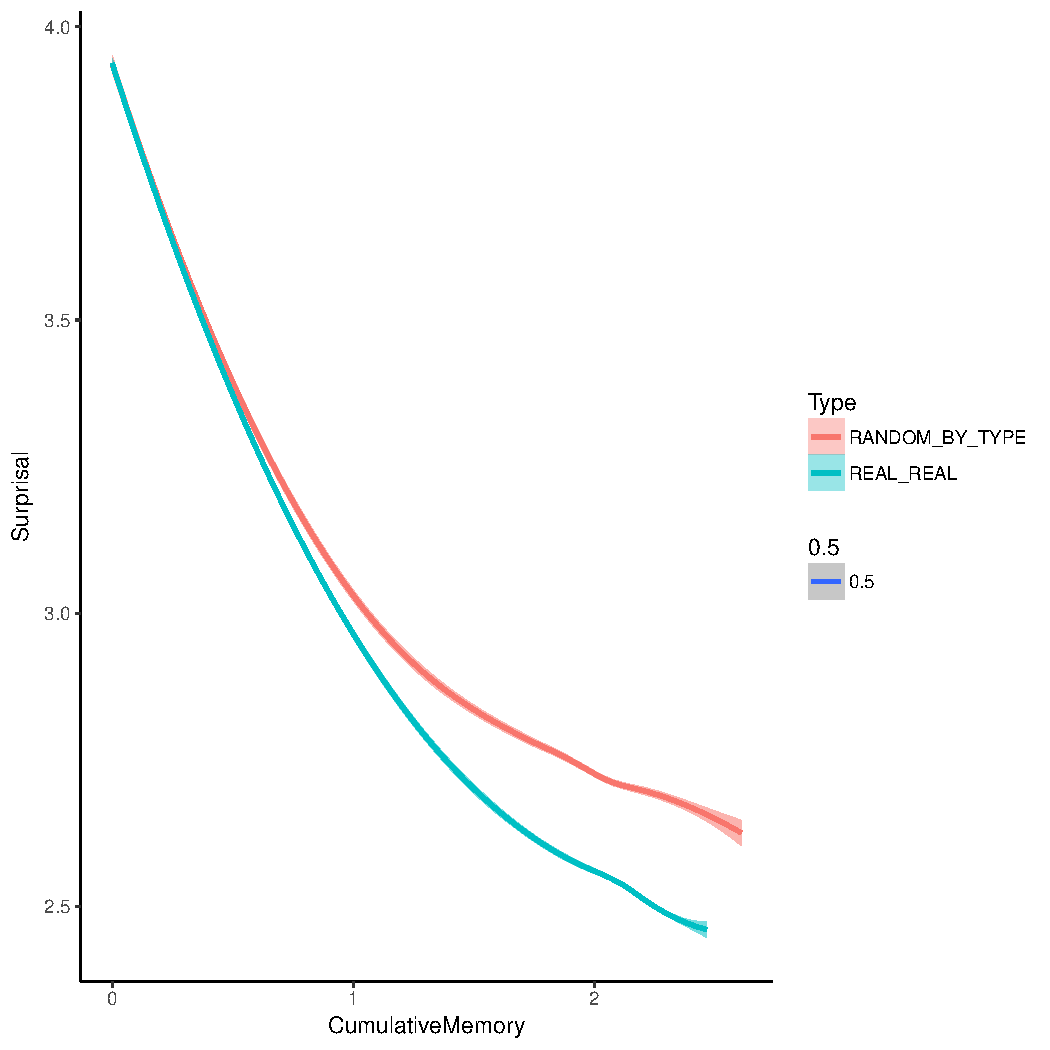
\includegraphics[width=0.25\textwidth]{figures/Bambara-Adap-listener-surprisal-memory.pdf}}  &  $D_x$  \\ 
  &    &    &  $W_x$  &  1.0  &  [1.0, 1.0]  \\ [10.25ex] \hline
Basque  &  \multirow{4}{*}{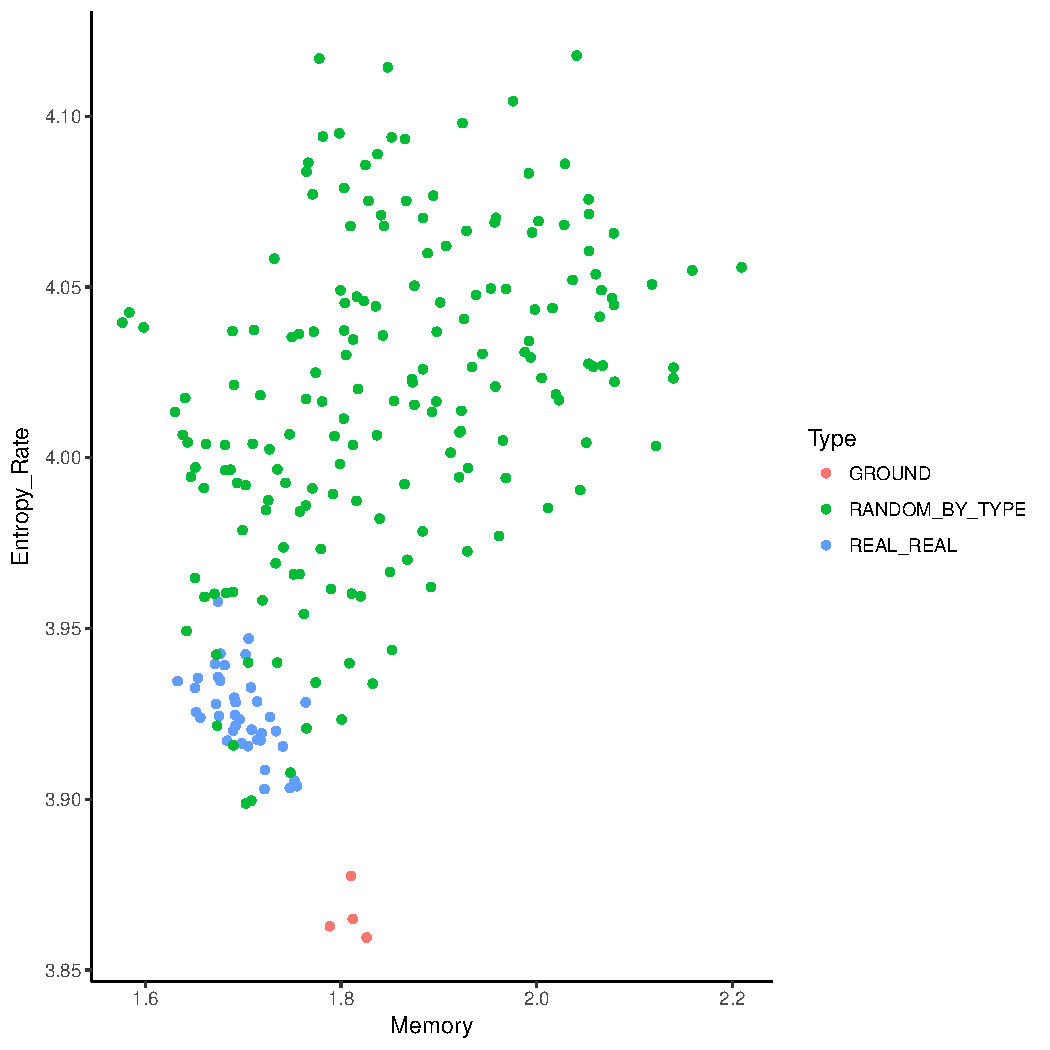
\includegraphics[width=0.25\textwidth]{figures/Basque-entropy-memory.pdf}}  &  \multirow{4}{*}{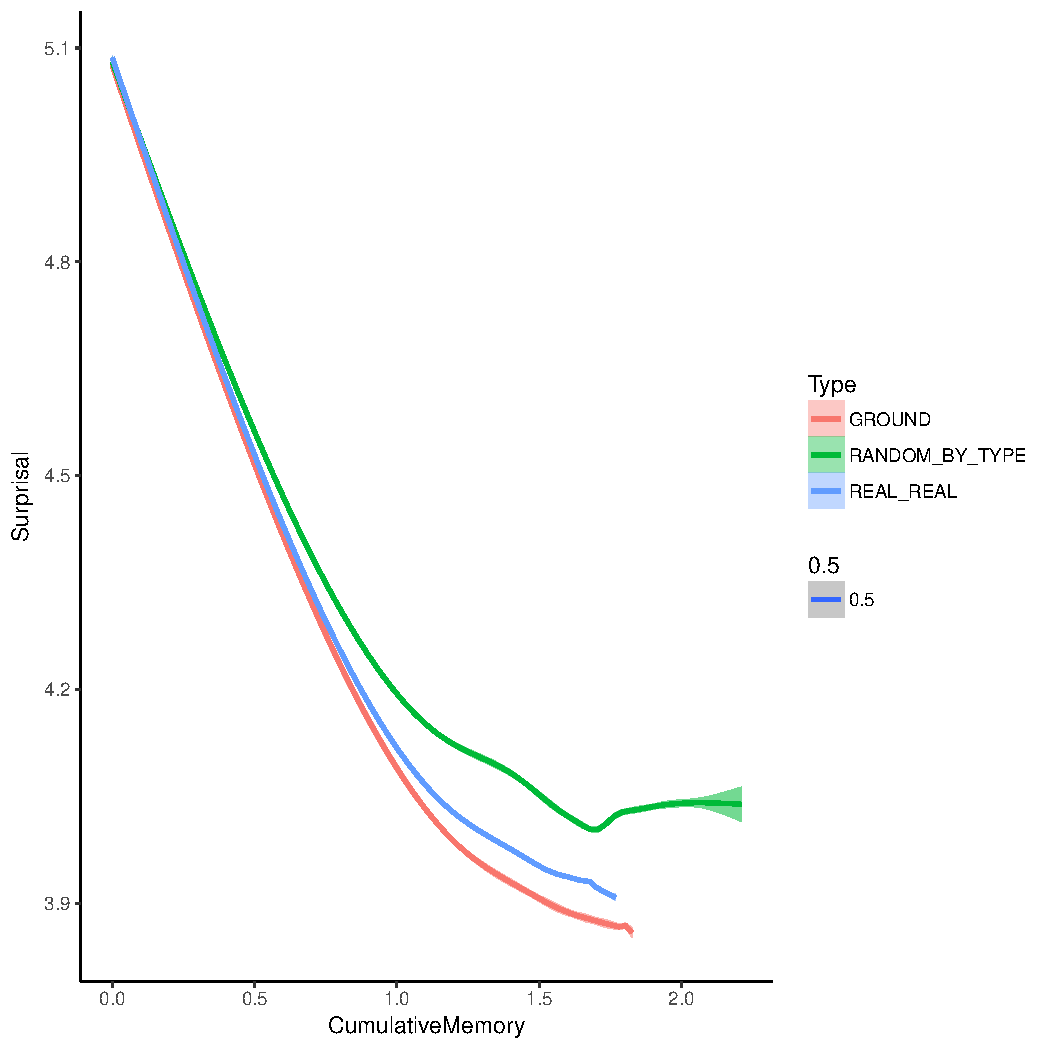
\includegraphics[width=0.25\textwidth]{figures/Basque-listener-surprisal-memory.pdf}}  &  $D_x$  \\ 
  &    &    &  $W_x$  &  1.0  &  [1.0, 1.0]  \\ [10.25ex] \hline
Breton-Adap  &  \multirow{4}{*}{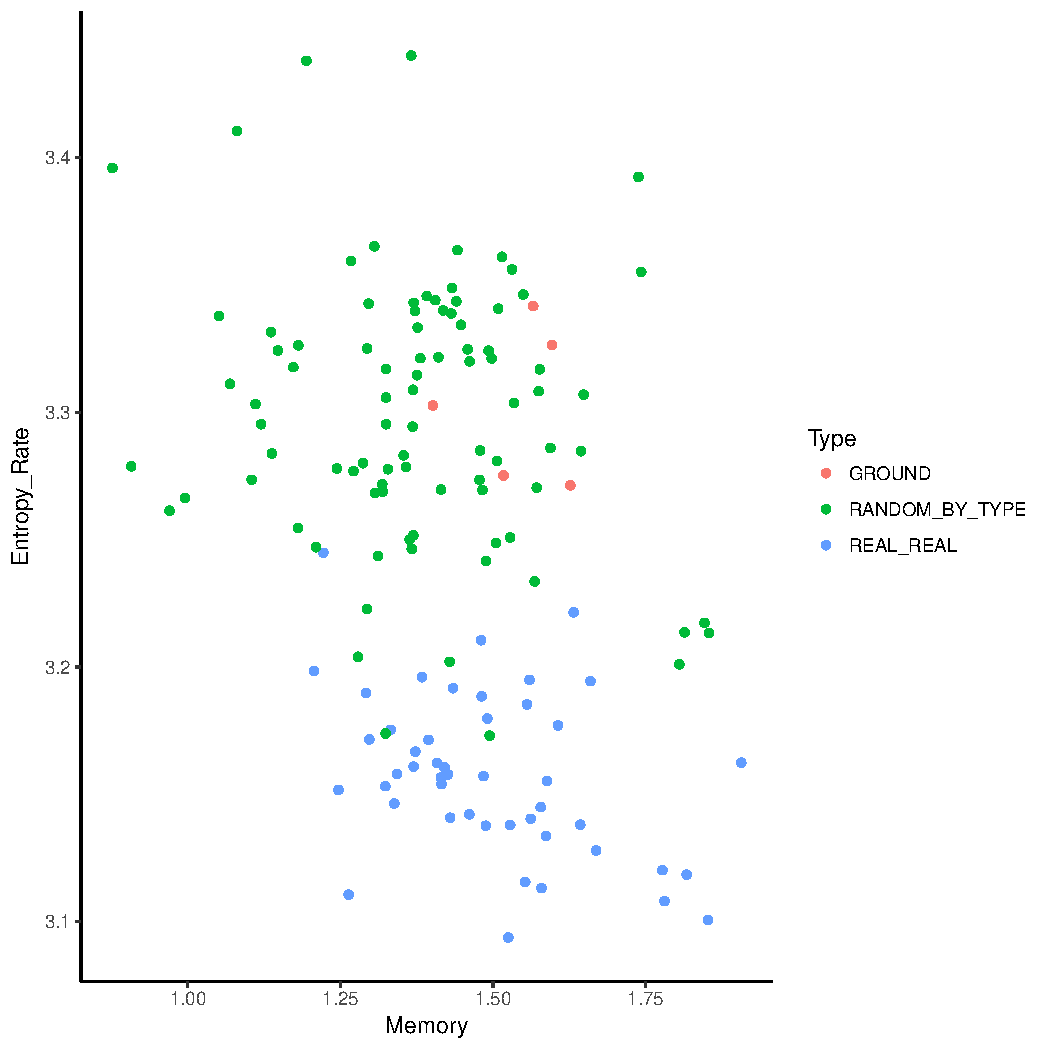
\includegraphics[width=0.25\textwidth]{figures/Breton-Adap-entropy-memory.pdf}}  &  \multirow{4}{*}{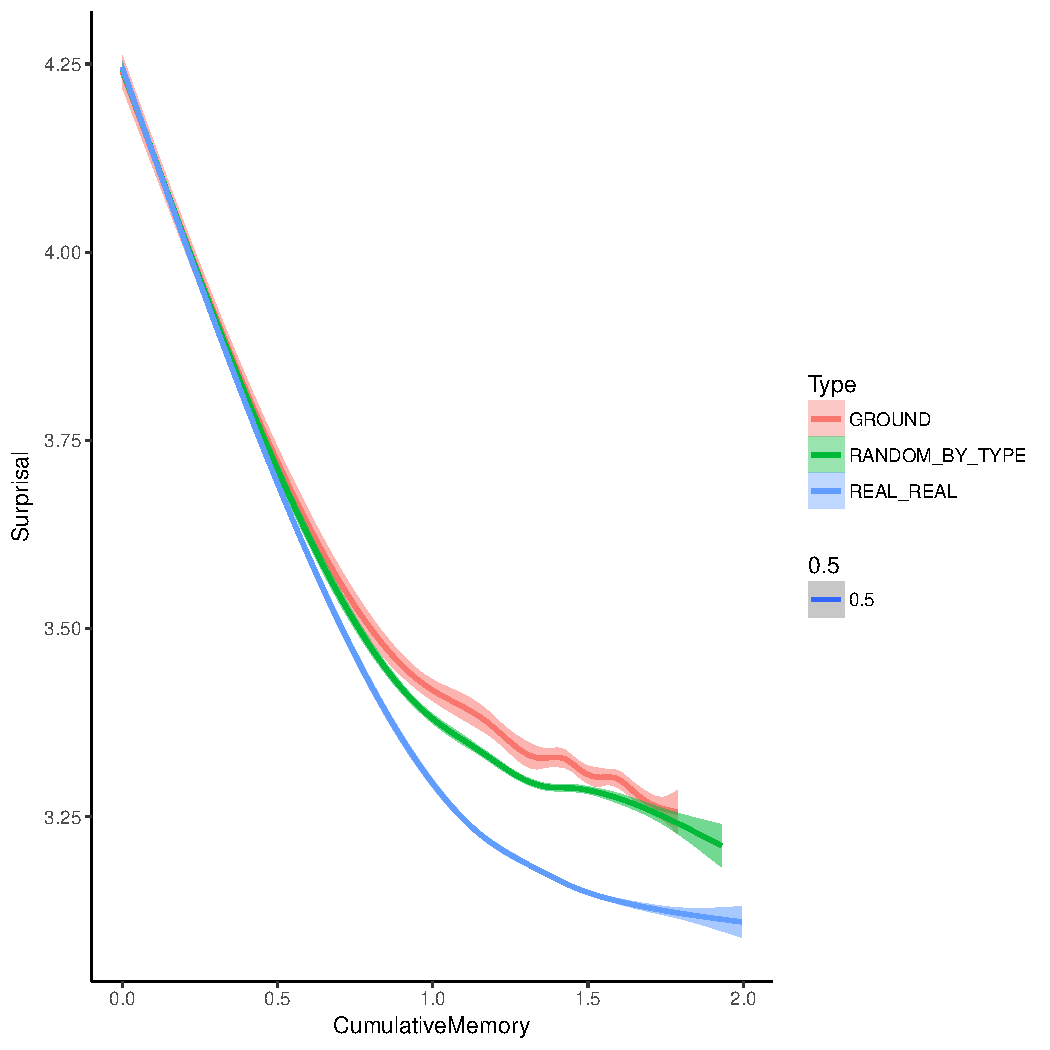
\includegraphics[width=0.25\textwidth]{figures/Breton-Adap-listener-surprisal-memory.pdf}}  &  $D_x$  \\ 
  &    &    &  $W_x$  &  1.0  &  [1.0, 1.0]  \\ [10.25ex] \hline
Bulgarian  &  \multirow{4}{*}{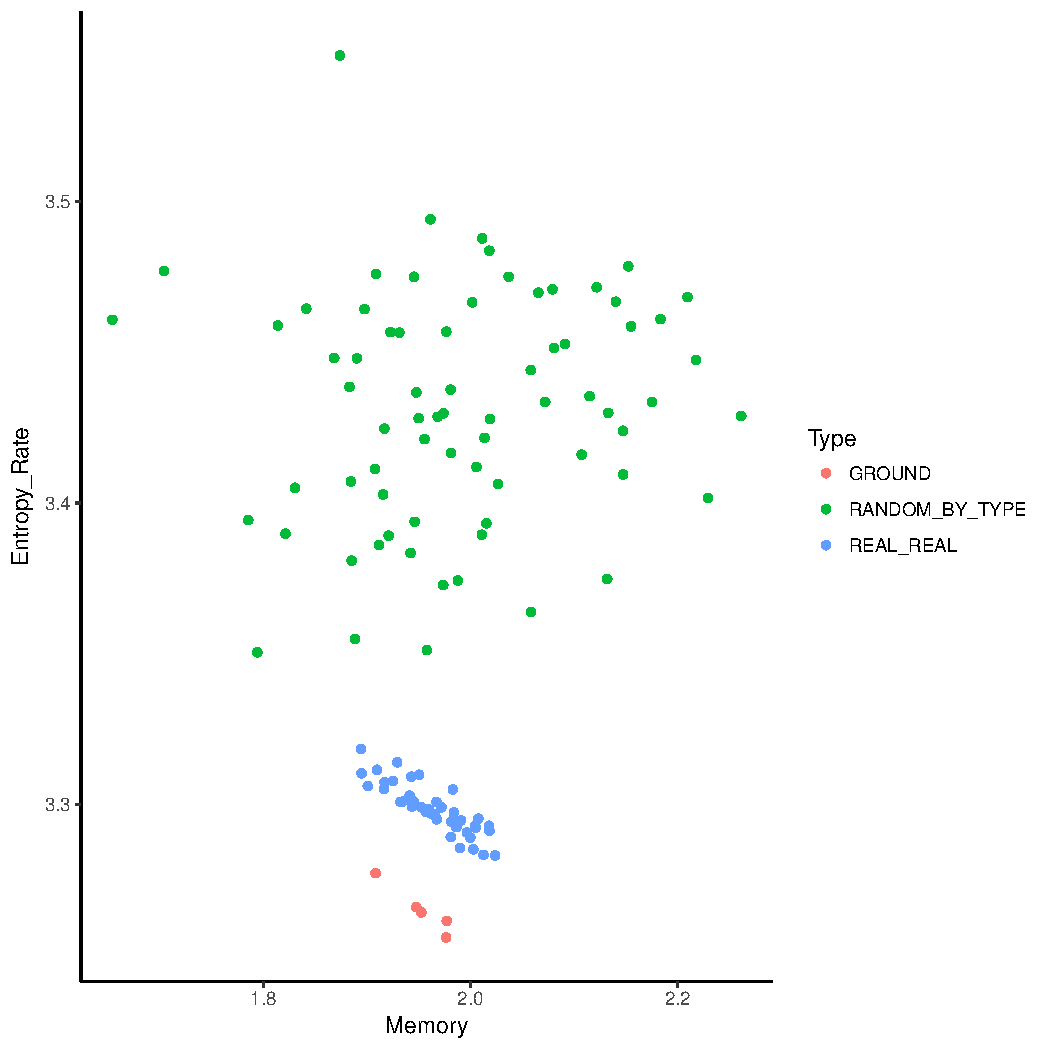
\includegraphics[width=0.25\textwidth]{figures/Bulgarian-entropy-memory.pdf}}  &  \multirow{4}{*}{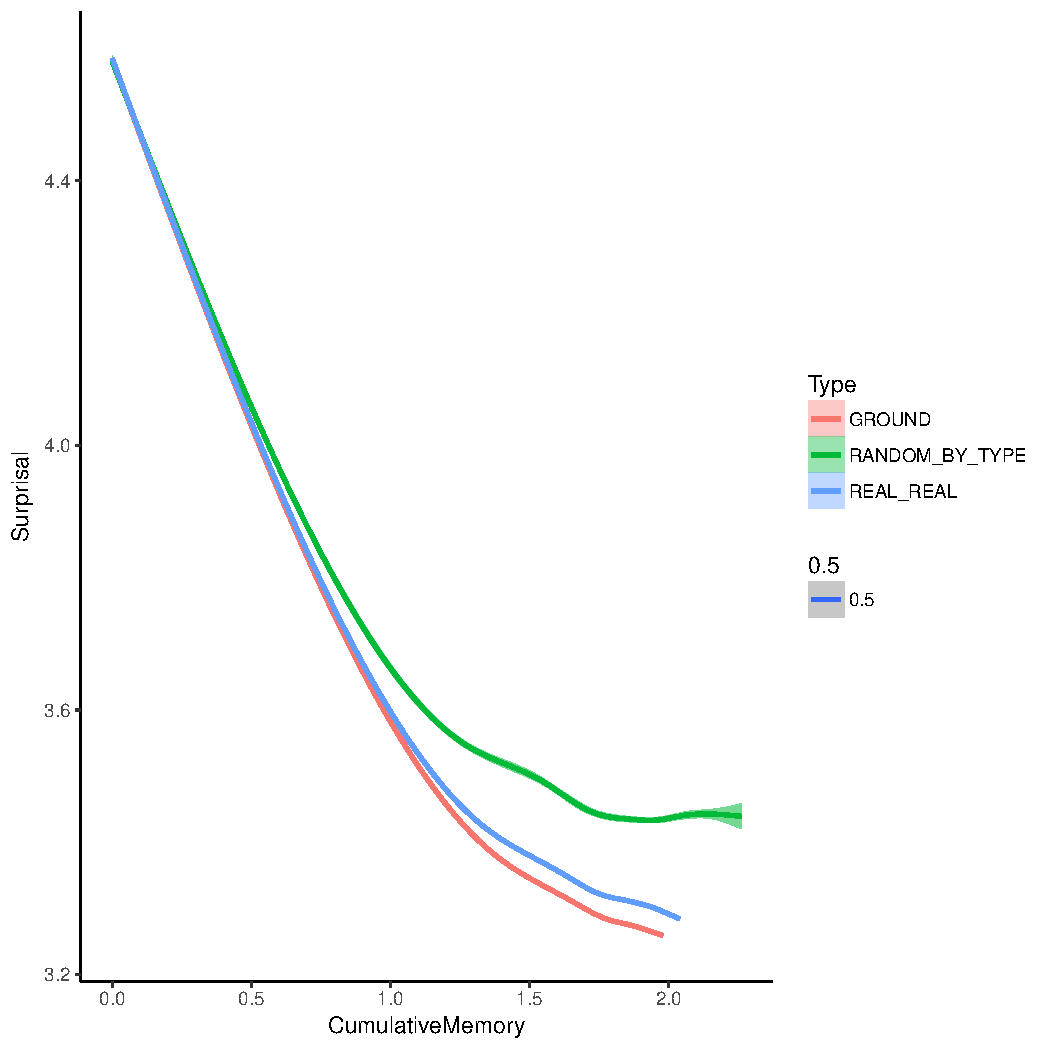
\includegraphics[width=0.25\textwidth]{figures/Bulgarian-listener-surprisal-memory.pdf}}  &  $D_x$  \\ 
  &    &    &  $W_x$  &  1.0  &  [1.0, 1.0]  \\ [10.25ex] \hline
Buryat-Adap  &  \multirow{4}{*}{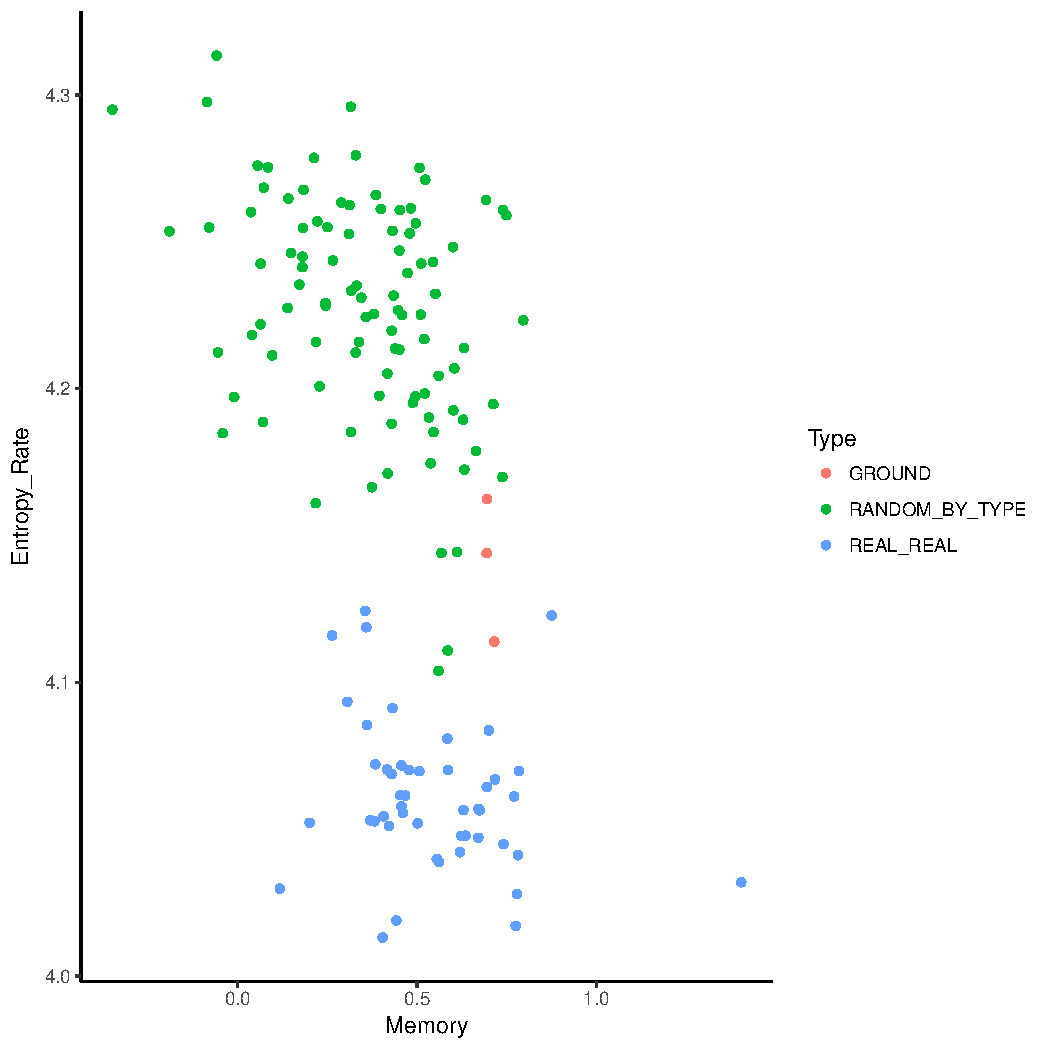
\includegraphics[width=0.25\textwidth]{figures/Buryat-Adap-entropy-memory.pdf}}  &  \multirow{4}{*}{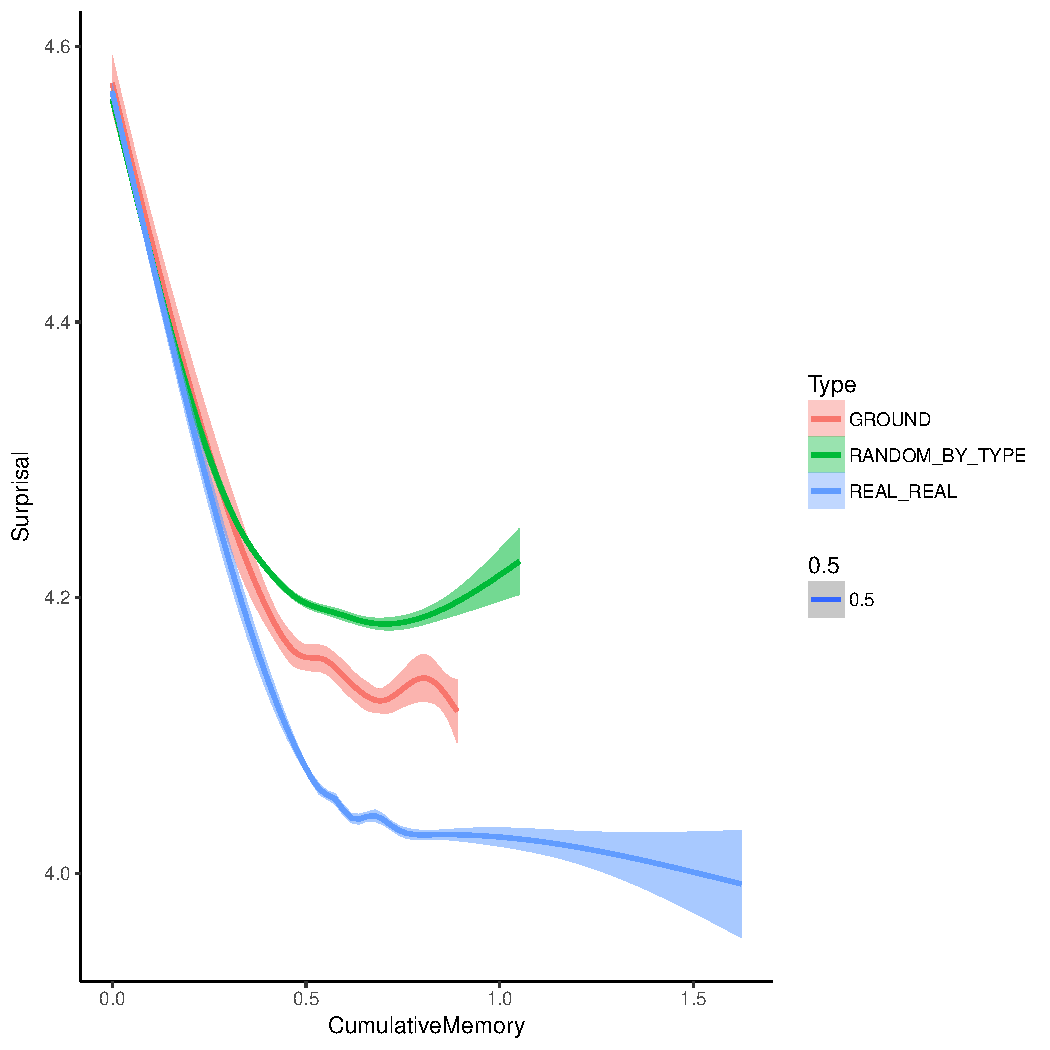
\includegraphics[width=0.25\textwidth]{figures/Buryat-Adap-listener-surprisal-memory.pdf}}  &  $D_x$  \\ 
  &    &    &  $W_x$  &  1.0  &  [1.0, 1.0]  \\ [10.25ex] \hline
Cantonese-Adap  &  \multirow{4}{*}{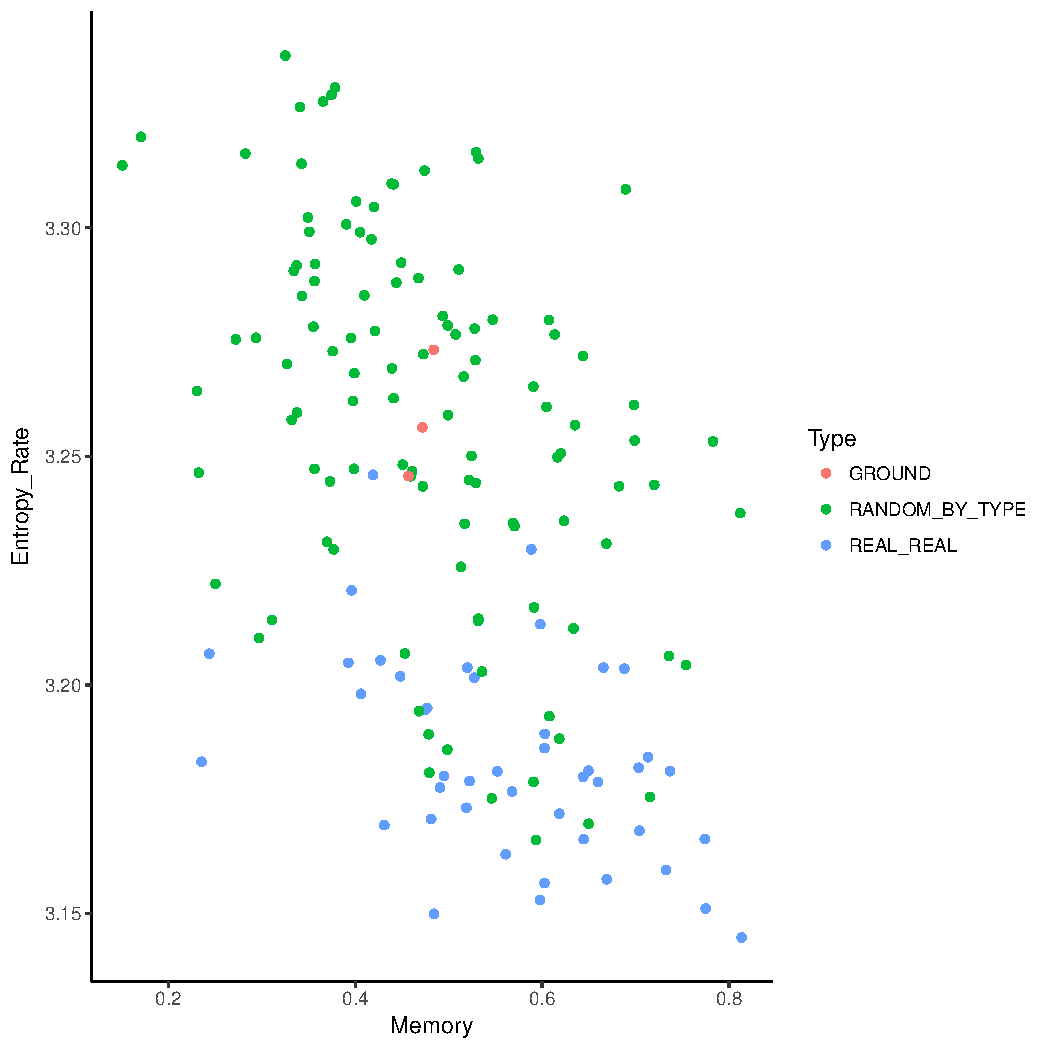
\includegraphics[width=0.25\textwidth]{figures/Cantonese-Adap-entropy-memory.pdf}}  &  \multirow{4}{*}{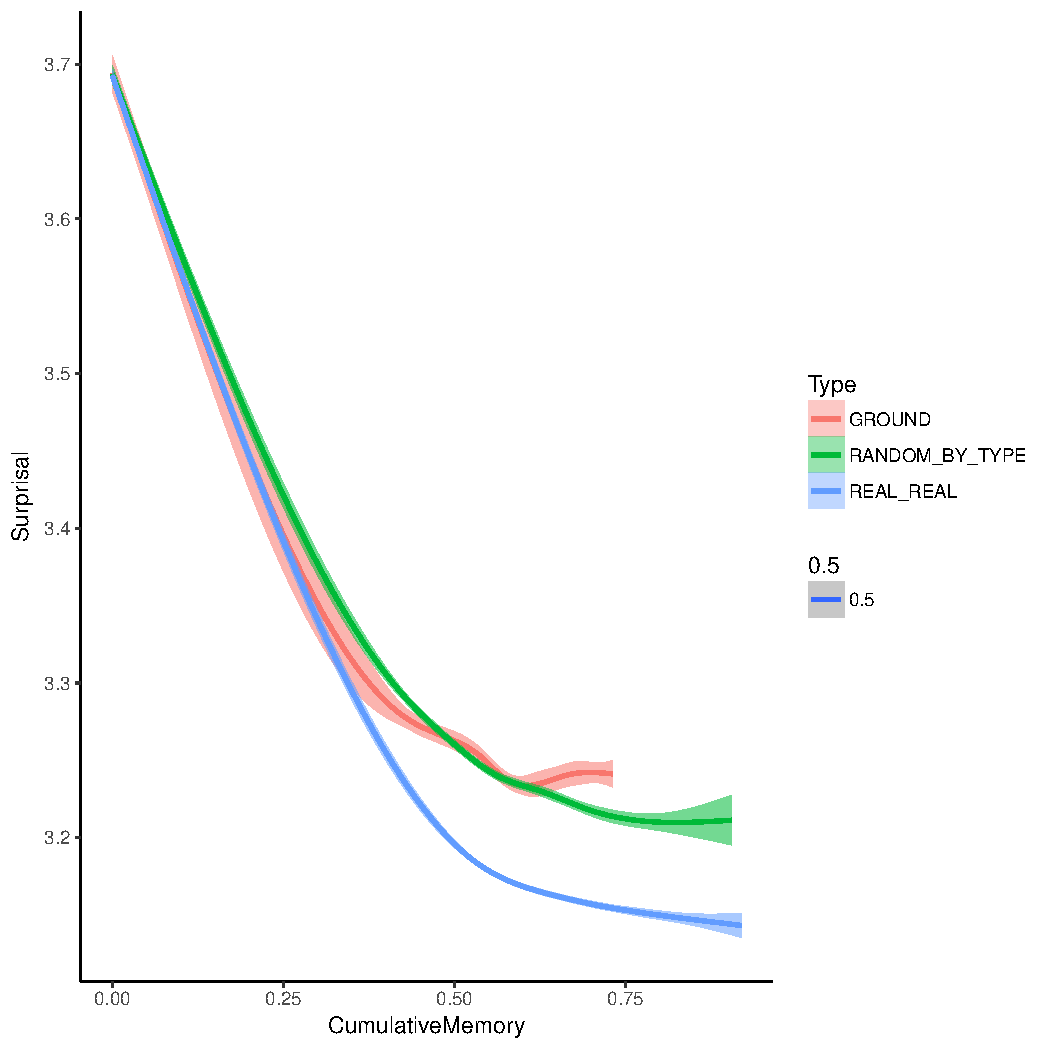
\includegraphics[width=0.25\textwidth]{figures/Cantonese-Adap-listener-surprisal-memory.pdf}}  &  $D_x$  \\ 
  &    &    &  $W_x$  &  0.96  &  [0.86, 1.0]  \\ [10.25ex] \hline
Catalan  &  \multirow{4}{*}{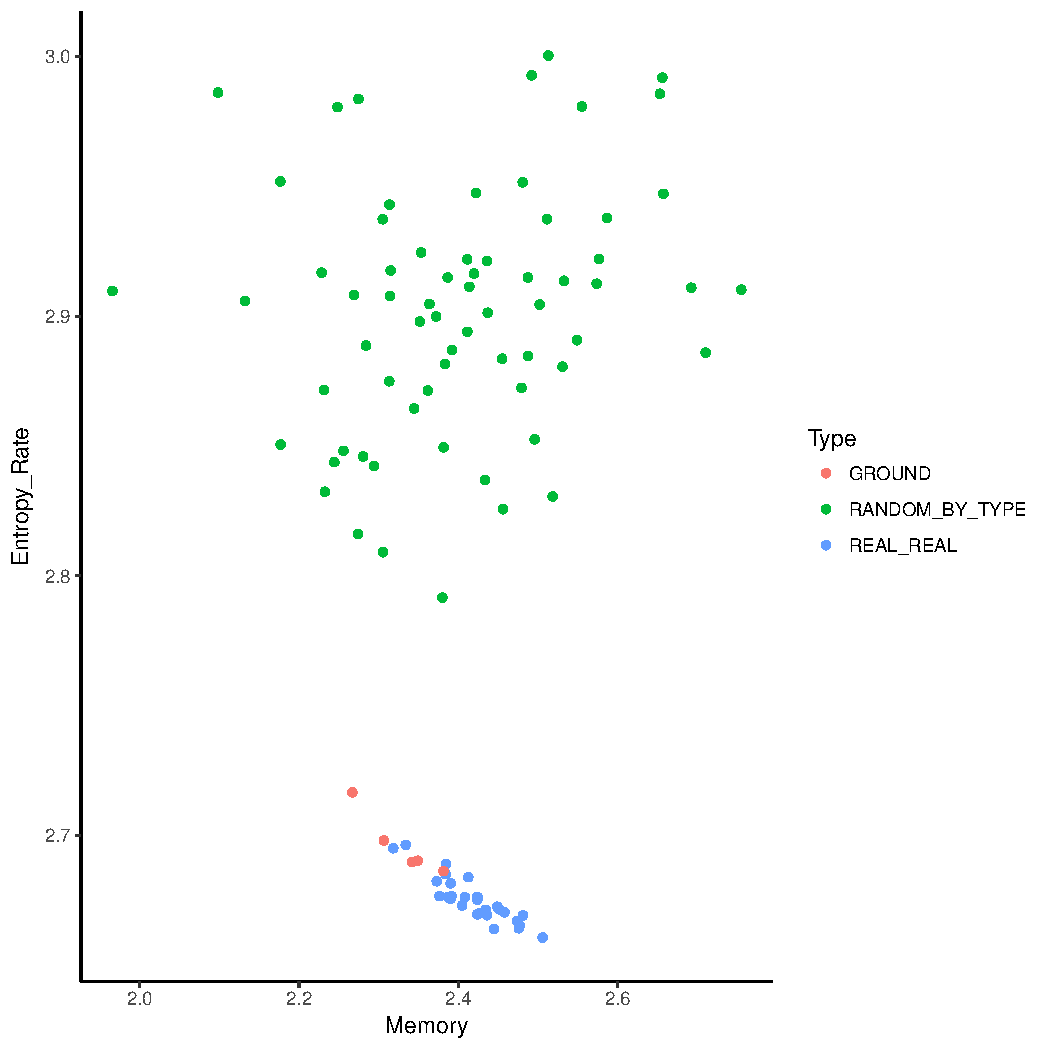
\includegraphics[width=0.25\textwidth]{figures/Catalan-entropy-memory.pdf}}  &  \multirow{4}{*}{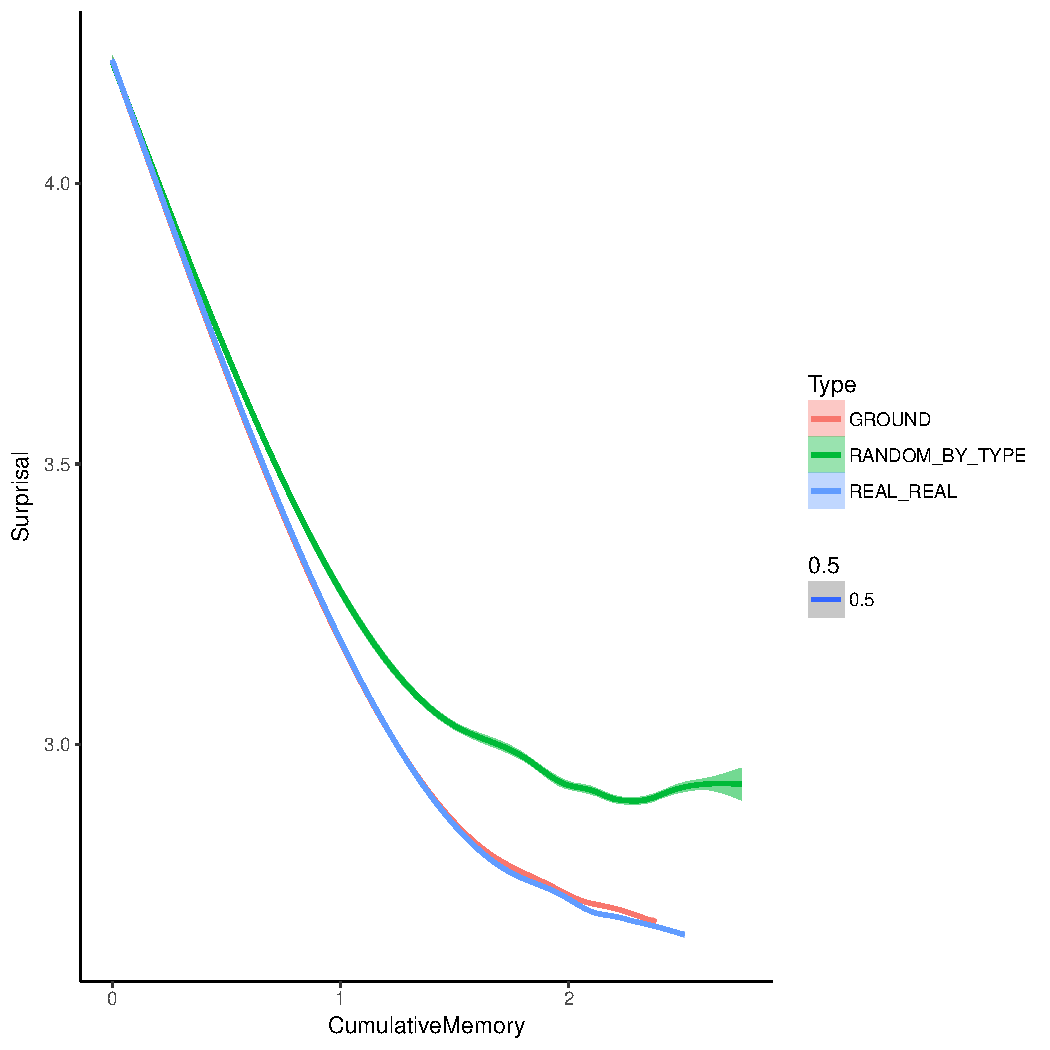
\includegraphics[width=0.25\textwidth]{figures/Catalan-listener-surprisal-memory.pdf}}  &  $D_x$  \\ 
  &    &    &  $W_x$  &  1.0  &  [1.0, 1.0]  \\ [10.25ex] \hline
Chinese  &  \multirow{4}{*}{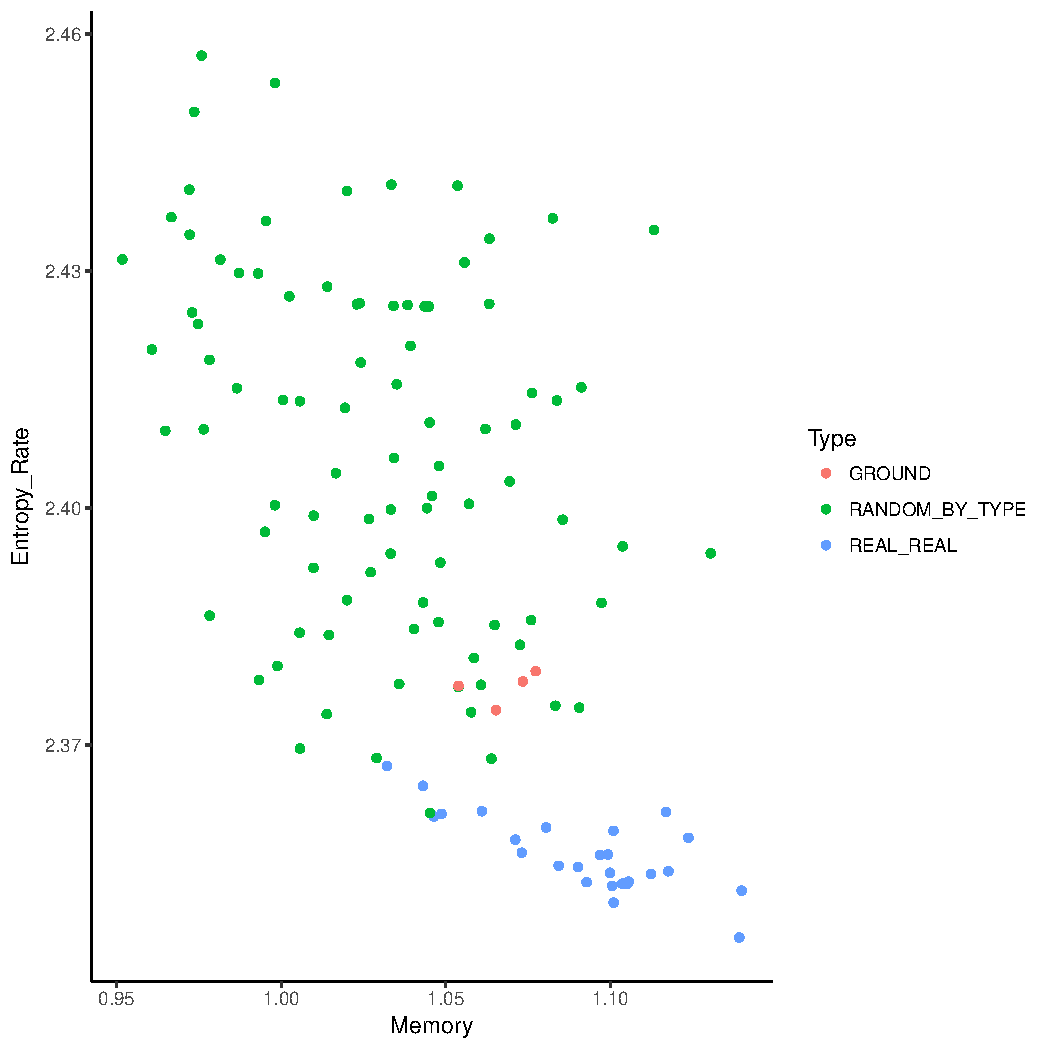
\includegraphics[width=0.25\textwidth]{figures/Chinese-entropy-memory.pdf}}  &  \multirow{4}{*}{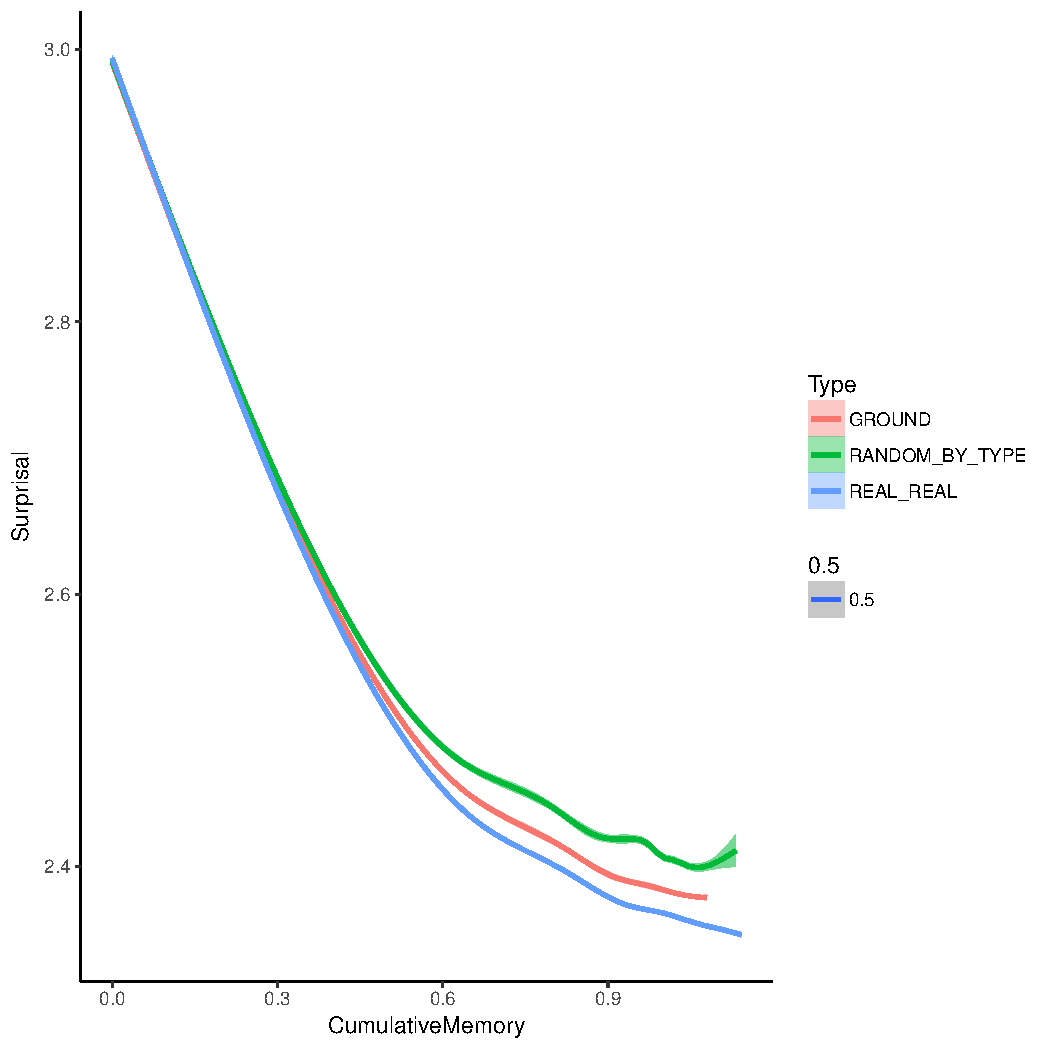
\includegraphics[width=0.25\textwidth]{figures/Chinese-listener-surprisal-memory.pdf}}  &  $D_x$  \\ 
  &    &    &  $W_x$  &  1.0  &  [1.0, 1.0]  \\ [10.25ex] \hline
Croatian  &  \multirow{4}{*}{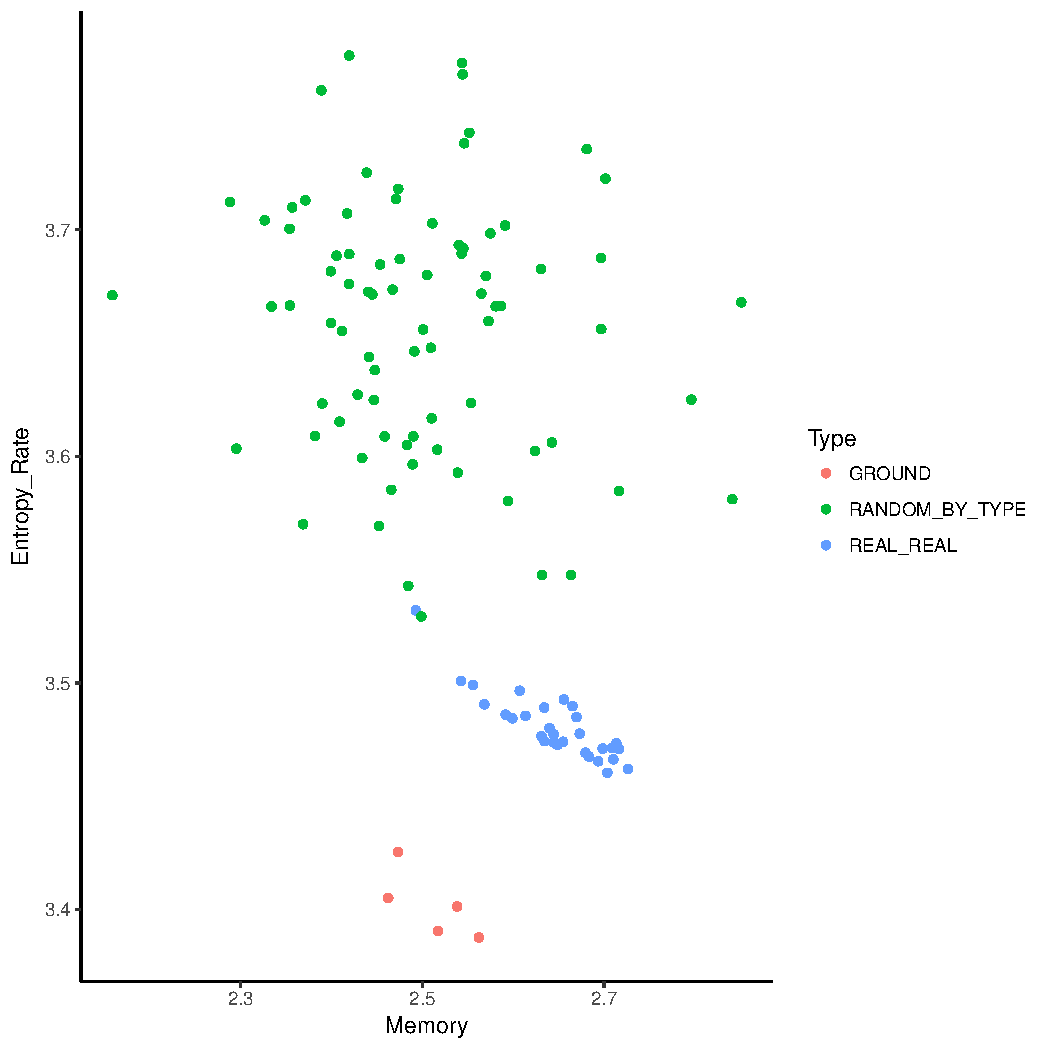
\includegraphics[width=0.25\textwidth]{figures/Croatian-entropy-memory.pdf}}  &  \multirow{4}{*}{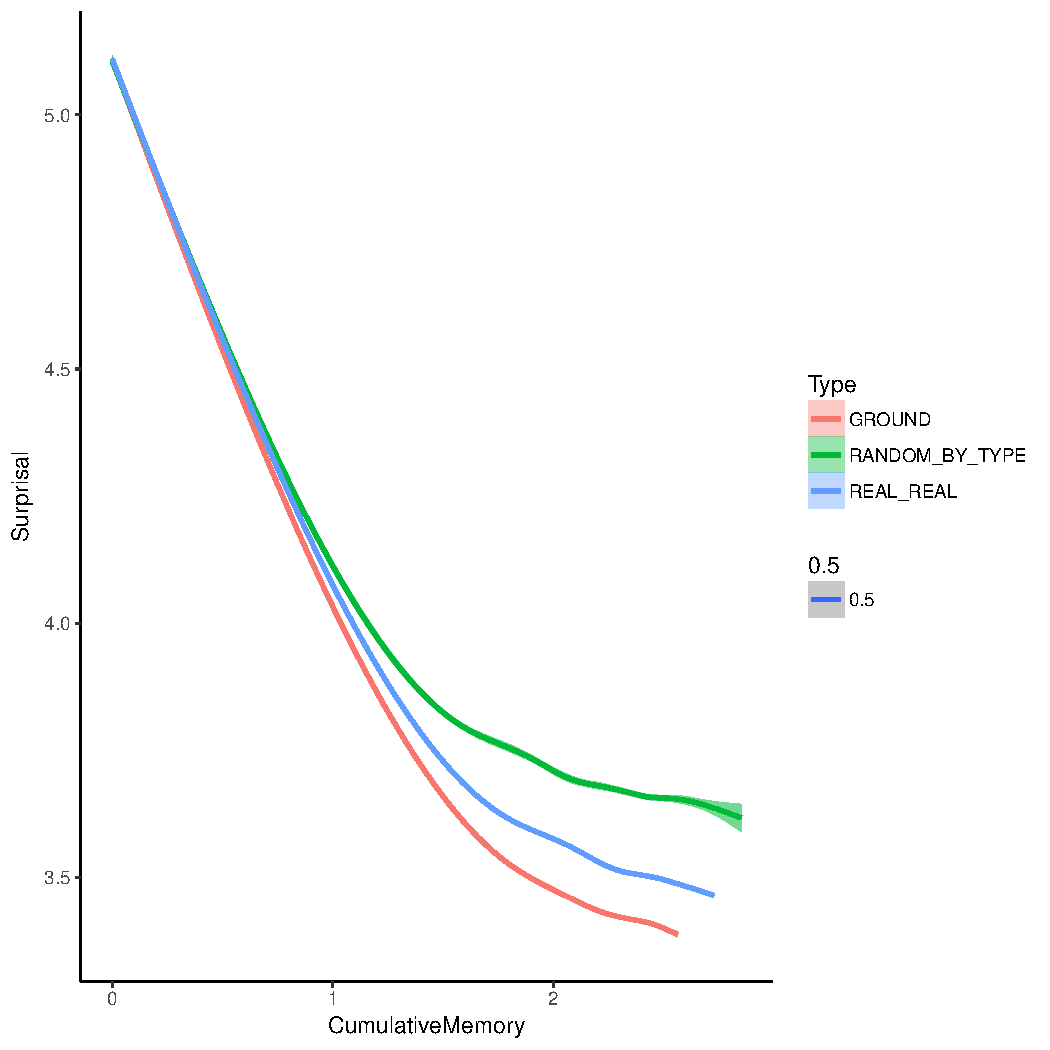
\includegraphics[width=0.25\textwidth]{figures/Croatian-listener-surprisal-memory.pdf}}  &  $D_x$  \\ 
  &    &    &  $W_x$  &  1.0  &  [1.0, 1.0]  \\ [10.25ex] \hline
Czech  &  \multirow{4}{*}{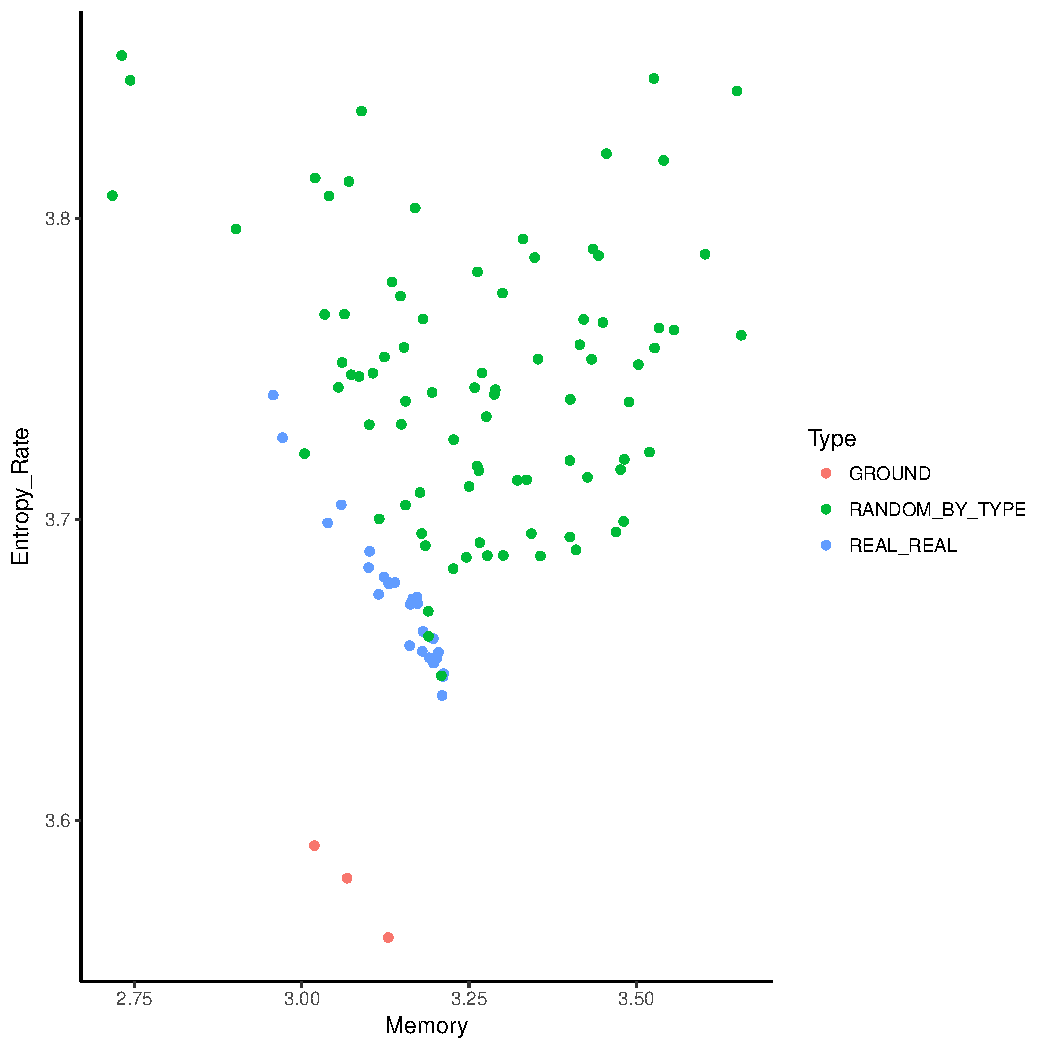
\includegraphics[width=0.25\textwidth]{figures/Czech-entropy-memory.pdf}}  &  \multirow{4}{*}{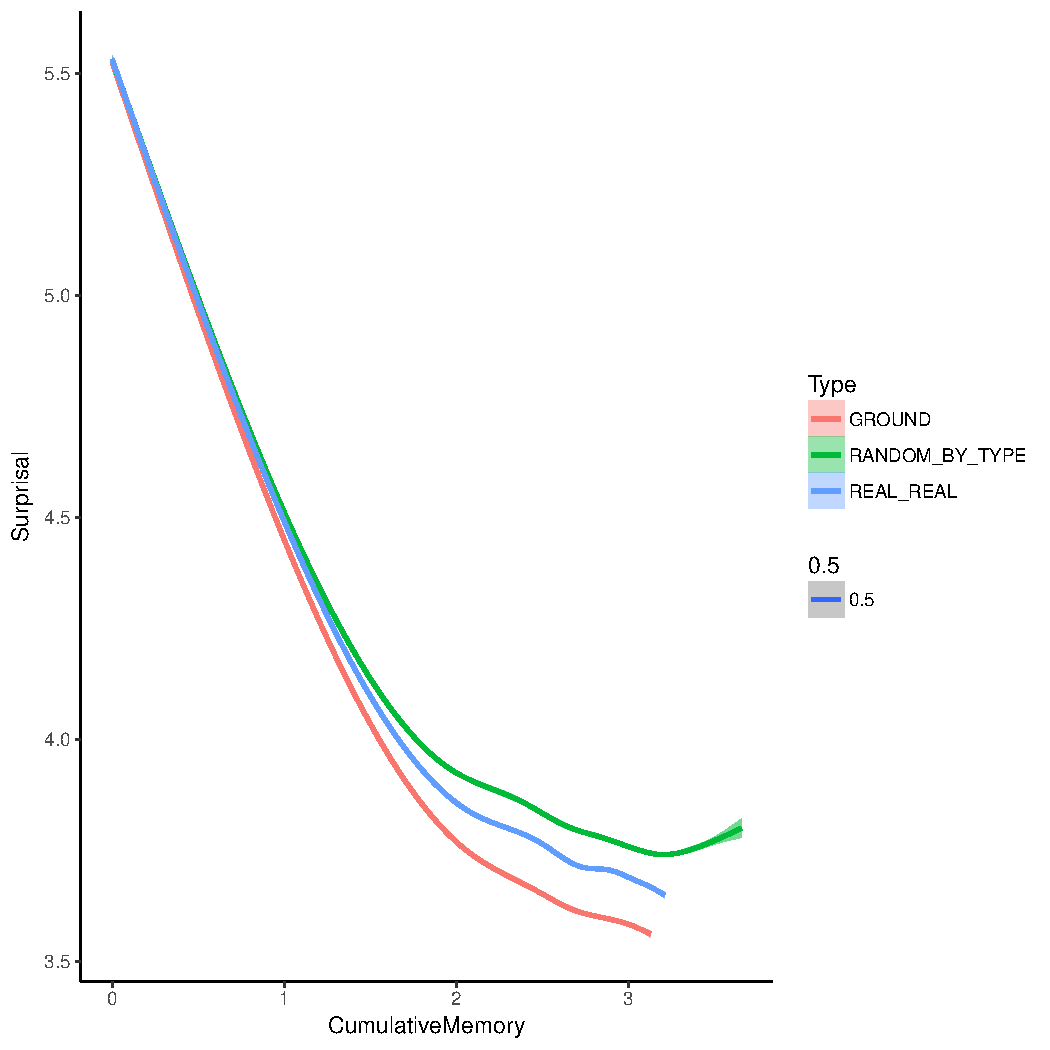
\includegraphics[width=0.25\textwidth]{figures/Czech-listener-surprisal-memory.pdf}}  &  $D_x$  \\ 
  &    &    &  $W_x$  &  1.0  &  [1.0, 1.0]  \\ [10.25ex] \hline
Danish  &  \multirow{4}{*}{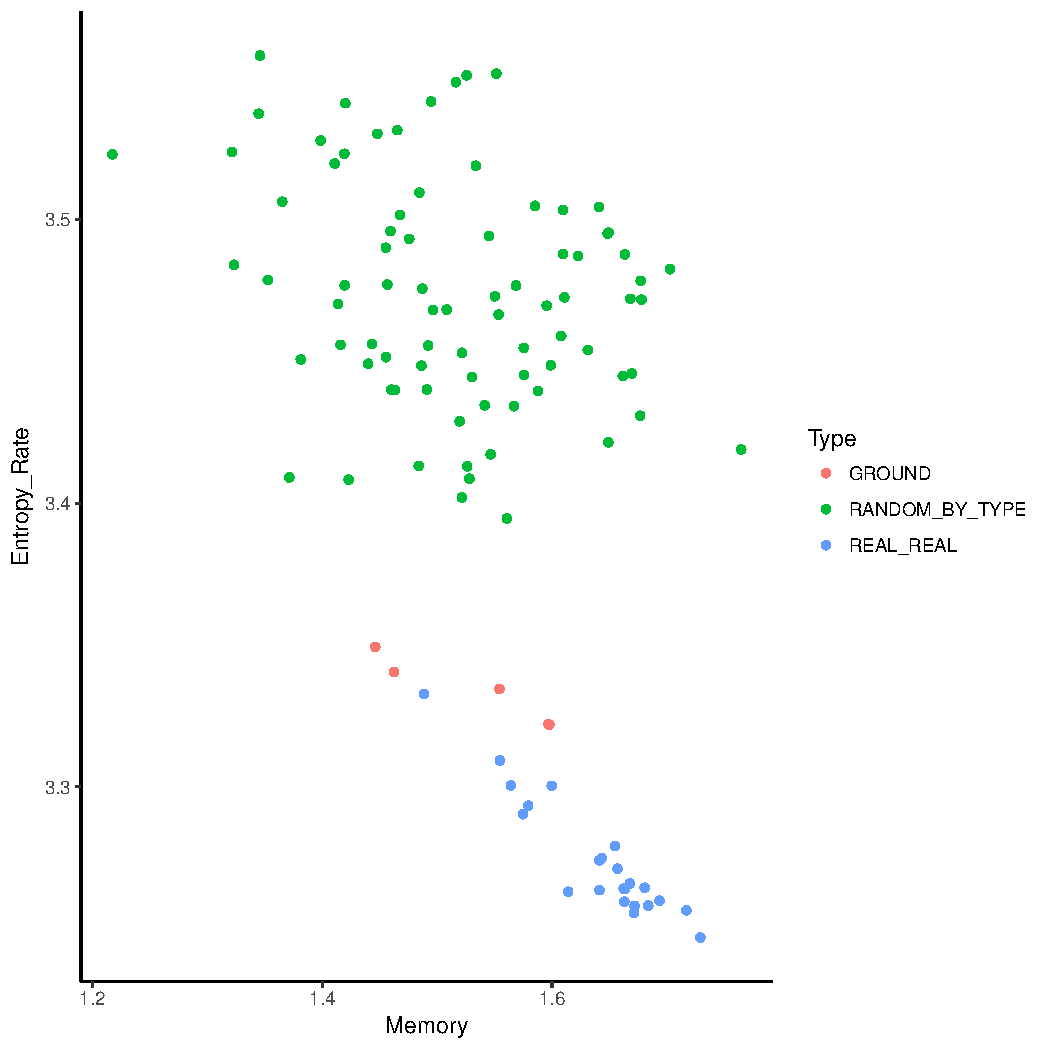
\includegraphics[width=0.25\textwidth]{figures/Danish-entropy-memory.pdf}}  &  \multirow{4}{*}{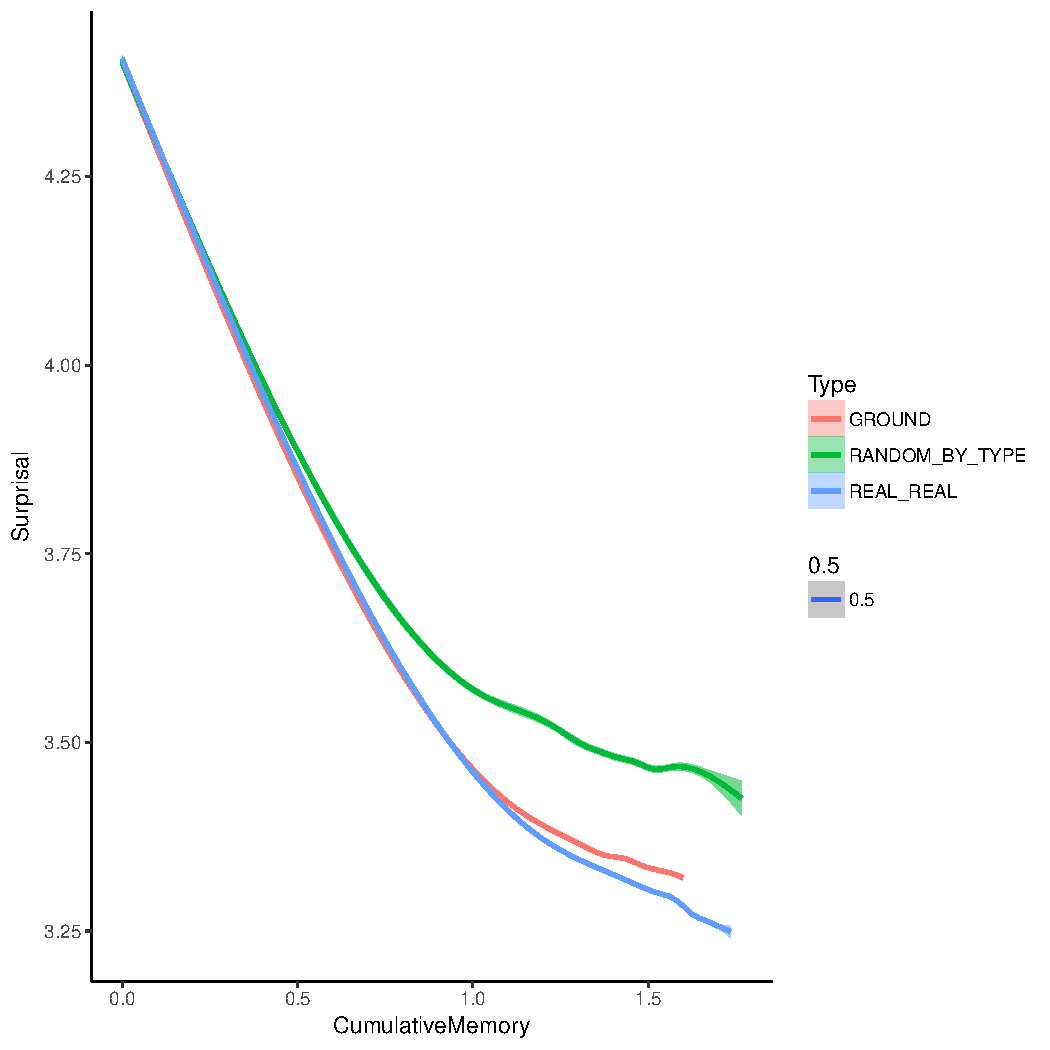
\includegraphics[width=0.25\textwidth]{figures/Danish-listener-surprisal-memory.pdf}}  &  $D_x$  \\ 
  &    &    &  $W_x$  &  1.0  &  [1.0, 1.0]  \\ [10.25ex] \hline
Dutch  &  \multirow{4}{*}{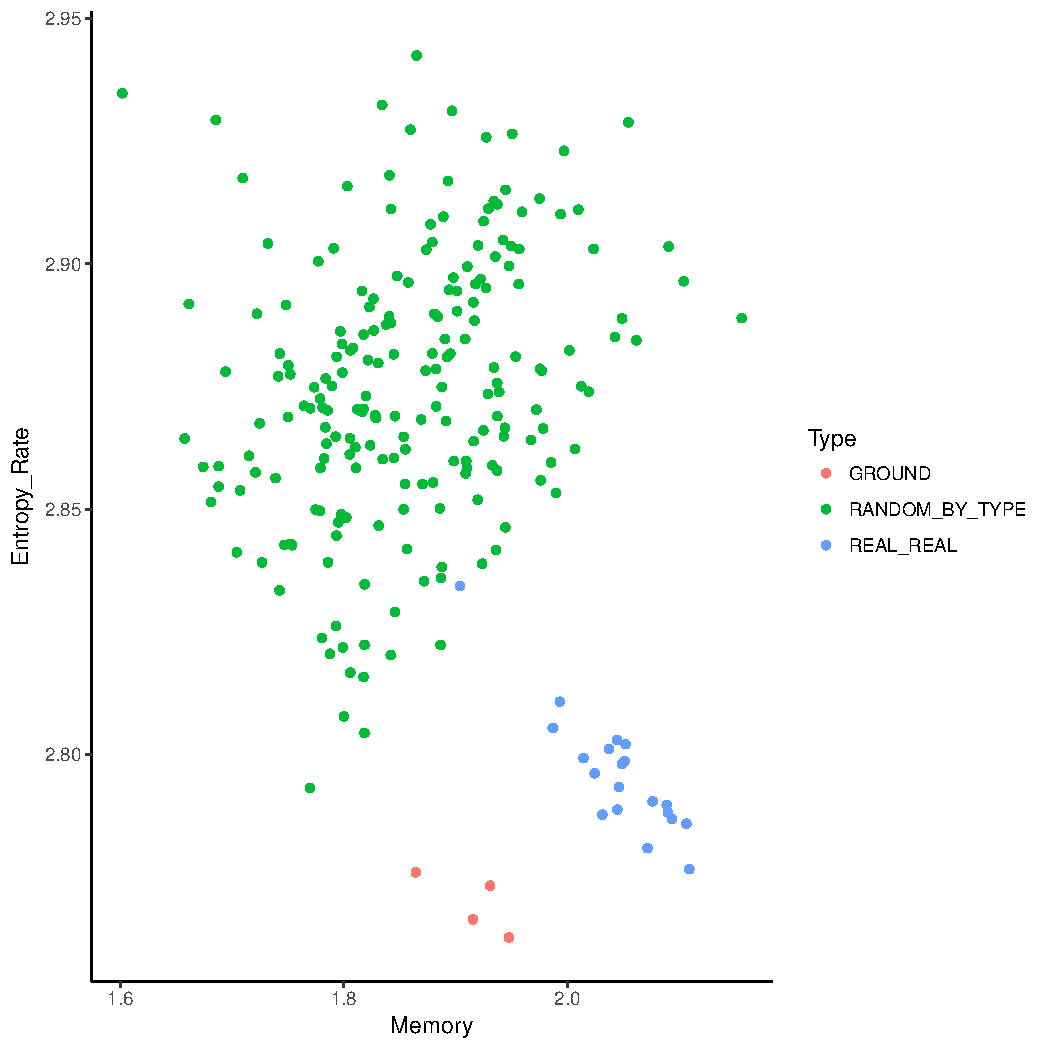
\includegraphics[width=0.25\textwidth]{figures/Dutch-entropy-memory.pdf}}  &  \multirow{4}{*}{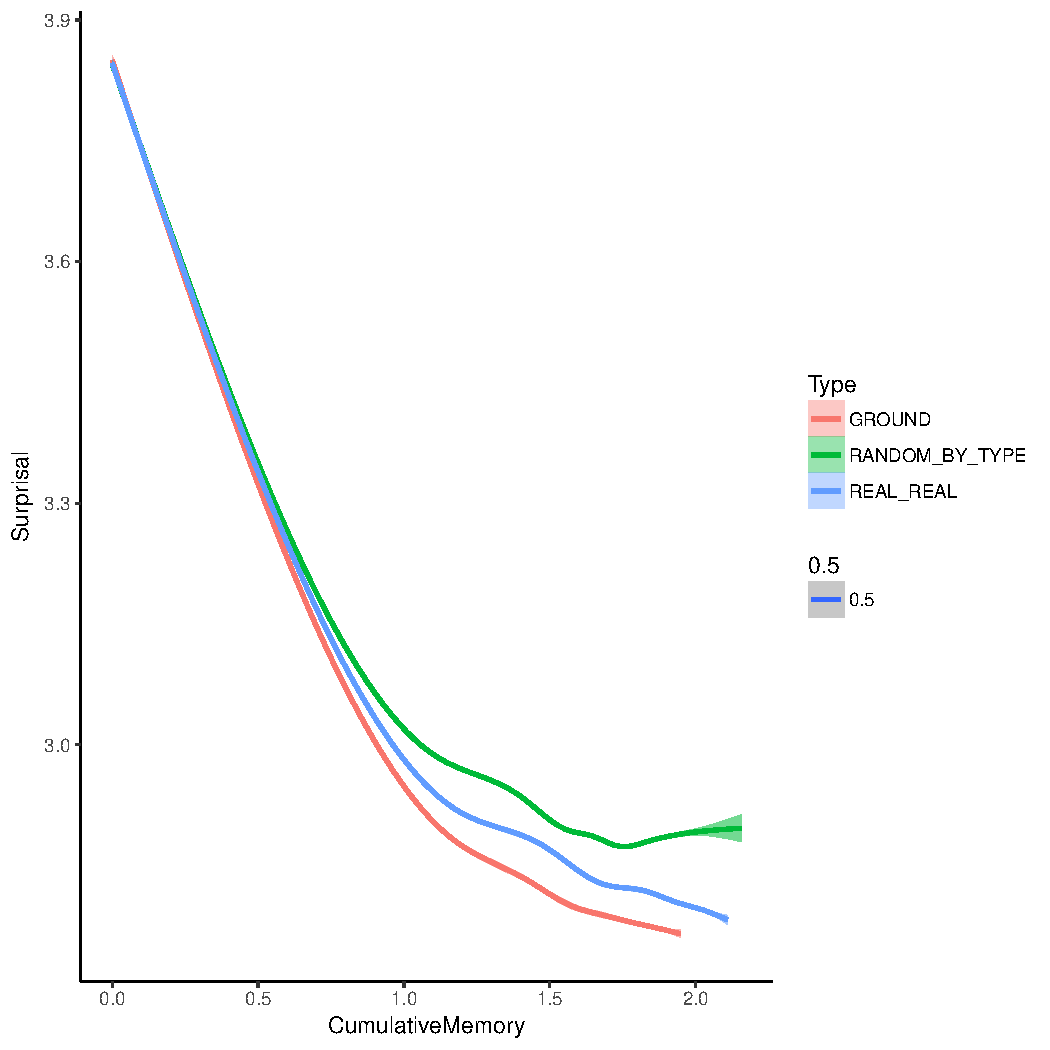
\includegraphics[width=0.25\textwidth]{figures/Dutch-listener-surprisal-memory.pdf}}  &  $D_x$  \\ 
  &    &    &  $W_x$  &  1.0  &  [1.0, 1.0]  \\ [10.25ex] \hline
English  &  \multirow{4}{*}{\includegraphics[width=0.25\textwidth]{figures/English-entropy-memory.pdf}}  &  \multirow{4}{*}{\includegraphics[width=0.25\textwidth]{figures/English-listener-surprisal-memory.pdf}}  &  $D_x$  \\ 
  &    &    &  $W_x$  &  1.0  &  [1.0, 1.0]  \\ [10.25ex] \hline
Erzya-Adap  &  \multirow{4}{*}{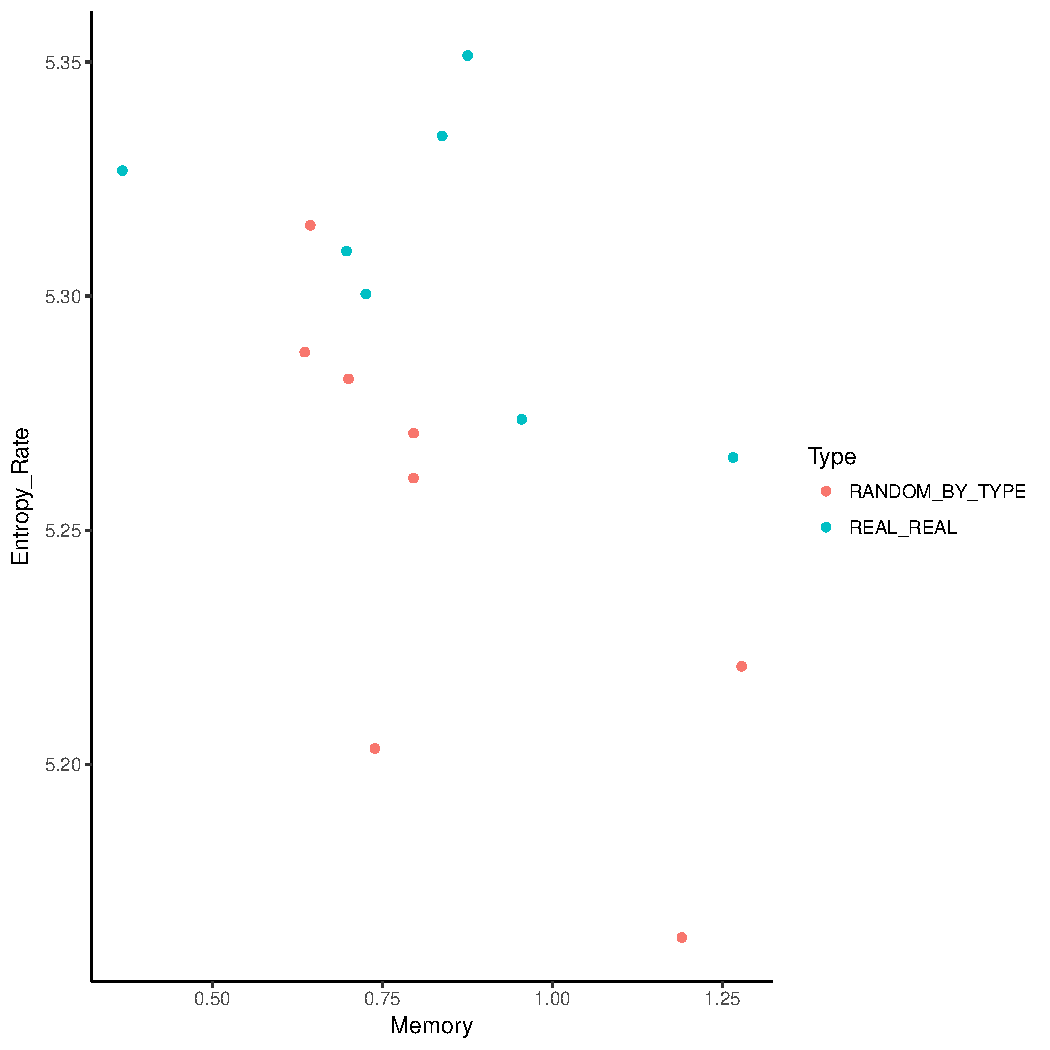
\includegraphics[width=0.25\textwidth]{figures/Erzya-Adap-entropy-memory.pdf}}  &  \multirow{4}{*}{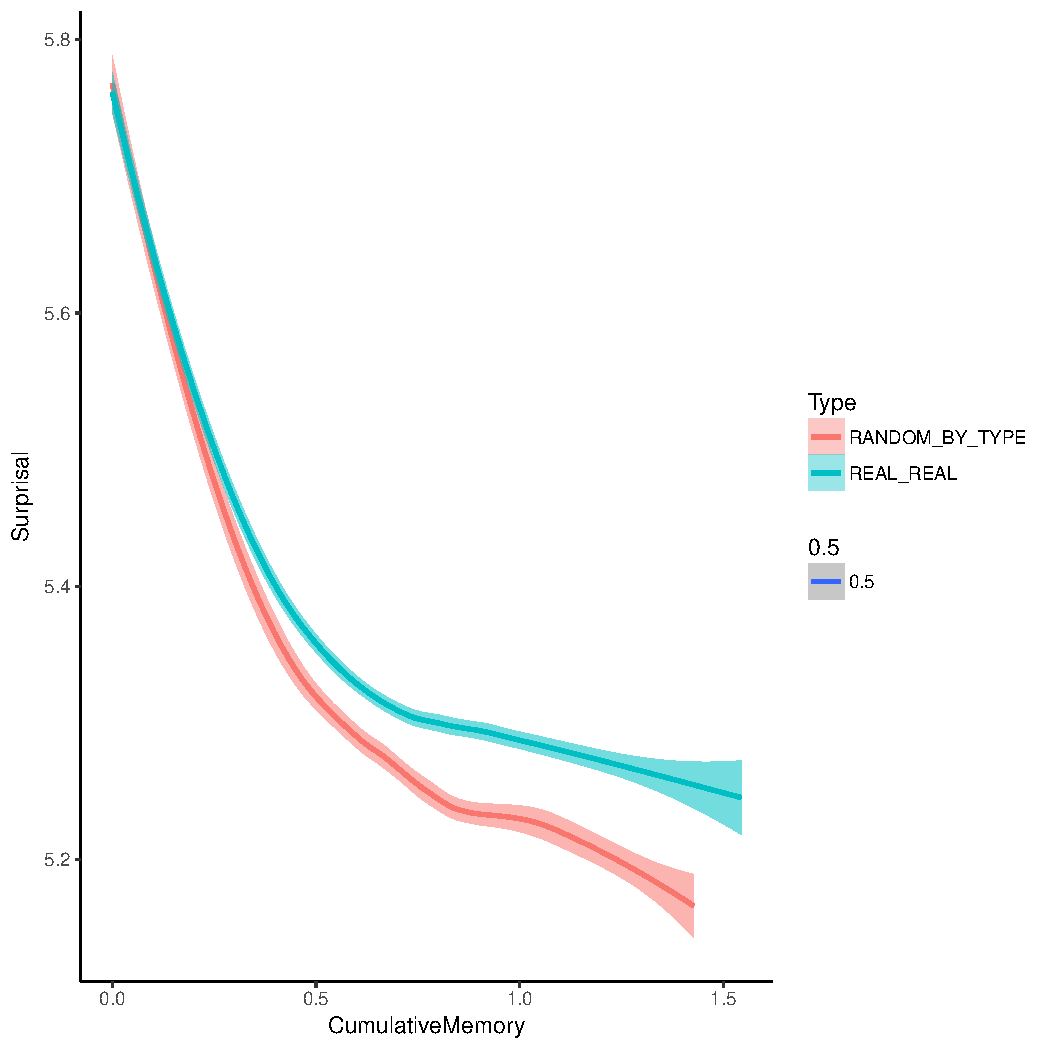
\includegraphics[width=0.25\textwidth]{figures/Erzya-Adap-listener-surprisal-memory.pdf}}  &  $D_x$  \\ 
  &    &    &  $W_x$  &  0.99  &  [0.98, 1.0]  \\ [10.25ex] \hline
Estonian  &  \multirow{4}{*}{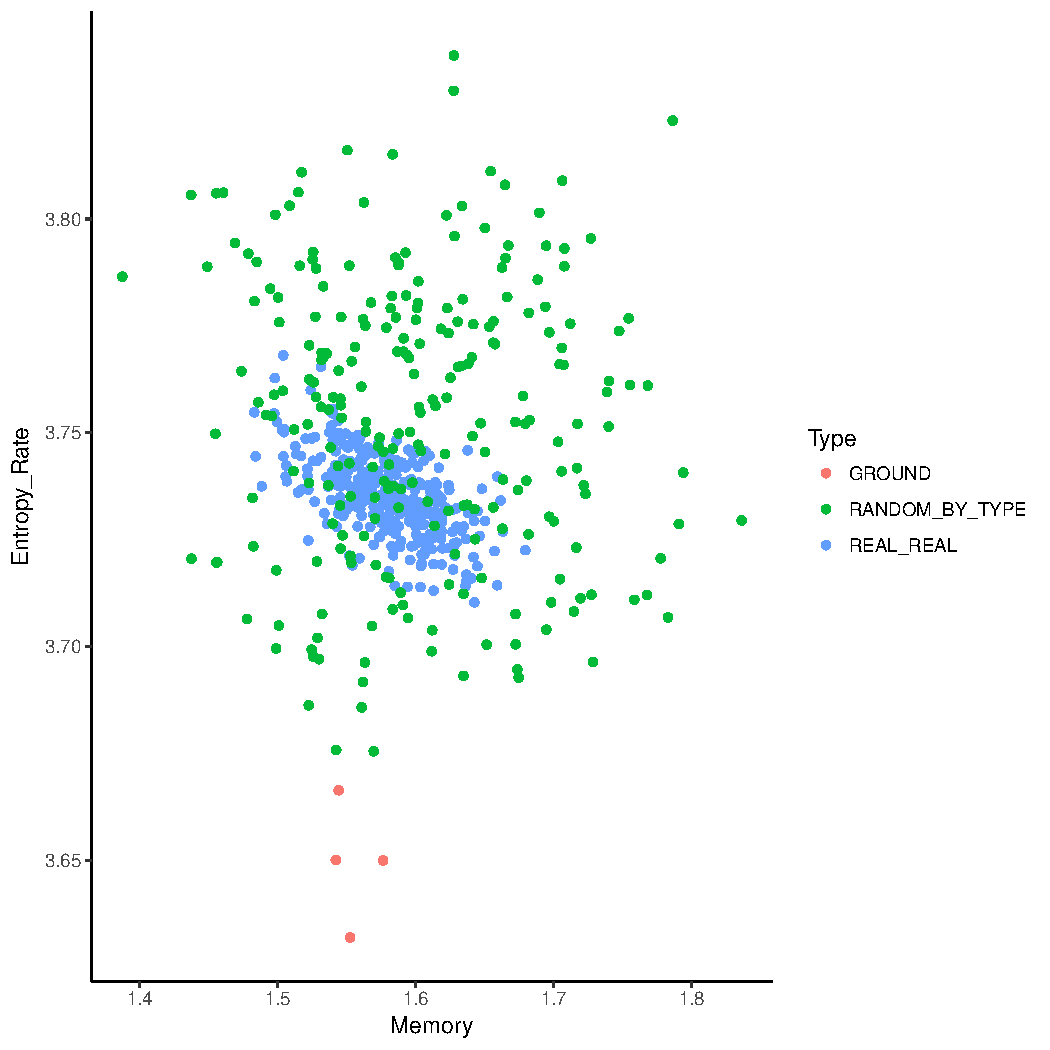
\includegraphics[width=0.25\textwidth]{figures/Estonian-entropy-memory.pdf}}  &  \multirow{4}{*}{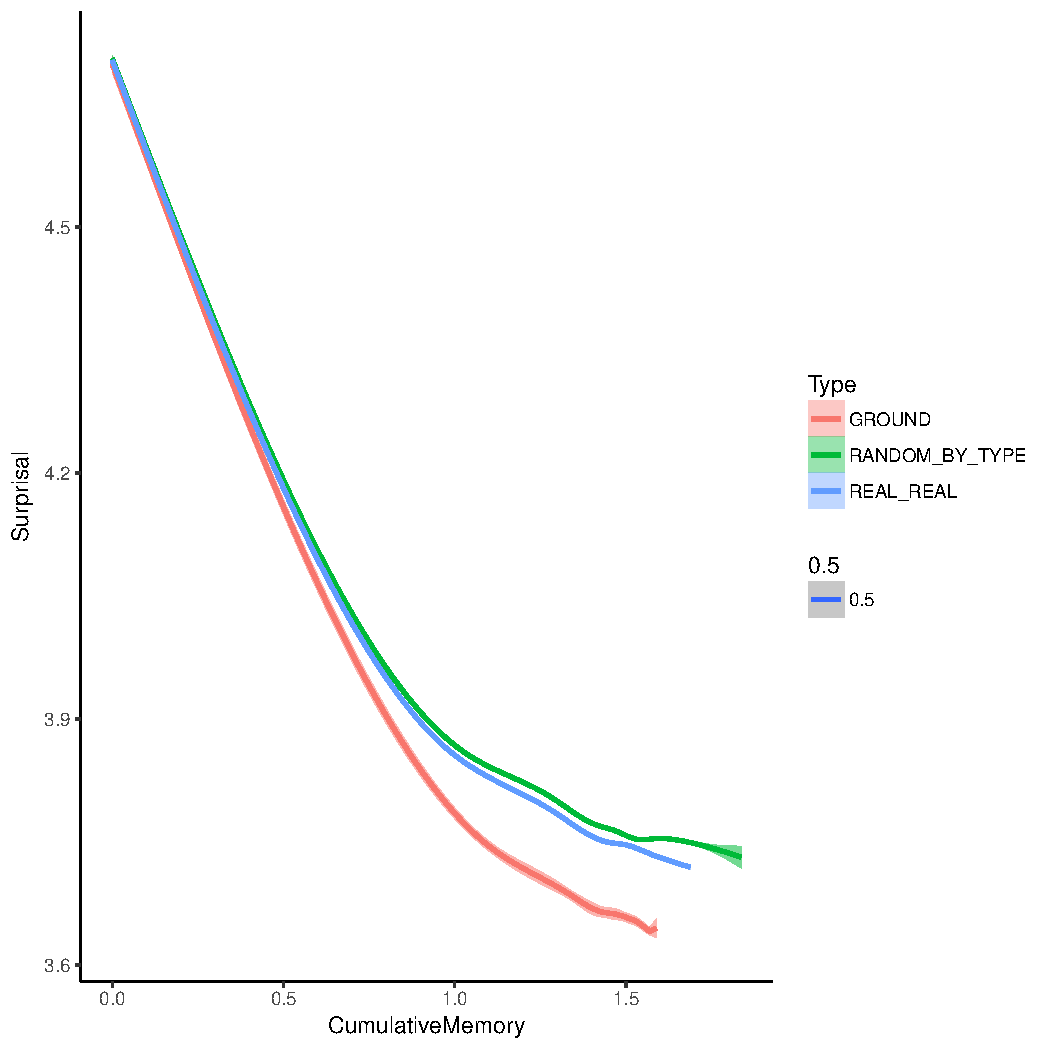
\includegraphics[width=0.25\textwidth]{figures/Estonian-listener-surprisal-memory.pdf}}  &  $D_x$  \\ 
  &    &    &  $W_x$  &  0.83  &  [0.76, 0.9]  \\ [10.25ex] \hline
Faroese-Adap  &  \multirow{4}{*}{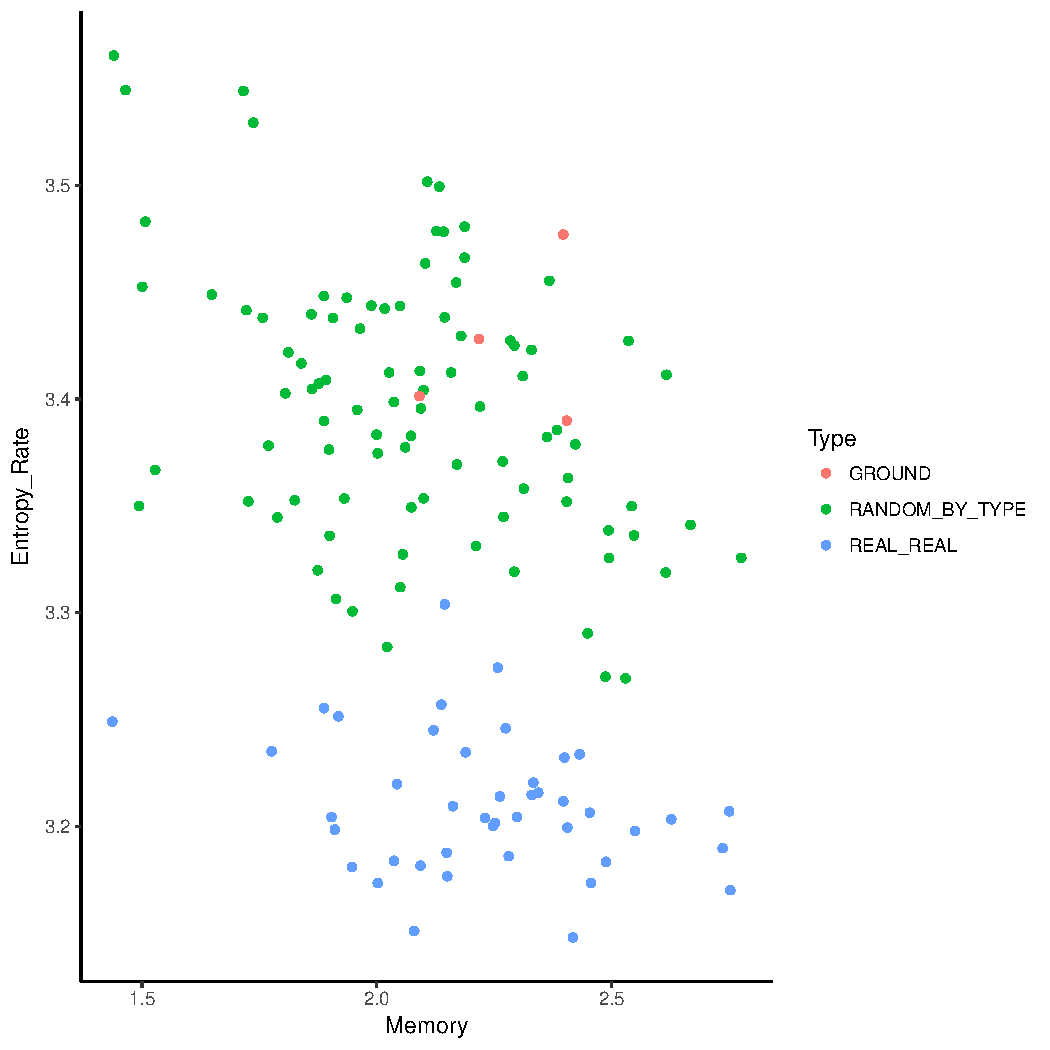
\includegraphics[width=0.25\textwidth]{figures/Faroese-Adap-entropy-memory.pdf}}  &  \multirow{4}{*}{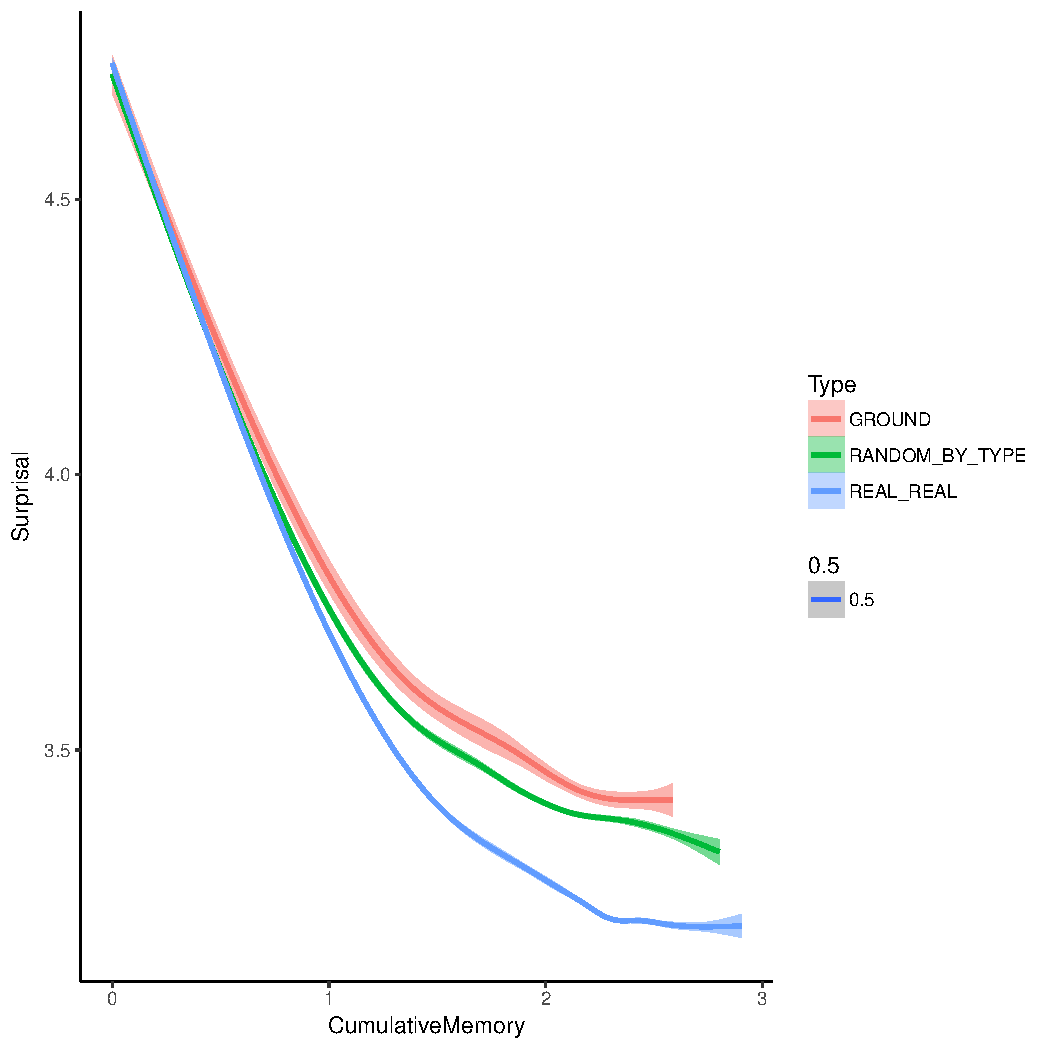
\includegraphics[width=0.25\textwidth]{figures/Faroese-Adap-listener-surprisal-memory.pdf}}  &  $D_x$  \\ 
  &    &    &  $W_x$  &  1.0  &  [1.0, 1.0]  \\ [10.25ex] \hline
Finnish  &  \multirow{4}{*}{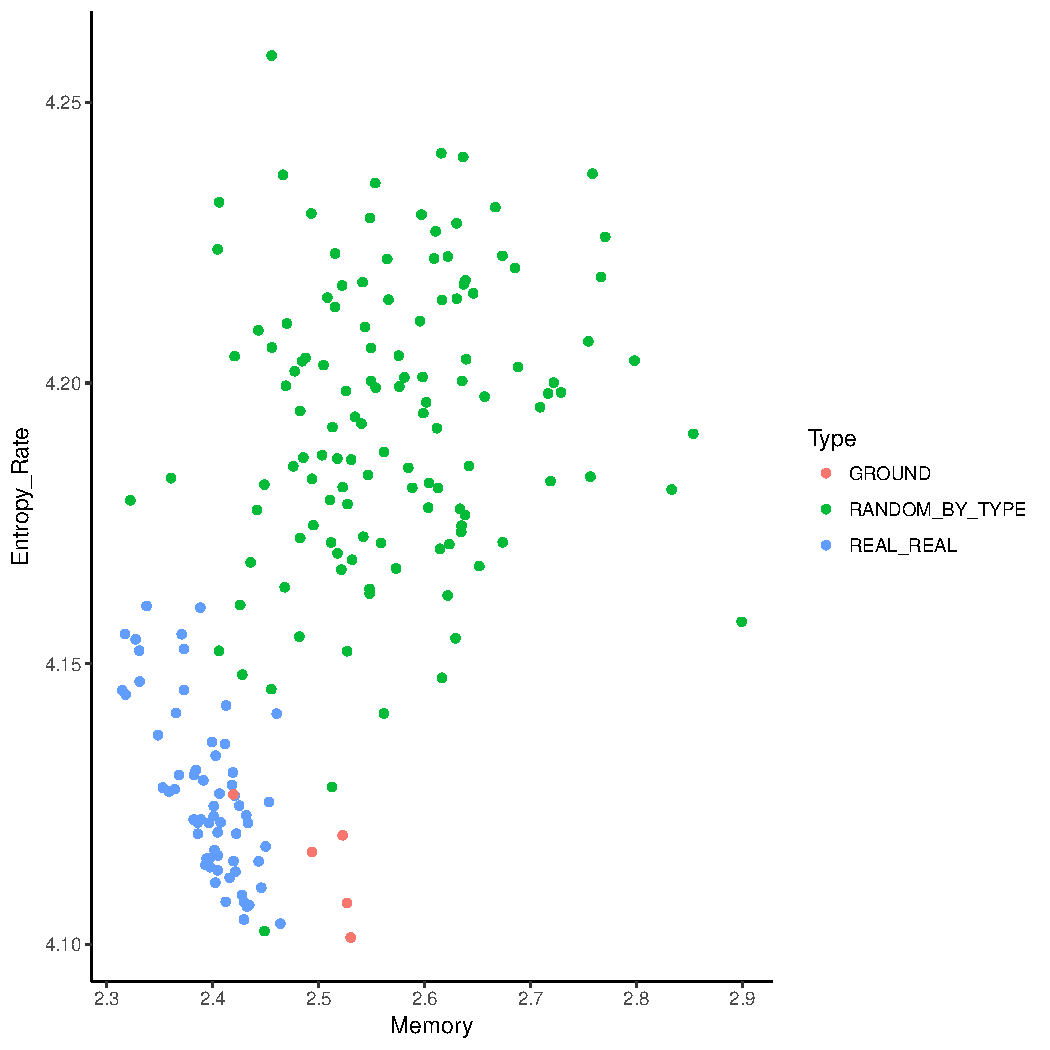
\includegraphics[width=0.25\textwidth]{figures/Finnish-entropy-memory.pdf}}  &  \multirow{4}{*}{\includegraphics[width=0.25\textwidth]{figures/Finnish-listener-surprisal-memory.pdf}}  &  $D_x$  \\ 
  &    &    &  $W_x$  &  1.0  &  [1.0, 1.0]  \\ [10.25ex] \hline
French  &  \multirow{4}{*}{\includegraphics[width=0.25\textwidth]{figures/French-entropy-memory.pdf}}  &  \multirow{4}{*}{\includegraphics[width=0.25\textwidth]{figures/French-listener-surprisal-memory.pdf}}  &  $D_x$  \\ 
  &    &    &  $W_x$  &  1.0  &  [1.0, 1.0]  \\ [10.25ex] \hline
German  &  \multirow{4}{*}{\includegraphics[width=0.25\textwidth]{figures/German-entropy-memory.pdf}}  &  \multirow{4}{*}{\includegraphics[width=0.25\textwidth]{figures/German-listener-surprisal-memory.pdf}}  &  $D_x$  \\ 
  &    &    &  $W_x$  &  1.0  &  [1.0, 1.0]  \\ [10.25ex] \hline
Greek  &  \multirow{4}{*}{\includegraphics[width=0.25\textwidth]{figures/Greek-entropy-memory.pdf}}  &  \multirow{4}{*}{\includegraphics[width=0.25\textwidth]{figures/Greek-listener-surprisal-memory.pdf}}  &  $D_x$  \\ 
  &    &    &  $W_x$  &  1.0  &  [1.0, 1.0]  \\ [10.25ex] \hline
Hebrew  &  \multirow{4}{*}{\includegraphics[width=0.25\textwidth]{figures/Hebrew-entropy-memory.pdf}}  &  \multirow{4}{*}{\includegraphics[width=0.25\textwidth]{figures/Hebrew-listener-surprisal-memory.pdf}}  &  $D_x$  \\ 
  &    &    &  $W_x$  &  1.0  &  [1.0, 1.0]  \\ [10.25ex] \hline
Hindi  &  \multirow{4}{*}{\includegraphics[width=0.25\textwidth]{figures/Hindi-entropy-memory.pdf}}  &  \multirow{4}{*}{\includegraphics[width=0.25\textwidth]{figures/Hindi-listener-surprisal-memory.pdf}}  &  $D_x$  \\ 
  &    &    &  $W_x$  &  1.0  &  [1.0, 1.0]  \\ [10.25ex] \hline
Hungarian  &  \multirow{4}{*}{\includegraphics[width=0.25\textwidth]{figures/Hungarian-entropy-memory.pdf}}  &  \multirow{4}{*}{\includegraphics[width=0.25\textwidth]{figures/Hungarian-listener-surprisal-memory.pdf}}  &  $D_x$  \\ 
  &    &    &  $W_x$  &  0.89  &  [0.81, 0.96]  \\ [10.25ex] \hline
Indonesian  &  \multirow{4}{*}{\includegraphics[width=0.25\textwidth]{figures/Indonesian-entropy-memory.pdf}}  &  \multirow{4}{*}{\includegraphics[width=0.25\textwidth]{figures/Indonesian-listener-surprisal-memory.pdf}}  &  $D_x$  \\ 
  &    &    &  $W_x$  &  1.0  &  [1.0, 1.0]  \\ [10.25ex] \hline
Japanese  &  \multirow{4}{*}{\includegraphics[width=0.25\textwidth]{figures/Japanese-entropy-memory.pdf}}  &  \multirow{4}{*}{\includegraphics[width=0.25\textwidth]{figures/Japanese-listener-surprisal-memory.pdf}}  &  $D_x$  \\ 
  &    &    &  $W_x$  &  1.0  &  [1.0, 1.0]  \\ [10.25ex] \hline
Kazakh-Adap  &  \multirow{4}{*}{\includegraphics[width=0.25\textwidth]{figures/Kazakh-Adap-entropy-memory.pdf}}  &  \multirow{4}{*}{\includegraphics[width=0.25\textwidth]{figures/Kazakh-Adap-listener-surprisal-memory.pdf}}  &  $D_x$  \\ 
  &    &    &  $W_x$  &  1.0  &  [1.0, 1.0]  \\ [10.25ex] \hline
Kurmanji-Adap*  &  \multirow{4}{*}{\includegraphics[width=0.25\textwidth]{figures/Kurmanji-Adap-entropy-memory.pdf}}  &  \multirow{4}{*}{\includegraphics[width=0.25\textwidth]{figures/Kurmanji-Adap-listener-surprisal-memory.pdf}}  &  $D_x$  \\ 
  &    &    &  $W_x$  &  0.92  &  [0.83, 0.99]  \\ [10.25ex] \hline
Latvian*  &  \multirow{4}{*}{\includegraphics[width=0.25\textwidth]{figures/Latvian-entropy-memory.pdf}}  &  \multirow{4}{*}{\includegraphics[width=0.25\textwidth]{figures/Latvian-listener-surprisal-memory.pdf}}  &  $D_x$  \\ 
  &    &    &  $W_x$  &  0.48  &  [0.4, 0.57]  \\ [10.25ex] \hline
Maltese  &  \multirow{4}{*}{\includegraphics[width=0.25\textwidth]{figures/Maltese-entropy-memory.pdf}}  &  \multirow{4}{*}{\includegraphics[width=0.25\textwidth]{figures/Maltese-listener-surprisal-memory.pdf}}  &  $D_x$  \\ 
  &    &    &  $W_x$  &  1.0  &  [1.0, 1.0]  \\ [10.25ex] \hline
Naija-Adap  &  \multirow{4}{*}{\includegraphics[width=0.25\textwidth]{figures/Naija-Adap-entropy-memory.pdf}}  &  \multirow{4}{*}{\includegraphics[width=0.25\textwidth]{figures/Naija-Adap-listener-surprisal-memory.pdf}}  &  $D_x$  \\ 
  &    &    &  $W_x$  &  1.0  &  [1.0, 1.0]  \\ [10.25ex] \hline
North Sami  &  \multirow{4}{*}{\includegraphics[width=0.25\textwidth]{figures/North_Sami-entropy-memory.pdf}}  &  \multirow{4}{*}{\includegraphics[width=0.25\textwidth]{figures/North_Sami-listener-surprisal-memory.pdf}}  &  $D_x$  \\ 
  &    &    &  $W_x$  &  0.37  &  [0.3, 0.44]  \\ [10.25ex] \hline
Norwegian  &  \multirow{4}{*}{\includegraphics[width=0.25\textwidth]{figures/Norwegian-entropy-memory.pdf}}  &  \multirow{4}{*}{\includegraphics[width=0.25\textwidth]{figures/Norwegian-listener-surprisal-memory.pdf}}  &  $D_x$  \\ 
  &    &    &  $W_x$  &  1.0  &  [1.0, 1.0]  \\ [10.25ex] \hline
Persian  &  \multirow{4}{*}{\includegraphics[width=0.25\textwidth]{figures/Persian-entropy-memory.pdf}}  &  \multirow{4}{*}{\includegraphics[width=0.25\textwidth]{figures/Persian-listener-surprisal-memory.pdf}}  &  $D_x$  \\ 
  &    &    &  $W_x$  &  1.0  &  [1.0, 1.0]  \\ [10.25ex] \hline
Polish  &  \multirow{4}{*}{\includegraphics[width=0.25\textwidth]{figures/Polish-entropy-memory.pdf}}  &  \multirow{4}{*}{\includegraphics[width=0.25\textwidth]{figures/Polish-listener-surprisal-memory.pdf}}  &  $D_x$  \\ 
  &    &    &  $W_x$  &  0.07  &  [0.01, 0.15]  \\ [10.25ex] \hline
Portuguese  &  \multirow{4}{*}{\includegraphics[width=0.25\textwidth]{figures/Portuguese-entropy-memory.pdf}}  &  \multirow{4}{*}{\includegraphics[width=0.25\textwidth]{figures/Portuguese-listener-surprisal-memory.pdf}}  &  $D_x$  \\ 
  &    &    &  $W_x$  &  1.0  &  [1.0, 1.0]  \\ [10.25ex] \hline
Romanian  &  \multirow{4}{*}{\includegraphics[width=0.25\textwidth]{figures/Romanian-entropy-memory.pdf}}  &  \multirow{4}{*}{\includegraphics[width=0.25\textwidth]{figures/Romanian-listener-surprisal-memory.pdf}}  &  $D_x$  \\ 
  &    &    &  $W_x$  &  1.0  &  [1.0, 1.0]  \\ [10.25ex] \hline
Serbian  &  \multirow{4}{*}{\includegraphics[width=0.25\textwidth]{figures/Serbian-entropy-memory.pdf}}  &  \multirow{4}{*}{\includegraphics[width=0.25\textwidth]{figures/Serbian-listener-surprisal-memory.pdf}}  &  $D_x$  \\ 
  &    &    &  $W_x$  &  1.0  &  [1.0, 1.0]  \\ [10.25ex] \hline
Slovak  &  \multirow{4}{*}{\includegraphics[width=0.25\textwidth]{figures/Slovak-entropy-memory.pdf}}  &  \multirow{4}{*}{\includegraphics[width=0.25\textwidth]{figures/Slovak-listener-surprisal-memory.pdf}}  &  $D_x$  \\ 
  &    &    &  $W_x$  &  0.07  &  [0.03, 0.12]  \\ [10.25ex] \hline
Slovenian  &  \multirow{4}{*}{\includegraphics[width=0.25\textwidth]{figures/Slovenian-entropy-memory.pdf}}  &  \multirow{4}{*}{\includegraphics[width=0.25\textwidth]{figures/Slovenian-listener-surprisal-memory.pdf}}  &  $D_x$  \\ 
  &    &    &  $W_x$  &  0.82  &  [0.74, 0.89]  \\ [10.25ex] \hline
Spanish  &  \multirow{4}{*}{\includegraphics[width=0.25\textwidth]{figures/Spanish-entropy-memory.pdf}}  &  \multirow{4}{*}{\includegraphics[width=0.25\textwidth]{figures/Spanish-listener-surprisal-memory.pdf}}  &  $D_x$  \\ 
  &    &    &  $W_x$  &  1.0  &  [1.0, 1.0]  \\ [10.25ex] \hline
Swedish  &  \multirow{4}{*}{\includegraphics[width=0.25\textwidth]{figures/Swedish-entropy-memory.pdf}}  &  \multirow{4}{*}{\includegraphics[width=0.25\textwidth]{figures/Swedish-listener-surprisal-memory.pdf}}  &  $D_x$  \\ 
  &    &    &  $W_x$  &  1.0  &  [1.0, 1.0]  \\ [10.25ex] \hline
Thai-Adap  &  \multirow{4}{*}{\includegraphics[width=0.25\textwidth]{figures/Thai-Adap-entropy-memory.pdf}}  &  \multirow{4}{*}{\includegraphics[width=0.25\textwidth]{figures/Thai-Adap-listener-surprisal-memory.pdf}}  &  $D_x$  \\ 
  &    &    &  $W_x$  &  1.0  &  [1.0, 1.0]  \\ [10.25ex] \hline
Turkish  &  \multirow{4}{*}{\includegraphics[width=0.25\textwidth]{figures/Turkish-entropy-memory.pdf}}  &  \multirow{4}{*}{\includegraphics[width=0.25\textwidth]{figures/Turkish-listener-surprisal-memory.pdf}}  &  $D_x$  \\ 
  &    &    &  $W_x$  &  1.0  &  [1.0, 1.0]  \\ [10.25ex] \hline
Ukrainian  &  \multirow{4}{*}{\includegraphics[width=0.25\textwidth]{figures/Ukrainian-entropy-memory.pdf}}  &  \multirow{4}{*}{\includegraphics[width=0.25\textwidth]{figures/Ukrainian-listener-surprisal-memory.pdf}}  &  $D_x$  \\ 
  &    &    &  $W_x$  &  1.0  &  [1.0, 1.0]  \\ [10.25ex] \hline
Urdu  &  \multirow{4}{*}{\includegraphics[width=0.25\textwidth]{figures/Urdu-entropy-memory.pdf}}  &  \multirow{4}{*}{\includegraphics[width=0.25\textwidth]{figures/Urdu-listener-surprisal-memory.pdf}}  &  $D_x$  \\ 
  &    &    &  $W_x$  &  1.0  &  [1.0, 1.0]  \\ [10.25ex] \hline
Uyghur-Adap*  &  \multirow{4}{*}{\includegraphics[width=0.25\textwidth]{figures/Uyghur-Adap-entropy-memory.pdf}}  &  \multirow{4}{*}{\includegraphics[width=0.25\textwidth]{figures/Uyghur-Adap-listener-surprisal-memory.pdf}}  &  $D_x$  \\ 
  &    &    &  $W_x$  &  0.65  &  [0.57, 0.74]  \\ [10.25ex] \hline
Vietnamese  &  \multirow{4}{*}{\includegraphics[width=0.25\textwidth]{figures/Vietnamese-entropy-memory.pdf}}  &  \multirow{4}{*}{\includegraphics[width=0.25\textwidth]{figures/Vietnamese-listener-surprisal-memory.pdf}}  &  $D_x$  \\ 
  &    &    &  $W_x$  &  1.0  &  [0.98, 1.0]  \\ [10.25ex] \hline

\end{longtable}




\begin{figure}
\includegraphics[width=0.95\textwidth]{neural/figures/full-REAL-listener-surprisal-memory-HIST_z_byMem_onlyWordForms_boundedVocab.pdf}
	\caption{Histogram}\label{fig:hist-real}
\end{figure}

\subsection{Discussion}

All four languages have relatively strong word order freedom.
We hypothesized that freedom of word order freedm may be responsible for the difference between these languages and the other languages.
We quantified word order freedom as the branching direction entropy~\cite{futrell-quantifying-2015}.
We found that branching direction entropy was strongly correlated with the surprisal difference between real and baseline orderings (Spearman correlations -0.58, $p = 7.414e-6$).



\begin{figure}
\includegraphics[width=0.95\textwidth]{neural/figures/surprisal-branching-entropy-REAL.pdf}
	\caption{Surprisal Difference vs Branching Direction Entropy.}\label{fig:hist-real}
\end{figure}






\section{Fixed Word Orders}

We test this hypothesis by comparing baseline languages to \emph{fixed-order} versions of the real languages.
This enables us to tease apart the impact of the languages' word order rules from the impact of more specific ordering choices.


\begin{figure}
\includegraphics[width=0.95\textwidth]{neural/figures/full-GROUND-listener-surprisal-memory-HIST_z_byMem_onlyWordForms_boundedVocab.pdf}
	\caption{Histogram}\label{fig:hist-real}
\end{figure}




\bibliographystyle{apalike}
\bibliography{literature}

\appendix

\section{Experiment with MLE Grammars}


\paragraph{Maximum-Likelihood Grammars}
We additionally create ordering grammars that are fit to the actual orderings of each language.
These grammars faithfully represent the ordering rules if the actual language, to the extent that is possible in the formalism of ordering grammars.

We construct these grammars by interpreting ordering grammars probabilistically, and setting the parameters 


We found that, across treebanks, random grammars that have more fine-grained rules or are evaluated nondeterministically do worse in both memory-surprisal tradeoffs.
Thus, random grammars with by-relation weights constitute a stronger baseline.



\section{N-Gram Models}



\section{Morphology-Based Encoding}



Held-out:

- UD languages:

-- English, Korean, Russian

-- UD$\_$Polish-LFG (released in 2.2, not included in original experiment) (13,744 sentences)

-- character-level Russian




\section{Character-Level Modeling}

\section{Non-UD Dependency Treebanks}



- other treebanks



-- spoken Japanese (T{\"u}ba-J/S)

-- another Vietnamese dependency treebank \citep{nguyen-bktreebank:-2017} (5,639 sentences)


-- another Chinese dependency treebank LDC2012T05


Due to the sizes of these treebanks, can also do experiment with full word forms.


\section{Constituency Treebank}

-- Penn treebank \citep{marcus-building-1993}

-- spoken English (T{\"u}ba-E/S)

-- spoken German (T{\"u}ba-D/S)

-- Chinese treebank \citep{xue-chinese-2013}


\section{Proofs}



\begin{proof}
We denote the listener's memory state after hearing $X_{<t}$ by $L_t$.
The average number of bits required to encode this state is $H[L_t]$, which by assumption is at most $\sum_{t=1}^T t I_t$.
As the listener's predictions are made on the basis of her memory state, her average surprisal is at least $H[X_t | L_t]$.
The difference between the listener's surprisal and optimal surprisal is thus at least $H[X_t | L_t] - H[X_t | X_{<t}]$.
By stationarity, we can rewrite this expression as
\begin{align*}
	H[X_t | L_t] - H[X_t | X_{<t}] &=  \frac{1}{T} \sum_{t=1}^{T} \left(H[X_t | L_t] - H[X_t | X_{<t}]\right) 
\end{align*}
For any $t$,
	\begin{equation}
H[X_t | L_t] \geq H[X_t| X_{t-1}, L_{t-1}] \geq ... \geq H[X_t|X_{1 \dots t-1}, L_0]
		\end{equation}
	This can be derived from the two conditions \ref{eq:listener-markov-1} and \ref{eq:listener-markov-2} (TODO explain how).

	\begin{equation}
H[X_t| X_{2 \dots t-1}, L_{1}] \geq H[X_t|X_{1 \dots t-1}, L_0]
	\end{equation}
is true because the following is a Markov chain:
\begin{equation}
(X_t) \rightarrow (L_0, X_1, X_{2 \dots t-1})   \rightarrow   (L_1, X_{2 \dots t-1})
\end{equation}
because
\begin{align*}
p(X_t|L_0, X_1, X_{2 \dots t-1}; L_1, X_{2 \dots t-1}) & = p(X_t|L_0, L_1, X_1, X_{2 \dots t-1}) \\
& = \sum_{X_{<1}} p(X_t|X_{<1}, L_0, L_1, X_1, X_{2 \dots t-1}) p(X_{<1}| L_0, L_1, X_1, X_{2 \dots t-1}) \\
&= \sum_{X_{<1}} p(X_t|X_{<1}, L_0,  X_1, X_{2 \dots t-1}) p(X_{<1}| L_0, X_1, X_{2 \dots t-1}) \\
&= p(X_t|L_0,  X_1, X_{2 \dots t-1}) 
\end{align*}
because
	\begin{align*}
p(X_t|X_{<1}, L_0, L_1, X_1, X_{2 \dots t-1}) = p(X_t|X_{<1}, L_0,  X_1, X_{2 \dots t-1}) \\
p(X_{<1}| L_0, L_1, X_1, X_{2 \dots t-1})   = p(X_{<1}| L_0, X_1, X_{2 \dots t-1})
	\end{align*}
because of Equation~\ref{eq:listener-markov}.
	\begin{equation}
p((X_{t})_t| L_0, L_1, X_1)   = p((X_{t})_t| L_0, X_1)
	\end{equation}

	
	% = \int dX_{<1} p(X_t|X_{<1}, X_1, X_{2 \dots t-1})  = \int dX_{<1} p(X_t|L_0, X_{<1}, X_1, X_{2 \dots t-1}) = p(X_t|L_0, X_1, X_{2 \dots t-1}) $

%	$p(X_t|L_0, X_1, X_{2 \dots t-1}; L_1, X_{2 \dots t-1}) = p(X_t|L_0, L_1, X_1, X_{2 \dots t-1}) = \int dX_{<1} p(X_t|X_{<1}, L_0, L_1, X_1, X_{2 \dots t-1}) = \int dX_{<1} p(X_t|X_{<1}, X_1, X_{2 \dots t-1})  = \int dX_{<1} p(X_t|L_0, X_{<1}, X_1, X_{2 \dots t-1}) = p(X_t|L_0, X_1, X_{2 \dots t-1}) $

Therefore
\begin{align*}
	H[X_t | L_t] - H[X_t | X_{<t}]& \geq \frac{1}{T} \sum_{t=1}^T ( H[X_t|X_{1\dots t-1}, L_0] - H[X_t | X_{1\dots t-1}, X_{\leq 0}]  )    \\
	& = \frac{1}{T} \left(H[X_{1\dots T} | L_0] - H[X_{1\dots T} | X_{\leq 0}]\right)  \\
	& = \frac{1}{T} \left(I[X_{1\dots T}|X_{\leq 0}] - I[X_{1\dots T}|L_0]\right) 
\end{align*}
	The first term $I[X_{1\dots T}|X_{\leq 0}]$ can be rewritten in terms of $I_t$:
\begin{align*}
	H[X_t | L_t] - H[X_t | X_{<t}]& \geq \frac{1}{T} \left(\sum_{t=1}^T t I_t + T \sum_{t > T} I_t - I[X_{1\dots T}|L_0]\right) 
	%	&= \frac{1}{T} \left(\sum_{t=1}^\infty t I_t - \sum_{t > T}  (T-t) I_t- I[X_{1\dots T}|L_0]\right) \\
\end{align*}
	$I[X_{1\dots T}|L_0]$ is at most $H[L_0]$, which is at most $\sum_{t=1}^T t I_t$ by assumption. Thus, the expression above is bounded by
	\begin{align*}
	H[X_t | L_t] - H[X_t | X_{<t}]& \geq \frac{1}{T} \left(\sum_{t=1}^T t I_t + T \sum_{t > T} I_t - \sum_{t=1}^T t I_t\right) \\
		&= \sum_{t > T} I_t
\end{align*}
	Rearranging shows that the listener's surprisal is at least $H[X_t|L_t] \geq H[X_t | X_{<t}] + \sum_{t > T} I_t$, as claimed.
\end{proof}





\end{document}






